\documentclass[12px]{article}

\title{Dispense Algebra I\\[5px] \normalsize Prima parte del corso}
\date{2024-12-22}
\author{Federico De Sisti}

\input{../../setup.tex}

\begin{document}
	\maketitle
	\newpage

	\tableofcontents
	\newpage


	\section{Preambolo}
	Siamo giunti a un nuovo capitolo della nostra vita. A volte, per andare avanti, è necessario guardarsi un po' indietro; altre volte, per dimostrare un teorema, bisogna osare e andare oltre l'uso delle semplici ipotesi, arrivando persino a utilizzare la stessa tesi che vogliamo comprovare. L'algebra, in fondo, non è solo una raccolta di regole e teoremi, ma un modo per guardare il mondo con nuovi occhi e trovare connessioni inaspettate tra idee apparentemente lontane.\\[10px]
	Questa dispensa non è solo un supporto didattico, ma un piccolo viaggio da percorrere insieme, fatto di curiosità, sfide e, perché no, qualche sorriso lungo il cammino. Alberto, con il suo cuore così grande, riesce a infondere a tutti noi un po' della sua energia: la stessa che distribuisce periodicamente nell’aula 1, per evitare che esploda di entusiasmo.\\[10px]
	Un ringraziamento speciale va alla redazione, che con impegno e creatività ha reso tutto questo possibile: Marco (dai capelli lunghi, anche se, da quando hanno aperto un barbiere a Civita, un po' meno lunghi), Gabriel (sempre nel flusso, come un’equazione ben bilanciata), Fabio (compagno di merende a mensa, con cui ogni pausa si trasforma in un momento memorabile) e Simone (che, quando riesci a incontrarlo, sa sempre come strapparti un sorriso).\\[10px]
	E infine, un augurio a Simone affinché possa finalmente avere la meglio sul suo nemico più temuto: LPC. Perché, in fondo, ogni battaglia può essere vinta con la giusta determinazione e un pizzico di algebra.\\[10px]
Buona lettura e buon viaggio in questo affascinante mondo che, come una funzione complessa, nasconde sempre qualcosa di meraviglioso appena dietro l’angolo.\ \\ \vfill \ \\
	P.S. Se non avete stampato queste dispense tramite l'autore siete un mucchio di stronzi.\\
	P.P.S. Si ringrazia OpenAI per l'immensa saggezza nella formulazione di questo preambolo, con qualche dritta, sorprende sempre.
\newpage

	\section{Cosa c'è su e-leaning di Francesco Mazzini}
	Date appelli\\
	Esercizi settimanali\\
	All'esame ti chiedono due esercizi delle schede scelti a caso\\
	Ci sono 2 esoneri (primo 17 dicembre) (secondo ?? maggio)\\
\textbf{Libri}\\
M. Artin Algebra\\
IN. Hernstein: Algebra (difficile)\\
\section{Gruppi}
\begin{defi}[Gruppo]
	Un gruppo è un dato di un insieme $G$ con un'operazione $\cdot$ tali che:\\
	1) L'operazione è associativa\\
	\[f \cdot (g\codt h) = (f\cdot g)\cdot h \ \ \ \ \ \forall f, g, h\in G\]
	2) Esistenza elemento neutro
	\[
		\exists e\in G \text{    tale che     } g\cdot e = e\cdot g = g \ \ \ \forall g\in G
	.\] 
	3) esistenza degli inversi
	\[
		\forall g\in G \ \ \ \ \ \exists \ \ \ \ g^{-1}\in G \ \ \text{ tale che    } g^{-1}\cdot g = g\cdot g^{-1} = e
	.\] 
\end{defi}
\begin{nome}[notazione]
	$(G,\cdot)$
	dato  $g\in G$ denotiamo con: \\
	1) g^0 = e\\
	2) g^1 = g\\
	3) g^n = g\cdot\ldots\cdot g\\
	4) g^{-n} = (g^{-1})^n

\end{nome}
\textbf{Osservazione:}\\
Con questa notazione:\\
\[
	(g^n)^m = g^{nm}
\] 
\[
	g^n \cdot g^m = g^{n + m}
\] 
\textbf{Esempi}\\
1) $(\mathbb Z, + ), (\mathbb Q, + ), (\R, +)$\\
2)  $GL_n(\K) = \lbrace{A\in Mat_{n\times n}(\K) | det(A) \neq 0\rbrace$ con prodotto\\
	3) $SL_n(\K) = \lbraceA\in Mat_{nn}(\K) | det(A) = 1\rbrace$\\
4) $X$ insieme\\
\text{ } \hspace{90px} $S_X = \lbrace$ funzioni  $X \rightarrow X$ invertibili$\rbrace$\\
\textbf{Speciale}
Se $X = \lbrace 1,\ldots, n\rbrace}$\\
Allora chiamiamo 
 \[
S_n = S_X
.\] 
(è il gruppo di permutazioni su $n$ elementi)\\
Si chiama gruppo simmetrico
\begin{defi}[Gruppo diedrale]
	$n\geq 3$ Consideriamo l'n-agono regolare nel piano (3-agono, triangolo)\\
	 $D_n$ è l'insieme delle simmetrie del piano che preservano l' $n$-agono\\
	 Si chiama gruppo diedrale, l'operazione è la composizione
\end{defi}
\textbf{Esempio:}\\
Per $n=3$ abbiamo  $D_3 = \{e, \rho, \rho^2, \sigma, \sigma\rho, \sigma\rho^2\}$\\
\textbf{Esercizio}\\
Determina gli inversi e tutti i possibili prodotti degli elementi di $D_3$
\begin{defi}[Gruppo Abeliano]
	$(G,\codt)$ gruppo si dice Abeliano se l'operazione è commutativa \[f\cdot g = g\cdot f\]
\end{defi}
\begin{defi}[Gruppo finito]
	$(G,\cdot)$ gruppo si dice finito se la sua cardinalità è finita \[|G| < +\infty\]
\end{defi}
\begin{defi}[Ordine del gruppo]
	L$(G,\cdot)$ gruppo, l'ordine di $G$ è $|G|$
\end{defi}
\begin{defi}[Ordine di un elemento]
	$ord(g) = \min \lbrace n\in \mathbb N | g^n = e\rbrace$\\
		se $\cancel\exists n\in \mathbb N$  tale che $ g^n = e$\ \ \  poniamo  \ \ $ord(g) = +\infty$
\end{defi}
\begin{defi}[Gruppo ciclico]
	$n\geq 3$ consideriamo  $C_n$ l'insieme delle isometrie del piano che preservano l' $n$-agono e preservano l'orientazione, questo si chiama gruppo ciclico.
\end{defi}
\textbf{Esempio}\\
Nel caso di $n = 3$ abbiamo solamente 3 elementi: identità, e le due rotazioni (ordine dispari)\\
\textbf{Esercizi}\\
1) si dimostri che l'elemento neutro in un gruppo è unico\\
2) si dimostri che ogni elemento in un gruppo ammette un unico elemento inverso\\
per casa\\
1) Trovare un'applicazione biunivoca $S_3 \rightarrow D_3$\\
2) Dimostrare che non esiste un'applicazione biunivoca $S_4 \rightarrow D_4$\\
3) Dimostrare che i seguenti non sono gruppi\\
$\cdot Mat_{n\times n} (\K)$ con prodotto righe per colonne\\
 $\codt GL(\K)$ con somma tra matrici\\
 $\codt \mathbb Z \mathbb Q \R con il prodotto$\\
  \begin{prop}
	  $(G, \cdot)$ gruppo finito, Allora ogni elemento ha ordine finito
 \end{prop}
 \begin{dimo}
 	$g\in G$ Considero il sottoinsieme
	 \[
	A = \lbrace g, g^2, g^3, \ldots\rbrace\subseteq G
	.\] 
	quindi $|A|<+\infty \Rightarrow \exists s,t\in \mathbb N, s> t$  tali che \[
	g^s = g^t
	.\] 
	Moltiplico per $g^{-t}$ a destra
	\[
		g^s = g^t \ \ \ \Rightarrow  \ \ \ g^s\cdot g^{-t} = g^t\cdot g^{-t} \ \ \ \Rightarrow \ \ \ g^{s-t} = e
	.\] 
	Quindi $n = s-t\geq 1$ e $g^n = e $ $ \Rightarrow ord(g) \leq n < +\infty $
 \end{dimo}
 \begin{defi}[Sottogruppo]
 	$(G, \cdot)$ gruppo $H\subseteq$ G sottoinsieme, si dice che H è un sottogruppo se $(H,\cdot)$ è un gruppo.\\
	In tal caso scriveremo $H \leq G$
 \end{defi}
 \textbf{Osservazione}\\
 $(G,\cdot)$ gruppo,  $G\subseteq G$ sottoinsieme allora  $H\leq G$se H è chiuso rispetto a $\cdot$ \\e  $H$ è chiuso rispetto agli inversi \\(se  $g, h\in G \Rightarrow g\cdot h\in H$ e se $h\in H \Rightarrow h^{-1}\in H)$

 \begin{prop}
 	$(G, \cdot)$ gruppo $H\subseteq G$ sottoinsieme con  $|H| < +\infty$ Allora:\\
	1)  $H \leq G$ se e solo se  $H$ è chiuso rispetto a $\cdot$
 \end{prop}
 \begin{dimo}
 	$( \Rightarrow )$ ovvia\\
	$ ( \Leftarrow )$ basta dimostrare che $H$ è chiuso rispetto alĺ inverso ovvero\\
	se $|H| < +\infty$\\
	e  H chiuso rispetto a  $\cdot$\\
	Allora  $H$ è chiuso rispetto agli inversi\\
	Sia $h\in H$\\
	$A = \lbrace h, h^2, h^3,\ldots\rbrace\subseteq H$\\
	Allora  $|A|<\infty $\\
	Ragionando come prima deduciamo  $ord(h) < + \infty$
	 \[
		 h\cdot h^{ord(h) -1} = h^{ord(h) -1}\cdot h = e
	.\] 
	Quindi $h^{-1} = h^{ord(h)-1} = h\cdot \ldots\cdot h\in H \Rightarrow h^{-1}\in H$
 \end{dimo}
 \textbf{Esempi}\\
 1)$C_n\leq D_n$\\
 2)  $SL_n(\K)\leq GL_n(\K)$\\
 3) $(G, \cdot)$ gruppo $g\in G$ 
 \[
 <g> = \lbrace g^n \in G| n\in \mathbb Z\rbrace
 .\] 
 Allora  $<g>\leq G$\\
  \textbf{Congruenze}\\
  $(G,\cdot)$ gruppo $H\leq G$\\
   \begin{defi}
  	$f,g\in G$ si dicono congruenti modulo  $H$ se 
	 \[
		 f^{-1}\codt g\in H
	.\] 
	In tal caso scriveremo 
	\[
		f\equiv g \ \ \ mod \ \ \ H \ \text{ oppure } f\equiv_H g
	.\] 
  \end{defi}
  \textbf{Esercizio}\\
  Dimostrare che al congruenza modulo $H$ definisce una relazione di equivalenza su  $G$\\
  \textbf{Suggerimento}\\
  $(f^{-1}\cdot g)^{-1} = g^{-1}\cdot (f^{-1})^{-1} = g^{-1}\cdot f\\$
  e $H$ è chiuso rispetto agli inversi\\
  \textbf{Esercizi:}\\
  $(G,\cdot)$ è un gruppo $H\leq G$ Allora la classe di equivalenza di $g\in G$ modulo  $H$ è il sottoinsieme
   \[
   gH = \lbrace g\cdot h | h\in H\rbrace
  .\] 
  C'è una classe di equivalenza speciale in $G$ data da 
  \[
  e\cdot H = H
  .\] 
  l'unica ad essere un sottogruppo\\
\hline \ \\
Dimostrare che esiste un'applicazione biunivoca tra $H \rightarrow gH\ \ \ \forall g\in G$
\subsection{Classi di equivalenza}
	\begin{nota}
		Sia $(G,\cdot)$ un gruppo e sia $H\leq G$ un sottogruppo:\\
	\begin{itemize}
		\item Dato $g\in G$ il sottoinsieme  $gH$ si chiama laterale sinistro o "classe laterale sinistra"
		\item L'insieme dei laterali sinistri si indica con $G/H$
	\end{itemize}
	\end{nota}
	\textbf{Esempi importanti}\\
	$(G,\cdot) = (\mathbb Z, +)$\\
	$H = (m) = \lbrace a m | a\in \mathbb Z\rbrace$ con m fissato\\
	 $G/H = \mathbb Z/(m)$ \\\
	 \textbf{Attenzione}\\
	 potete definire $f = g$ mod $H$ tramite la condizione  $f\cdot g^{-1}$ \\
	 Le due definizioni non sono equivalenti [La chiameremo congruenza destra]\\
	 \begin{nota}
	L'insieme delle classi di equivalenza destra si indica con
	\[
		H\backslash G
	.\] 
	 \end{nota}
	 \begin{defi}
	 	Gli elementi di $G/H$ si chiamano laterali sinistri, quelli di  $H\backslash G$ si chiamano laterali destri
	 \end{defi}
	 \textbf{Esercizio:}\\
	 $(G,\cdot)$ gruppo\\
	 $H\leq G \ \ g\in G$ fissato\\
	 Allora il laterale sinistro a cui appartiene  $g$ è\\ \[
	 gH = \lbrace g\cdot h | h\in H\rbrace
	 .\] 
	 \textbf{Soluzione}\\
	 fisso $f\in G$ e osserviamo che  \[
		 g\equiv f \text{ mod } H
	 .\] 
	 Se e solo se $g^{-1}\cdot f\in H$.\\
	 Questo è equivalente a 
	  \[
		  \exists h\in H \text{ tale che } g^{-1}\cdot f=h
	 .\] 
	 ovvero
	 \[
		 \exists h\in H \text{ tale che } f = g\cdot h
	 .\] 
	 \ \\ \hline \ \\ 
 \textbf{Esercizio}\\
 $H\leq G$\\
 Allora  $|G/H| = |H\backslash G|$ \\
 \textbf{Soluzione}\\
 Basta eseguire un'applicazione biunivoca tra i due insiemi
 \begin{defi}
 	$(G,\cdot)$ gruppo $H\leq G$ si dice sottogruppo normale se  $gH = Hg \ \ \ \forall g\in G$
 \end{defi}
 \textbf{Esempio}\\
 $G=S_3$ ricordo che  $S_3$ è il gruppo di permutazioni dell'insimee $\lbrace 1,2,3\rbrace$\\
 Quali sono gli elementi di  $S_3$?\\
 \[
	 \matrice{1&2&3\\1&3&2} = (2,3)
 \] 
 \[
	 \matrice{1&2&3\\2&3&1} = (3,2,1)
 \] 
scambio il 3 con l'uno , il 2 con il 2\\


\begin{aligend}
	&(2,3,1)\\
	&(1,3)\\
	&(1,2)\\
	&Id
\end{aligend}
\[
H_1 = <(1,2)> = \lbrace id, (1,2)\rbrace
.\] 
\[
H_2=<(3,2,1)> = \lbrace id, (3,2,1),(2,3,1)\rbrace
.\] 
\textbf{Esempio (Nuova) Notazione}\\
 $G=S_3$ ricordo che  $S_3$ è il gruppo di permutazioni dell'insimee $\lbrace 1,2,3\rbrace$\\
 Gli elementi sono $S_3 = \{Id, (12), (13),(23),(231),(321)\}$\\
 Per la composizione usiamo la seguente notazione:\\
 Per esempio leggiamo $(123)(231) = (213)$, quindi leggiamo i cicli da destra  e permutiamo verso destra, quindi 2 va in 3, (mi sposto nel primo ciclo) 3 va in 1, quindi ottengo 2 va in 1, finisce quidni con 1 e controllo dove va, nel ciclo di destra, quindi 1 va in 2, cambio cilco, 2 va in 3, ottengo quindi (213)\\
\textbf{Esercizio}\\
Dimostrare che $H_1\leq S_3$ \underline{non} è normale, mentre $H_2\leq S_3$ è normale
\begin{nota}
	Se $H\leq G$ è normale scriveremo
	 \[
	H \trianglelefteq G
	.\] 
\end{nota}
	\textbf{Osservazione}\\
	$(G,\cdot)$ gruppo\\
	$H\leq G$ Allora
	 \[
	|gH| = |Hg| \ \ \forall g\in G
	.\] 
	anche se $gH\neq Hg$ poiché hanno entrambi la stessa cardinalità di  $H$\\
	Inoltre tutti i laterali sinistri (e destri) hanno la stessa cardinalità\\
	 \begin{defi}
		 $(G,\cdot)$ gruppo, $H\leq G$ l'indice di  $H$ in $G$ è 
		  \[
			  [G:H] = |G/H|
		 .\] 
		 dove $|G/H|$ è il numero di classi laterali sinistre
	\end{defi}
	\textbf{Osservazione}\\
	$H\leq G$ sottogruppo\\
	Se  $G$ è abeliano allora  $H\normale G$\\
	Il viceversa è falso! Possono esistere sottogruppi normali in gruppi non abeliani\\
	\begin{prop}
		$(G,\cdot)$ gruppo $H\leq G$ allora
		 \[
			 |G| = [G:H]|H|
		.\] 
	\end{prop}
	\begin{dimo}
		Basta ricordare che la cardinalità di ciascun laterale sinistro è pari a $|H|$
	\end{dimo}
	\textbf{Osservazione}\\
	$\displaystyle H\leq G => [G:H] = \frac {|G|}{|H|}$\\
	\begin{teo}[Lagrange]
		$(G,\cdot)$ gruppo $H\leq G$ Allora l'ordine di  $H$ divide l'ordine di  $G$
	\end{teo}
	\begin{dimo}
		Dall'osservazione segue $\displaystyle\frac{|G|}{|H|} = [G:H]\in \mathbb N$
	\end{dimo}
	\begin{coro}
		$(G,\cdot)$ gruppo di ordine primo (ovvero $|G| = p$ con $p$ primo)\\
		Allora $G$ non contiene sottogruppi non banali (tutto il gruppo o il gruppo minimale)
	\end{coro}
	\begin{dimo}
		Sia $H\leq G$ allora per Lagrange abbiamo
		 \[
			 |H| \text{ divide } p
		.\] 
		$ \Rightarrow |H| = 1$ quindi  $H = \lbrace e \rbrace$\\
		oppure 
		$ \Rightarrow |H| = p$ quindi $H=H$

	\end{dimo}
	\begin{coro}
		$(G,\cdot)$ gruppo (finito)\\
		Dato $g\in G $ si ha  $ord(g)$ divide l'ordine di $G$
		
	\end{coro}
	\begin{dimo}
		Dato $g\in G$ considero\\
		\[
			<g> = \lbrace e, g, g^2, \ldots, g^{n-1}\rbrace
		\]
		\[
		|<g>| = ord(g)
		.\] 
		La tesi segue ora da Lagrange
	\end{dimo}
	\subsection{Operazioni fra sottogruppi}
	\begin{prop}
		$(G,\cdot)$ gruppo $H,K \leq G$\\
		Allora  $H\cap K\leq G$
	\end{prop}
	\begin{dimo}
		$H\cap K$ è chiuso rispetto all'operazione e agli inversi poiché sia $H$ che $K$ che lo sono 
	\end{dimo}
	\textbf{Esercizio}\\
	Esibire due sottogruppi $H,K\leq G$ tali che  $H\cup K$ non è un gruppo\\
	\newpage
	\begin{defi}
		Dati $H,K\leq G$ definiamo il \underline {sottoinsieme}\\
		 \[
		HK = \lbrace h\cdot k | h\in H, k\in K\rbrace
		.\] 
		\textbf{Attenzione} non è necessariamente un sottogruppo
	\end{defi}
	\textbf{Esercizio}\\
	Dimostrare che $HK$ è un sottogruppo, di $G$ se e solo se 
	\[
	HK = KH
	.\] 
	\textbf{Soluzione}\\
	Supponiamo che $HK$ sia un sottogruppo
	\[
		HK = (HK)^{-1} = \lbrace (h\cdot k)^{-1} | h\in H, k\in K\rbrace = K^{-1}H^{-1} = KH
	.\] 
	Viceversa supponiamo che $HK = KH$\\
	1) Dimostro che  $KH$ è chiuso rispetto all'operazione.\\
	$h_1\codt k_1\in HK$ e $h_2\cdot k_2\in HK$\\
\[
	(h_1\cdot k_1)\cdot (h_2\cdot k_2) = h_1\cdot (k_1\cdot h_2)\cdot k_2 = h_1\cdot h_3\cdot k_3\cdot k_2 = (h_1\cdot h_3)\cdot(k_3\cdot  k_1)
.\] 
2) $HK$ è chiuso rispetto agli inversi
\[
	h\cdot k\in HK \leadsto (h\cdot k)^{-1} = k^{-1}\cdot h^{-1} = h_4\cdot k_4\in HK
.\] 
\begin{defi}[Sottogruppo generato da un sottoinsieme]
	$(G,\cdot)$ gruppo $X\subseteq G$ sottoinsieme\\
	Il sottogruppo generato da $X$ è
	\[
		<X> = \bigcap_{H\leq G, X\subseteq H} H
	.\] 
\end{defi}
\begin{nota}
	$\cdot H,K\leq G$\\
	 \[
	<H,K> := <H\cup K>
	.\] \\
	$\cdot g_1,\ldots,g_n\in G$\\
	\[
	<g_1,\ldots, g_n> := <\lbrace{g_1,\ldots, g_n\rbrace >
	.\] 
\end{nota}
\textbf{Caso Speciale}\\
$(G,\cdot) = (\mathbb Z, +)\ \ \  m\in \mathbb Z$\\
$(m) := <m>$
\subsection{Sottogruppi di $(\mathbb Z, +)$}
\textbf{Ricordo}\\
dato $a\in \mathbb Z$ si ha  $(a)\leq \mathbb Z$\\
 \textbf{Obbiettivo}\\
 non esisotno altri sottogruppi
 \begin{teo}
 	$H\leq \mathbb Z$ allora esiste $m\in \mathbb Z$ tale che  $H = (m)$
 \end{teo}
 \begin{dimo}
 	Distinguiamo due casi:\\
	1) $H= (0)$ finito\\
	2) $H\neq(0)$ allora H contiene (almeno) un intero positivo, Definiamo
	\[
		m := \min\lbrace n\in\mathbb Z | n\geq 1, n\in H\rbrace
	.\] 
Vogliamo verificare che $H = (m)$ Sicuramente $(m)\subseteq H$ poich\e $H\leq \mathbb Z$\\
	Viceversa supponiamo che  $\exists n\in Hx(n)$.\\
	Allora
	 \[
		 n = qm - r \text{ per qualche } q\in \mathbb Z \ \ 0 < r < m
	.\] 
	$ \rightarrow r = n - qm \in H$\\
	Ma $r>0, r<m$ quindi otteniamo l'assurdo per minimalità di m

 \end{dimo}
 \begin{prop}
 	$a,b\in \mathbb Z$, Allora:\\
	$1) (a)\cap (b) = (m)$ dove $m := mcm\lbrace a,b\rbrace$\\
	$2) (a) + (b) = (d)$ dove  $d := MCD\lbrace a, b \rbrace$

 \end{prop}
 \textbf{Osservazione}\\ 
 $(a)+(b)$ è della forma $HK$ con $ H = (a)$ e $K = (b)$\\
 inoltre $(a) + (b)\leq \mathbb Z$ poich\e $(\mathbb Z, +)$ è abeliano
 \begin{dimo}
	 $1)(a)\cap (b)$ è il sottogruppo dei multipli di $a$ e di $b$\\
	 Dunque $(a)\cap(b) = (m)$ \\
	 $2)a+b\leq \mathbb Z \Rightarrow (a) + (b) = (d')$ per teorema\\
	 Dobbiamo verificare che $d' = d$ \\
	 \[
		 (d') = (a)+(b)\supseteq (a) \Rightarrow d'|a \ \ ( d'\text{ divide }a)
	 .\] 
	 \[ \Rightarrow  \begin{cases}
	 	d'|a\\
		d'|b
	\end{cases} \Rightarrow d'\leq d\]\\
	 $d'\in (a) + (b) \Rightarrow \exists h,k\in \mathbb Z$ tale che $d' = ha + kb$\\
	 Dunque:\\
	 \[
	  \begin{cases}
	  	d|a\\
		d|b
	  \end{cases} \Rightarrow d|d' => d \leq d'\]
	  Allora $d=d'$
 \end{dimo}
 \subsection{Gruppi $D_n$ e $C_n$}
  \textbf{Ricordo}\\
  $n\geq 3$\\
  Fissiamo un  $n-agono$ \\
  $D_n = \lbrace$isometrie che preservano l'n-agono$\rbrace$\\
   $C_n  = \lbrace$isometrie che preserrvano l'n-agono e l'orientazione$\rbrace$\\
 \begin{teo}
 	$n\geq 3$ Allora\\
	\[|D_n| = 2n\]
\[|C_n| = n\]
 \end{teo}
 \begin{dimo}
	 Fissiamo un lato l dell'$n$-agono. Un'isometria $ \varphi\in D_n$ è univocamente determinata dall'immagine di $ \varphi(l)$\\
	 Ho $n$ scelte per il lato e per ogniuna di queste ho 2 scelte per le orientazione (mando il lato in se stesso? in quello dopo? in quello dopo ancora?, posso anche invertire la sua orientazione, i successivi lati vengono definiti da dove viene mandato il primo)\\
	 se non scegliamo l'orientazione, ci rimane il gruppo ciclico, e ciò conclude la dimostrazione
 \end{dimo}
 \textbf{Osservazione}\\
 La dimostrazione prova che
 \[
  C_n = <\rho>
 .\]
 dove $\rho$ è la rotazione di angolo $\frac {2\pi}{n}$ attorno al centro dell'$n$-agono\\
 Infatti $\rho\in C_n \Rightarrow <\rho>\subseteq C_n$ ma l'ordine di questa rotazione è $n$
  \[
 |<\rho>| = ord(\rho) = n = |C_n| => C_n = <\rho>
 .\] 
 \textbf{Osservazione}\\
 Dalla dimostrazione segue che $D_n$ è costituito da $n$ rotazioni \\(della forma $\rho^i \ \ i\in\lbrace 1,\ldots, n\rbrace$ \\
 e $n$ riflessioni\\
 \begin{prop}
 	$n\geq 3$ Allora:\\
	 $1)D_n = <\rho,\sigma >$\\
	 Dove  $\sigma$ è una simmetria qualsiasi  $(\sigma \in D_n\setminus C_n)$ e $\rho = \frac{2\pi}{n}$ \\
	 $2)\rho^i \sigma = \sigma \rho^{n-i}$ 
 \end{prop}
 \begin{dimo}
 	1)Sicuramente $<\rho,\sigma>\subseteq D_n$\\
	$H = <\rho> = \lbrace{Id, \rho, \rho^2, \ldots,\rho^{n-1}\rbrace $\\
	  $K = <\sigma> = \lbrace Id, \sigma \rbrace$ \\
	  $H\cap K = \lbrace Id\rbrace$
	   \[
		   |KH| = \frac{|H||K|}{|H\cap K|} = 2n
	   .\] 
	   $ \Rightarrow HK \subseteq D_n$ (In particolare HK è sottogruppo)
	   $ \Rightarrow D_n = HK = <\rho, \sigma>$\\
	   $\rho\sigma$ \underline{non} preserva l'orientazione\\
	   $ \Rightarrow \rho^i\sigma$ è riflessione\\
	   $ \Rightarrow ord(\rho^i\sigma) = 2$\\
	   $ \Rightarrow \rho^i\sigma\rho^i\sigma = Id$ \\
	   $ \Rightarrow \rho^i\sigma\rho^i=\sigma$ \\
	   $ \Rightarrow \sigma\rho^i = \rho^{n-1}\sigma$
 \end{dimo}
	\begin{prop}[Caratterizazzione dei sottogruppi normali]
		$(G,\cdot)$ gruppo, $N\leq G$\\ 
		Le seguenti sono equivalenti:\\
		$1) gNg^{-1}\subseteq N \ \ \ \forall g\in G$\\
		$2) gNg^{-1} = N \ \ \ \forall g\in G$\\
		$3) N\normale G$\\ 
		 $4)$ L'operazione $G/N\times G/N \rightarrow G/N$ \\
		 è ben posta \ \ \ \ \ \ \ $(fN,gN) \rightarrow fgN$ \\
		 o equivalentemente $N\backslash G\times N\backslash G \rightarrow N\backslash G$\\
		 \text{} \hspace{90px} $(Nf,Ng) \rightarrow Nfg$

	\end{prop}
	\begin{dimo}
		$1 \rightarrow 2$\\
		Verifichiamo che $N\subseteq gNg^{-1}$\\
		Dato che  $n\in N \Rightarrow n = g(g^{-1}ng)g^{-1}$ basta dimostrare che $g^{-1}ng\in N$\\
		D'altra parte  $g^{-1}ng\in g^{-1}Ng\subseteq N$ (per ipotesi 1)\\
		$2 \rightarrow 3$\\
		$\forall g\in G \ \ \forall n\in N$\\
		$gng^{-1}\in N$ (per ipotesi 2)
		\[
		\begin{cases}
			gn\in Ng\\
			ng^{-1}\in g^{-1}N
		\end{cases} \Rightarrow \begin{cases}
			gN\subseteq Ng (1)\\
			Ng^{-1} \subseteq g^{-1}N (2)
		\end{cases}
		.\] 
		Il che è equivalente a dire che $gN = Ng$ la prima condizione mi dice $G/N\subseteq G/N$ e la seconda dell'arbitrarietà di  $g$\\
		 $G/N\subseteq G/N$\\
		 3  \rightarrow 4$\\
		 Dati $f$ e $g\in G$ abbiamo
		 \[
			 (Nf)(Ng) = (fN)(Ng) = fNg = (fN)g = (Nf)g = Nfg
		 .\] 
		 $4 \rightarrow 1$\\
		 Per ipotesi 4 $(Nf)(Ng)=Nfg \ \ \forall f,g\in G$ quindi 
		  \[
		 nfn'g\in Nfg \ \ \ \forall n,n'\in N
		 .\] 
		 dall'arbitrarietà di g, scelgo $g=f^{-1}$, quindi 
		 \[
			 nfn'f^{-1}\in N \ \ \forall f\in G .\] 
			 Moltiplico (a sinistra) per $n^{-1}$ e ottengo\\
			 \[
				 fn'f^{-1}\in N \ \ \forall f\in G
			 .\] 
			 Dall'arbitrarietà di $n'$ otteniamo  $fNf^{-1}\subseteq N\ \ \forall f\in G$ che è la condizione (1) \\
	\end{dimo}
	\textbf{Osservazione}\\
	 $(G,\cdot)$ gruppo, la proposizione ci dice che un sottogruppo $H\leqG$ è normale se e solo se l'operazione indotta su $G/H$ è ben definita 
	 \begin{teo}
	 	$(G,\cdot)$ gruppo $N\trianglelefteq G$\\
		Allora $(G/N,\cdot)$ è un gruppo (detto gruppo quoziente)
	 \end{teo}
	 \begin{dimo}
	 	Associatività, ovvia\\
		elemento neutro : $N=Ne$\\
		elemento inverso di  $Ng$ è $Ng^{-1}$ \ \  $\forall g\in G$
	 \end{dimo}
	 \textbf{Osservazione}\\
	 $(G,\cdot)$ gruppo e $H\leq G$ t.c.  $[G:H] = 2$ Allora  $H\trianglelefteq G$\\
	 Infatti esistono solo due laterali sinistri o destri: H, G/H\\
	 \textbf{Osservazione}\\
	 $(G,\cdot)$ gruppo abeliano $\Rightarrow$ ogni sottogruppo è normale\\
	 \textbf{\underline{Non} vale sempre il viceversa}\\
	 \textbf{Esempio}\\
	 Dimostrare che $Q = \lbrace \pm 1, \pm i,\pm j,\pm k\rbrace$\\ 
	 è un gruppo (rispetto al prodotto)
	 non abeliano in cui però tutti i sottogruppi sono normali\\
	  \textbf{Prodotti:}\\
	  $i^2 = k^2 = j^2 = -1$\\
	   $ij = k \ \ jk = i \ \ ki = j$\\
	    $ji = -k \ \ kh = -i \ \ ik = -j$

	   \subsection{Omomorfismi tra gruppi}
	 \begin{defi}
		Siano $(G_1,\cdot)$ e $(G_2,*)$ gruppi\\
		Sia $ \varphi$ un'applicazione\\
		$
		\varphi: G_1  \rightarrow G_2$ si dice omomorfismo se:
		\[
		\varphi(g\cdot f) = \varphi(g)* \varphi(f) \ \ \ \forall g,f\in G_1
		.\] 
		
	\end{defi}
	\textbf{Osservazione}\\
	Graficamente $ \varphi$ è un omomorfismo se
	
\begin{tikzcd}
	(g, f) \arrow[d, ] & G_1 \times G_1 \arrow[r, "\cdot"] \arrow[d, " \varphi \times \varphi"'] & G_1 \arrow[d, " \varphi"] &  \color{red}(g,f) \arrow[r,red] & \color{red}g\cdot f\arrow[d, red]\\
	(\varphi(g), \varphi(f)) & G_2 \times G_2 \arrow[r, "*"] & G_2 & {} & \color{red}\varphi(g\cdot f)
\end{tikzcd}\\
\textbf{Esempi:}\\
$(\R, +)$ gruppo additivo reali\\
$(\R_{> 0}, \cdot)$ gruppo moltiplicativo reali positivi\\
\textbf{Allora}\\
$exp: \R \rightarrow \R_{>0}$\\
\text{}\ \ \ \ $x \rightarrow e^x$\\
è un omomorfismo infatti: $\forall x,y\in \R$\\
 \[
	 e^{x+y} = e^x\cdot e^y
.\] 
\textbf{Esempio}\\
$ln:\R_{>0} \rightarrow \R$\\
\text{}\ \ \ \ \ $x \rightarrow ln(x)$\\
è un omomorfismo, infatti $\ln (x\cdot y) = \ln(x) + \ln(y) \ \ \ \forall x,y\in\R_{>0}$\\
 \textbf{Osservazione:}\\
 $l^0 = 1 \ \ ln(1) = 0$\\
  $0$ è l'elemento neutro in $(\R, +)$\\
  $1$ è l'elemento neutro in  $(\R_{>0},\cdot)$\\
  \textbf{Osservazione:}\\
  $e^{-x} = \frac{1}{e^x}$\\
  Inverso di  $x$ in $(\R, +)$ \\
  è invero di $e^x$ in  $(\R_{>0},\cdot)$\\
   $\ln(\frac 1 x) = -\ln(x)$\\
   \textbf{Esercizio}\\
   $ \varphi : G_1 \rightarrow G_2$ omomorfismo. Dimostrare\\
   $1) \varphi(e_1) = e_2$\\
   $2) \varphi(g^{-1}) = \varphi(g)^{-1} \ \ \forall g\in G_1$\\
   \textbf{Soluzione:}\\
   $ \varphi (e_1) = \varphi(e_1\cdot e_2) = \varphi(e_1)* \varphi(e_1)$\\
   moltiplico per $ \varphi(e_1)^{-1}$\\
   $ \Rightarrow e_2 = \varphi(e_1)^{-1}* \varphi(e_1) = \varphi(e_1)^{-1}*( \varphi(e_1)* \varphi(e_1)) = \varphi(e_1)$ \\
   \textbf{Esempio}\\
   $(G,\cdot)$ gruppo, $N\trianglelefteq G$\\
   Allora\\
   $\pi:G \rightarrow G/N$\\
   \text{} \ \ \ $g \rightarrow gN$\\
   è un omomorfismo\\
   \textbf{Esempio}\\
   $det: GL_n (\K) \rightarrow \K^*$ \\
   dove $\K$ campo\\
    $\K^* = \K \setminus \lbrace 0 \rbrace$ è un gruppo rispetto l prodotto\\
    allora  $det$ è un omomorfismo\\
    infatti:
     \[
    \forall A,B\in GL_n(\K) \ \ \ \ det(AB) = det(A)det(B)
    .\] 
    in particoalre:\\
    $det(Id) = 1$\\
    $det(A^{-1}) = \frac 1 {det(A)} \ \ \ \forall A\in GL_n(\K)$
     \begin{defi}
    	$ \varphi: G_1 \rightarrow G_2$ omomorfismo\\
	il nucleo di $ \varphi$ è $ker( \varphi) := \lbrace g\in G_1| \varphi(g) = e\rbrace$\\
	L'immagine di $\phi$ è \\
	$Im ( \varphi) = \lbrace{h\in H_2 | \exists g\in G_1: \varphi (g) = h \rbrace$
    \end{defi}
    \textbf{Esercizio:}\\
    $\varphi: G_1 \rightarrow G_2 $ omomorfismo\\
    Allora $ker( \varphi)\trianglelefteq G_1)$\\
    \textbf{Soluzione}\\
    Chiamo $H:ker ( \varphi )$\\
    vorrei verificare che $g Hg^{-1}\subseteq H \ \ \forall g\in G_1$\\
    scegliamo $h\in H$ (ovvero $ \varphi(g) = e_2)$\\
    $ \Rightarrow  \varphi(ghg^{-1}) = \varphi(g) \varphi(h) \varphi(g^{-1})$ = per esercizio = $ \varphi(g) \varphi(h) \varphi(g)^{-1} = e_2$\\
    $ \Rightarrow ghg^{-1}\in H\forall h\in H, \forall g\in G \Rightarrow gHg^{-1}\subseteq H$\\
    \textbf{Osservazione}\\
    $(G,\cdot)$ gruppo, $H\leq G$. Allora  $H\trinaglelefteq G$ se e solo se esiste  $ \varphi: G_1 \rightarrow G_2$ omomorfismo tale che $H=ker( \varphi)$\\
    \begin{dimo}
    	Resta solo l'implicazione $ \Rightarrow $\\
	Sia $H\trianglelefteq G$. considero l'omomorfismo\\
$	\pi: G \rightarrow G/H\\
\text{}\ \ \ g \rightarrow gH$\\
chi è $ker(\pi)$\\
 ker(\pi) = \lbrace g\in G | gH = H\rbrace = \lbrace g\in G | g\in H\rbrace = H$
    \end{dimo}\newpage \ \\
     \textbf{Esempio}\\
     $det: GL_n(\K) \rightarrow K^*$\\
     $ker(det) := \lbrace A\in GL_n(\K) | det(A) = 1\rbrace = SL_n(\K)\\
     quindi\\
     $SL_n(\K)\trianglelefteq GL_n (\K)$\\
     \textbf{Esercizio}\\
     $(G,\cdot)$ gruppo  $g\in G$ fissato\\
      $ \varphi: \mathbb Z \rightarrow G$ \\
     $ \text{} \ \ \ n \rightarrow g^n$\\
     è un omomorfismo\\
     determinare $ker \varphi$ e $Im \varphi$\\
     \textbf{Esercizio}\\
     Sia $  \varphi: G_1 \rightarrow G_2$ omomorfismo\\
     $1)$ Se $H_1 \leq G_1 \Rightarrow \varphi(H_1)\leq G_2$ \\
     se $H_1 \trianglelefteq G_1 \Rightarrow \varphi(H_1)\trianglelefteq \varphi (G_1)$\\
     $2)$ Se $H_3 \leq G_2 \Rightarrow \varphi^{-1}(H_2)\leq G_1$ \\
     se $H_1 \trianglelefteq G_2 \Rightarrow \varphi^{-1}(H_2)\trianglelefteq \varphi (G_1)$\\
	\textbf{Soluzione}\\
	1)Se $H_1\subseteq G_1$ dimostriamo che $ \varphi(H_1)\trianglelefteq \varphi(G_1)$\\
	Verifichiamo che\\
	\[
		f \varphi(H_1) f^{-1}\subseteq \varphi(H_1) \ \ \forall f\in (G_1)
	.\] 
	Quindi basta dimostrare che\\
	$\forall h\in H_1 \ \ \forall g\in G_1$ abbiamo\\
	$ \varphi(g) \varphi(h) \varphi(g)^{-1}\in \varphi(H_1)$\\
	Questo è equivalente a richiedere che\\
	\[
		\varphi(g\cdot h\cdot g^{-1}) \varphi(H_1)
	.\] 
	Ma $ghg^{-1}\in gH_1g^{-1}=H_1$ dato che $H_1\trianglelefteq G_1$\\
	\begin{gather*}
		\exists \tilde h\in H_1 \text { t.c } g\cdot h\cdot g^{-1} = \tilde h\\
		\varphi(ghg^{-1}) = \varphi(\tilde h)\in \varphi(H_1)
	\end{gather*}
	2) Se $H_2\trianglelefteq G_2$ dimostriamo che $ \varphi^{-1}(H_2)\trianglelefteq G_1$\\
	Ho due omomorfismi,\\
	li compongo:
	\[
		\psi: G_1 \xrightarrow[ \varphi]{} G_2 \xrightarrow[\pi]{} G_2/H_2
	.\] 
	Studia il $\ker (\psi)$\\
	 $\ker(\psi):= \lbrace g\in G_1 | \psi (g) = H_2\rbrace = \lbrace g\in G_1 | \varphi(g)H_2 = H_2\rbrace$\\
	 $ker (\psi) = \lbrace g\in G | \varphi(g)\in H_2 \rbrace = \varphi^{-1}(H_2)$\\
	 Quindi $ \varphi^{-1}(H_2)$ è il nucleo di un omomorfismo $\psi : G_1 \rightarrow G_2/H_2$ e dunque $ \varphi^{-1}(H_2)\trianglelefteq G_1$\\
     %lezione 4
	\textbf{Esercizio}\\
	Sia $ \varphi: G_1 \rightarrow G_2$ omomorfismo dei gruppi\\
	$ker \varphi = \lbrace g\in G_1 | \varphi(g) = e_2\rbrace$\\
	Dimostrare che\\
	$ \varphi$ è iniettivo $ \Leftrightarrow ker( \varphi) = \lbrace e_1 \rbrace$ \\
	soluzione:\\
	supponiamo che $ker ( \varphi) = \lbrace e_1\rbrace$\\
	Allora dati $g,h \in G_1$ t.c $ \varphi (g) = \varphi(h)$\\
	dobbiamo mostrare che $g=h$\\
	moltiplico per  $ \varphi(h)^{-1}$\\
	\begin{gather*}
		\Rightarrow \varphi(h)^{-1} * \varphi(g) = e_2\\
		\Rightarrow \varphi(h^{-1})* \varphi(g) = e_2\\
		\Rightarrow \varphi(h^{-1}\cdot g) = e_2\\
	 \Rightarrow h^{-1}\cdot g\in ker \varphi\\
	 \Rightarrow h^{-1}\cdot g = e_1\\
	 \Rightarrow g = h\\
	\end{gather*}
	Il viceversa è lasciato  al lettore come esercizio\\
	 \textbf{Osservazione:}\\
	 Se $ \varphi:G_1 \rightarrow G_2$\\
	 omomorfismo di gruppi\\
	 $H_2 = \lbrace e_2 \rbrace \trianglelefteq G_2$\\
	 l'esercizio $(2)$ ci dice che  $\ker( \varphi) = \varphi^{-1}(\lbrace e_2\rbrace)\trianglelefteq G_1$\\
	 \textbf{Osservazione}\\
	 Dalla parte (1) segue che\\
	 $H_1\leq G_1 \Rightarrow \varphi(H_1)\leq G_2$ \\
	 Quindi  se scelgo $H_1=G_1\leq G_1$\\
	 $ \Rightarrow Im( \varphi) = \varphi(G_1)\leq G_2$ 
	 \begin{lemm}
	 	
	 $(G,\cdot)$ gruppo\\
	 $N\trianglelefteq G, H\trianglelefteq G$ sottogruppi normali\\
	  $\pi: G \rightarrow G/N$\\
	  Allora $\pi(H) = \pi(HN)$\\
	 \end{lemm}
	  \begin{dimo}
	  	$H\subseteq HN$ poiché $e\in N$ ogni elemento di  $H$ lo scrivo come lui stesso e $ \Rightarrow \pi(H)\subseteq \pi(HN)$ \\
		Viceversa dimostriamo che $\pi(HN) \subseteq \pi(H)$\\
		infatti:\\
		 $\forall h\in H \ \ \ \forall n\in N$\\
		  $\pi(hn)=\pi(h)\pi(n)$ (omomorfismo)\\
		   $n\in N$\\
		    $ \Rightarrow \pi(n) = N \rightarrow \pi(h)\pi(e) = \pi(ne)$ \\
		    \pi(e) = N \ \ \ \ =\pi(n)\in \pi H
	  \end{dimo}
	  \begin{lemm}
	  	$(G,\cdot)$ gruppo\\
		$\cdot H\trianglelefteq G$\\
		$\cdot N\trianglelefteq G$\\
		$\cdot \pi \rightarrow G/N$\\
		Allora:\\
		$1)\pi^{-1}(\pi(H))=HN$\\
		$2)$ se $N\subseteq H \rightarrow\pi^{-1}(\pi(H)) = N$\\
		$3) \bar H\leq G/N \rightarrow \pi(\pi^{-1}(\bar H)) = \bar H$

	  \end{lemm}
	  \begin{dimo}[1]
		  $\pi^{-1}(\pi(H)) = ?$\\
		  osserviamo che dal lemma 1\\
		   $\pi(H) = \pi(HN) = HN$\\
		   dato che  $\pi(hn) = \pi(h)\pi(n) = hn$\\
		   $ \Rightarrow \pi^{-1}(\pi(H)) = \pi^{-1}(\pi(HN)) = \pi^{-1}(HN)\supseteq HN$ \\
		   Resta da verificare che $\pi^{-1}(\pi(H))\subseteq HN$\\
		    \begin{gather*}
			    \pi^{-1}(\pi(H)):=\lbrace g\in G|\pi(g)\in \pi(H)\rbrace\\
			    =\lbrace g\in G|\exists g\in H:\pi(g) = \pi(h)\rbrace\\
			    =\lbrace g\in G| \exists h\in H: \pi(h)^{-1}\pi(g)=N\rbrace \text{ N= elemento neutro in G}\\
			    =\lbrace g\in G|\exists h\in H: \pi(hg) = N\rbrace\\
			    =\lbrace g\in G | \exists h\in H: h^{-1}g\in N\rbrace\\
			    =\lbrace g\in G | \exists h\in H: g\in hNŕbrace \subseteq HN
		   \end{gather*}
		   segue (1)
	  \end{dimo}
	  \begin{dimo}[2]
	  	È un caso particolare del punto 1, infatti se
		\[
		N\subset H \Rightarrow HN = H
		.\] 
	  \end{dimo}
	  \begin{dimo}[3]
	  	Segue dal fatto che $\pi$ è un omomorfismo suriettivo 
		
		 \[
			 \pi(\pi^{-1}(\bar H))=\pi (G)\cap \bar H = \bar H
		.\] 
	  \end{dimo}
	  \begin{teo}
		$(G,\cdot)$, $n\trianglelefteq G$\\
		Allora esistono due corrispondenze biunivoche
		 \begin{center}
		 	
			 $\lbrace \text{sottogruppi } H\leq G \ \ t.c. \ \ N\supseteq H\rbrace \rightarrow \{\text{sottogruppi di } G/N\rbrace\\
			 H \rightarrow \pi (H)\\
			 \pi^{-1} \leftarrow \bar H\\
			 \lbrace \text{ sottogruppi normali } H\trianglelefteq G \ t.c \ N\subseteq H\rbrace \rightarrow \lbrace \text{ sottogruppi normali } G/N \rbrace\\
			 H \rightarrow \pi(H)\\
			 \pi^{-1}(\bar H) \rightarrow \bar H$
		 \end{center}
	  \end{teo}
	  \begin{dimo}
		  Il lemma 2 (punti 2 e 3) garantisce che le due applicazioni $H \rightarrow \pi(H)$ $\pi^{-1}(H) \rightarrow\bar H$\\
		  sono una l'inversa dell'altra
	  \end{dimo}
	  \textbf{Osservazione:}\\
	  Per la seconda corrispondenza osserviamo che per la suriettività di $\pi$ e l'esercizio di oggi \\
	  \[
	  H\trianglelefteq G \rightarrow \pi (H)\trianglelefteq G/N
	  .\] 
	  \begin{teo}[Teorema di omomorfismo]
	  	$ \varphi:G_1 \rightarrow G_2$ omomorfismo\\
		$\cdot N\trianglelefteq G_1$\\
		$\pi:G_1 \rightarrow G/N$\\
		Allora:\\
		1) esiste unico omomorfismo\\
		$\bar\varphiL G/N \rightarrow G_2$\\
		t.c. $ \bar  \varphi\circ \pi = \varphi$
		\begin{tikzcd}
G_1 \arrow[r, "\varphi"] \arrow[d, "\pi"] & G_2  \\
G_1 / N \arrow[ur, dashed, "\exists ! \bar\varphi"]
\end{tikzcd} \\
2) $Im (\bar \varphi) = Im ( \varphi)$\\
3) $ \bar \varphi$ è iniettivo \Leftrightarrow $ker\varphi = N$
	  \end{teo}
	  \begin{dimo}
	  	La condizione $\bar \varphi \cdot \pi = \varphi$\\
		Significa\\
		$\forall g\in G_1$ si ha \\
		$\bar \varphi\cdot \pi(g) = \varphi(g)$\\
		ovvero\\
		$ \bar \varphi(gN) = \varphi(g)$\\
		Dobbiamo verificare:\\
		$\cdot $ Unicità (segue da $\bar \varphi\cdot \pi = \varphi)$\\
		$\cdot \bar \varphi$  è ben definita\\
		$\cdot \bar \varphi$ è un omomorfismo\\
		significa che se $gN=fN$ per qualche $g,f\in G_1$, allora $ \varphi(g) = \varphi(f)$\\
		Verifichiamo:\\
		$gN = fN \rightarrow g\equiv f mod N$\\
		$ \Rightarrow \exists n\in N$ t.c. $g^{-1}f = n$\\
		 $ \Rightarrow f=gn \Rightarrow \varphi(f) = \varphi(gn)$ \\
		 $ \Rightarrow \varphi(f) = \varphi(g) \varphi(n) = \varphi(g)$ \\
		 dato che $ \varphi(n) = e_2$ ovvero $N\subseteq\ker \varphi$\\
		 \textbf{Mostriamo adesso che $\bar \varphi$ è un omomorfismo}\\
		 Significa che $\forall f,g\in G$\\
		  \[
		 \bar \varphi((fN)\cdot (gN)) = \bar \varphi(fN)\cdot \bar\varphi(gN)
		 .\] 
		 Per definizione\\
		 \[
		 \bar\varphi ((fN)(gN)) = \bar \varphi(fgN) = \varphi(fg) = \varphi(f) \varphi(g)
		 .\] 
		 $2) \bar \varphi\circ \pi = \varphi$\\
		 dalla suriettività del $\pi$ segue che  $Im(\bar  \varphi) = Im ( \varphi)$\\
		 $3) \bar \varphi$ è iniettivo $ \Leftrightarrow ker \bar \varphi = \lbrace N\rbrace$\\
		 $ker\bar \varphi = \lbrace gN\in G_1/N | \bar \varphi(gN) = e_2\rbrace$\\
		 $=\lbrace gN\in G_1/N | \varphi(g) = e_2\rbrace$\\
		 $=\lbrace gN\in G_1/N | g\in ker( \varphi)\rbrace$
	  \end{dimo}
	  \begin{coro}
	  	$(G,\cdot)$, $N\trianglelefteq G$\\
		Allora esiste una corrispondenza biunivoca\\
		\begin{center}
			$
			 \lbrace \text{omomorfismi } \varphi:G \rightarrow G' \ t.c. \ N\subseteq ker( \varphi)\rbrace \rightarrow \lbrace \text{omomorfismi }G/N \rightarrow G'\rbrace\\
			 \varphi \rightarrow \bar \varphi\\
			 \bar\circ \pi \leftarrow \bar \varphi
			 $
		\end{center}
	  \end{coro}
	  \begin{dimo}
		  basta osservare che\\
		  dato $\bar \varphi: G/N \rightarrow G'$ la composizione\\
		  $\bar \varphi\circ \pi: G \rightarrow G'$ è un omomorfismo\\
		  tale che $ker(\bar \varphi\circ \pi)\supseteq N$\\
		  segue $\pi(N) = N$ che è l'elemento neutro di  $G/N$\\
		   $ \Rightarrow \bar \varphi\circ \pi (N) = e'$ che è l'elemento neutro  di $G'$\\
		   \end{dimo}
		    \begin{defi}
		   	$ \varphi: G_1 \rightarrow G_2$\\
			omomorfismo si dice isomorfismo se è invertibile\\

		   \end{defi}
		   \begin{teo}[Primo teorema di isomorfismo]
		   	$ \varphi:G_1 \rightarrow G_2$\\
			Allora:\\
			$Im( \varphi) \cong G_1/ker( \varphi)$\\
			Dove $\cong$ (isomorfo) significa che esiste un isomorfismo tra i due gruppi
		   \end{teo}\\
		   \begin{dimo}
		   \[
\begin{tikzcd}
G_1 \arrow[r, "\varphi"] \arrow[d, "\pi"] & G_2 \\
G_1 / N \arrow[ur, "\exists ! \overline{\varphi}"]
\end{tikzcd}
\]	
scelgo $N-ker \varphi$\\
il teorema di isomorfismo fornisce un omomorfismo iniettivo
\[
\bar\varphi: G_1/\ker \varphi \rightarrow G_2
.\] 
Allora mi restringo all'immagine di $\bar \varphi$ così diventa suriettiva\\
\[
G/ker \varphi \cong  Im ( \bar\varphi) \cong Im( \varphi)
.\] 
la prima tramite $\bar \varphi$ la seconda per il teorema di isomorfismo\\
\end{dimo}
\textbf{Applicazione:}\\
det: $GL_n(\K) \rightarrow (\K^*,\cdot) = (\K\setminus\{0\},\cdot)$ \\
$\ker(det) = SL_n(\K)$ matrici con det 1\\
$ \Rightarrow GL_n(\K)/SL_n(\K) \cong (\K^*,\cdot)$
		   %lezione 5
		   \newpage
	\subsection{Teoremi di isomorfismo}
	\begin{teo}[Secondo teorema di isomorfismo]
		$(G,\cdot)$ gruppo\\
		$H,N\normale G$ tali che $N\subseteq H$ Allora
		 \begin{enumerate}
			 \item$ H/M\normale G/N $
			 \item $G/N/H/N \cong G/H$
		 \end{enumerate}
	\end{teo}
	\begin{dimo}
	\begin{tikzcd}
		G \arrow[r, "\varphi = \pi_H"] \arrow[d,"\pi"]  & G/H \\
G / N \arrow[ur, dashed, "\exists ! \overline{\varphi}"]
\end{tikzcd}
$\pi_H$ proiezione sul quoziente H\\
$N\subseteq H = ker ( \varphi)$ \\
Inoltre $Im( \bar\varphi) = Im( \varphi) = G/H$\\
\textbf{Idea:} applicare il primo teorema di isomorfismo\\
\underline{suriettiva} $\bar \varphi: G/N \rightarrow G/H$\\
basta quindi dimostrare che $ker (\bar \varphi) = H/N$\\
Studiamo
\[
ker(\bar \varphi) = \lbrace gN\in G/N | \bar \varphi(gN) = H\rbrace
.\] 
\[
	\{gN\in G/N | gH = H\}
.\] 
\[
	\{gN\in G/N | g\in H\} = H/N
.\] 
	\end{dimo}
	\begin{coro}
		In $(\mathbb Z, +)$ gruppo abeliano\\$a,n\in \mathbb Z$ interi non nulli\\
		Denotiamo con
		\[
			[a] = a + (n) \in \mathbb Z/(n) = \{ [0],[1],[2],\ldots,[n-1]\}
		.\] 
		Allora $ord_{\mathbb Z/(n)}([a]) = \frac n {MCD(a,n)}$
	\end{coro}
	\textbf{Nota:}\\
	se $MCD(n,a) = 1$ allora a genera il gruppo ciclico  $\mathbb Z/(n)$
	 \begin{dimo}
		Consideriamo $G=\mathbb Z \ \ H = (a) + (n) \ \ N= (n)$\\
		Dal II Teorema di isomorfismo
		 \[
			 \bigslant{\mathbb Z/(n)}{([a])
			 }\cong\bigslant{\mathbb Z/(n)}{(a) + (n)/(n)} \cong \bigslant {G/N}{H/N}\cong G/N \cong \mathbb Z/(MCD(a,n))
		.\] 
	\end{dimo}
	Confrontiamo le cardinalità\\
	\[
	MCD(a,n) = |\mathbb Z/(MCD(a,n))|
	.\] 
	\[
		= |\bigslant{\mathbb Z/ (n)}{([a])}|

	.\] 
	\[
		\frac {|Z/(n)|}{([a])} = \frac n {ord([a])}
	.\] 
	\[
		ord([a]) = \frac n {MCD(a,n)}
	.\] 
	\begin{lemm}
		$a,bg\in \mahbb Z$ non nulli\\
		tali che  $a|b$ (allora  $(b)\subseteq (a)$ \\
		Allora\\
		\[
		|(a)/(b)| = \frac ba
		.\] 
	\end{lemm}
	\begin{dimo}
		Studiamo $(a)/(b)$\\
		Per definizione è l'insieme dei laterali\\
		 \[
			 (a)/(b) = \{ta + (b) | t\in \mathbb Z\}
		.\] 
		dobbiamo capire quanti laterali \underline{distinti} esistono\\
		Dati $t,s\in \mathbb Z$ tali che\\
		\[
		ta + (b) = sa + (b)
		.\] 
		\[
		\Leftrightarrow ta \equiv sa \ mod(b)
		.\] 
		\[
		\Leftrightarrow -ta + sa \in(b)
		.\] 
		Allora\\
		\[
			(a)/(b) = \{ta + (b)|tt\in\{1,\ldots,\frac ba\}\}
		.\] 
	\end{dimo}
	\newpage
	\begin{teo}[III teorema di isomorfismo]
		$(G,\cdot)$ gruppo\\
		\begin{itemize}
			\item $N\trianglelefteq G$\\
			\item  $H\leq G$
		\end{itemize}
		Allora
		\begin{enumerate}
			\item$H\cap N\trianglelefteq H$\\
			\item  $\bigslant H {H\cap N}\cong HN/N$
		\end{enumerate}
	\end{teo}
		\begin{dimo}
			$\pi_N:G \rightarrow G/N$\\
			$g \rightarrow gN$\\
			consideriamo la restrizione\\
			\begin{gather*}
				\pi_N|_H:H \rightarrow G/H\\
				h \rightarrow hN\\
				ker (\pi_N|_H) = \{h\in H| \pi_N|_H(h) = N\}\\
					       =\{h\in H|hN = N\}\\
					       =\{h\in H| h\in N\}\\
					       =H\cap N
			\end{gather*}\\
			Deduciamo che $H\cap N\trianglelefteq N$\\
			Idea: Applicare il I teorema di isomorfismo all'omomorfismo
			 \[
			\varphi=\pi_N|_H:H \rightarrow G/N
			.\] 
			Avremo $Im( \varphi)\cong H/ker( \varphi) = H/H\cap N$\\
			Studiamo $Im( \varphi)$\\
	\[
	Im( \varphi) = Im( \pi_N|_H) = \pi_N(H) = \pi_N(HN) = HN/N
	.\] 
	Il penultimo passaggio deriva da un lemma già visto a lezione
		\end{dimo}
		\newpage
		\begin{coro}
			$a,b\in \mathbb Z$ non nulli\\
			Allora $mcm(a,b) = \frac {ab} {MCD(a,b)}$
		\end{coro}
		\begin{dimo}
			$G = \mathbb Z$ \\
			$H = (a)$\\
			 $N= (b)$\\
			  $H+N = (MCD(a,b))$\\
			   $H\cap N = (mcm(a,b))$\\
		Dal III teorema di isomorfismo 
		 \[
			 \bigslant{(a)}{(mcm(a,b))}\cong \bigslant H {H\cap N}\cong \bigslant {HN} N \cong \bigslant{(MCD(a,b))}{(b)}
		.\] 
		Confrontiamo la cardinalità\\
		Per il lemma\\
		\[
			\frac {mcm(a,b)}{a} = |\biglsant {(a)}{(mcm(a,b))}| = |\bigslant {(MCD(a,b))}{(b)} = \frac {b}{MCD(a,b)}
		.\] 
		Quindi 
		\[
			mcm(a,b) = \frac {ab}{MCD(a,b)}
		.\] 
		\end{dimo}
		\subsection{Classificazione di gruppi di ordine "piccolo" a meno di isomorfismo}
		\textbf{Ordine 1}\\
		Se $|G| = 1 \ \ \Rightarrow  \ \ G = \{e\}$\\
		\textbf{Ordine p primo:}\\
		Abbiamo mostrato che se $|G|=p$ allora  $G$ non ammette sottogruppi non banali\\
		Sia $g\in G$ tale che $g\neq e$
		$ \Rightarrow ord(g) = p \ \Rightarrow G = <g>$ \\
		\begin{gather*}
			\varphi: G \rightarrow G_p = <p>\\
			g \rightarrow p
		\end{gather*}\\
		\textbf{Obiettivo:} classificare a meno di isomorfismo i gruppi di ordine 4 e di ordine 6\\
		\newpage
		\begin{defi}[Klein,1884]
			Il gruppo di Klein, $K_4$ è il gruppo delle isometrie del piano che preservano un rettangolo fissato.
		\end{defi}
		\textbf{Esercizio}\\
		Verificare che $K_4 = \{id, \rho,\sigma, \rho\sigma\}$\\
		dove $\rho$ = rotazione di angolo $\pi$\\
		e dove  $\sigma$ = riflessione rispetto ad un lato\\
		\textbf{Osservazione}\\ tutti gli elementi in $K_4$ hanno ordine $\leq 2$ Quindi  $K_4\neq C_4$\\
		\begin{nota}
			Dato che $K_4 = <\rho,\sigma>$\\
			denoteremo anche
			\[
				K_4 = D_2 \text{ (gruppo diedrale)}
			.\] 
		\end{nota}
		\textbf{Esercizio}\\
		$(G,\cdot)$ gruppo in cui ogni elemento ha ordine $\leq 2$ (equivalentemente ogni elemento è inverso di se stesso)\\
		1) Dimostrare che $G$ è abeliano\\
		2) Se $|G| = 4$ dimostrare che  $G \cong K_4$\\
		\textbf{Svolgimento}
		1) Dati $f,g\in G$\\
		$fg = (fg)^{-1} = g^{-1}f^{-1} = gf$\\
		2) Sia $|G| = 4$\\
		Scelgo  $g,f\in G$ distinti tali che \begin{cases}
			g\neq e\\
			f\neq e
		\end{cases}\\
		Considero $H = <g,h>$ \\
		Per Lagrange\\
		$H \geq 3$\\
		$ \Rightarrow H = H\\
		\Rightarrow G = \{e,f,g,fg\}$\\
		abeliano\\
		Costruisco l'isomorfismo esplicito con $K_4$\\
		\begin{gather*}
			\varphi:G \rightarrow K_4 = <\rho,\sigma>\\
			e \rightarrow e\\
			f \rightarrow\rho\\
			g \rightarrow\sigma\\
			fg \rightarrow\rho\sigma
		\end{gather*}
		che è chiaramente biunivoca ed è un omomorfismo $ \Rightarrow \varphi$ è un isomorfismo
		%lezione 6
		
		\newpage
\subsection{Teoremi sulla cardinalità dei gruppi}
	\begin{teo}
		
	$(G,\cdot)$ gruppo. Se $|G| = 6$ allora\\
	 $G\cong C_6$ (abeliano) oppure $G\cong D_3$ (non abeliano)
	\end{teo}
	\begin{dimo}
		Se $G$ contiene un elemento di ordine 6 allora $G\cong C_6$\\
		Se invece $G$ non contiene elementi di  ordine 6, per l'esercizio (2) esistono elementi $r,s\in G$ t.c. $ord(r) = 3$ e $ord(s) = 2$\\
		Definisco:\\
		\[
			G:=<r>=\{e,r,r^2\} \ \ \ \ k:=<s>=\{e,s\}
		.\] 
		\[
			H\cap K = \{e\}
		.\] 
		\[
			|HK| = \frac{|H||K|}{|H\cap K |} = 6 = |KH|
		.\] 
		$ \Rightarrow HK = G = KH$ \\
		\textbf{Esplicitamente:}\\
		$HK = \{e,r,r^2,s,rs,r^2s\}$\\
		$KH = \{e,r,r^2,s,sr,sr^2\}$\\
		 \textbf{Dobbiamo considerare 2 casi:}\\
		 I caso:  $rs = sr$\\
		 studiamo  $ord(rs)$\\
		  $(rs)^2 = r^2s^2 = r^2\neq e \Rightarrow ord(rs)\neq 2$ \\
		  $(rs)^3 = r^3s^3 = s^3 = s\neq e$\\
		  \textbf{Per Lagrange}\\
		   necessariamente $ord(rs) = 6$\\
		    $ \Rightarrow G$ è cicliclo $ \Rightarrow  $ Assurdo\\
		    II caso:
		    \begin{cases}
		    	rs = sr^2\\
			r^2s = sr
		    \end{cases}\\
		    Costruiamo l'isomorfismo\\
		    \begin{gather*}
		    	G \rightarrow D_3:=<\rho,\sigma>\\
			e \rightarrow Id\\
			r \rightarrow \rho\\
			r^2 \rightarrow \rho^2\\
			s \rightarrow \sigma\\
			sr \rightarrow \sigma\rho
		    \end{gather*}
	\end{dimo}
	\begin{defi}
		Dato un gruppo $(G,\cdot)$ il reticolo dei sottogruppi $T_G$ è un grafo definito come\\
		\begin{itemize}
			\item esiste un vertice in $T_G$ per ogni sottogruppo $H\leq G$ \\
			\item esiste un lato $H_1$ \---- $H_2$ se e solo se $H_1\subseteq H_2$ \\e $\cancel\exists K\leq G$ t.c. $H_1\subset K\subset H_2$
		\end{itemize}
	\end{defi}
	\textbf{Esempio:}\\
	$T_{D_4}$\\
	Ricordiamo che $D_4 = <\sigma,\rho>  \ \ |D_4|=8$\\
	studiamo i sottogruppi di $D_4$\\
	\textbf{ordine 1:} L'unico sottogruppo è $H=\{e\}$\\
	 \textbf{ordine 2:} Sono tutti e soli quelli generati da un elemento di ordine $2$ in $D_4$
	 \begin{center}
	 \begin{tikzpicture}
    % Nodes
    \node (A) at (0,0) {$\langle \sigma \rangle$};
    \node (B) at (2,0) {$\langle \sigma \rho \rangle$};
    \node (C) at (4,0) {$\langle \rho^2 \rangle$};
    \node (D) at (6,0) {$\langle \sigma \rho^2 \rangle$};
    \node (E) at (8,0) {$\langle \sigma \rho^3 \rangle$};
    \node (F) at (4,-1) {$\{e\}$}$

    % Arrows
    \draw[-] (A) -- (F);
    \draw[-] (B) -- (F);
    \draw[-] (C) -- (F);
    \draw[-] (D) -- (F);
    \draw[-] (E) -- (F);
\end{tikzpicture}
	 \end{center}
	 \textbf{ordine 4:} per la classificazione sono ciclici $(C_4)$ oppure di Klein $(K_4)$ altre al ciclico $<p>$ esistono altri sottogruppi\\
	 \[
		 \langle \rho^2,\sigma\rangle = \{e, \sigma,\rho^2,\sigma\rho^2\}
	 .\] 
	 \[
		 \rangle\rho^2, \sigma\rho\rangle = \{e,\sigma\rho, \rho^2,\sigma\rho^3\}
	 .\]
	 Ordine 8: $D_4$\\
	 \begin{center}
	 \begin{tikzpicture}
    % Nodes
    \node (A) at (4,0) {$\langle \sigma, \rho \rangle$};
    \node (B) at (2,-2) {$\langle \sigma\rho^2 \rangle$};
    \node (C) at (4,-2) {$\langle \rho \rangle$};
    \node (D) at (6,-2) {$\langle \sigma, \rho^2 \rangle$};
    \node (E) at (0,-4) {$\langle \sigma\rho^3 \rangle$};
    \node (F) at (2,-4) {$\langle \sigma\rho \rangle$};
    \node (G) at (4,-4) {$\langle \rho^2 \rangle$};
    \node (H) at (6,-4) {$\langle \sigma\rho^2 \rangle$};
    \node (I) at (8,-4) {$\langle \sigma \rangle$};
    \node (J) at (4,-6) {$\lbrace e \rbrace$};


    % Arrows
    \draw[-] (A) -- (B);
    \draw[-] (A) -- (C);
    \draw[-] (A) -- (D);
    \draw[-] (B) -- (E);
    \draw[-] (B) -- (F);
    \draw[-] (B) -- (G);
    \draw[-] (C) -- (G);
    \draw[-] (D) -- (G);
    \draw[-] (D) -- (H);
    \draw[-] (D) -- (I);
    \draw[-] (E) -- (J);
    \draw[-] (F) -- (J);
    \draw[-] (G) -- (J);
    \draw[-] (H) -- (J);
    \draw[-] (I) -- (J);

\end{tikzpicture}
	 \end{center}
	 \textbf{Esempio:}\\
	 $G=D_4\\
	 N=<\rho^2>\trianglelefteq G$\\
	 Vogliamo $T_{G/N}$\\
	 studiamo $G/N = D_4/<rho^2>$\\
	 $\displaystyle|G/N| = [G:N] = \frac {|G|}{|N|} = \frac 82 = 4$\\
	 chi sono i laterali?\\
	 $IdN = N <\rho^2> = \{Id,\rho^2\}$\\
	 $\rho N = \{\rho, \rho ^3\}$\\
	 $\sigma N = \{\sigma, \sigma \rho^2\}$\\
	 $\sigma\rho N = \{\sigma\rho, \sigma\rho^3\}$\\
	  \textbf{Ricordo:}\\
	  Abbiamo una corrispondenza biunivoca tr ai sottogruppi di $G/N$ e i sottogruppi di $G$ contenenti $N$.\\
	  \begin{center}
	  	
	  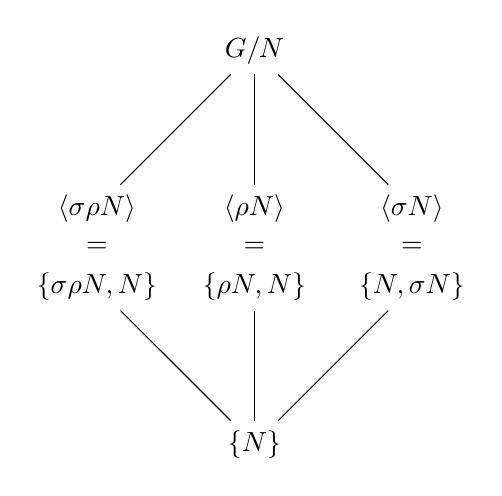
\begin{tikzpicture}
    \node (A) at (4,0) {$G/N$};
    \node (B) at (2,-2) {$\langle\sigma\rho N\rangle$};
    \node (C) at (4,-2) {$\langle\rho N\rangle$};
    \node (D) at (6,-2) {$\langle\sigma N\rangle$};
    \node (E) at (2,-3) {$\{\sigma\rho N, N\}$};
    \node (F) at (4,-3) {$\{\rho N, N\}$};
    \node (G) at (6,-3) {$\{N, \sigma N\}$};
    \node (H) at (4,-5) {$\{N\}$};
    
    \draw[-] (A) -- (B);
    \draw[-] (A) -- (C);
    \draw[-] (A) -- (D);
    \path (B)--(E) node[midway]{\storto =};
    \path (C)--(F) node[midway]{\storto =};
    \path (D)--(G) node[midway]{\storto =};
    \draw[-] (E) -- (H);
    \draw[-] (F) -- (H);
    \draw[-] (G) -- (H);
	  \end{tikzpicture}
	  \end{center}
	  \textbf{Obiettivo: studiare $S_n$}\\
	  \textbf{Ricordo:}\\
	  $X:=\{1,\ldots,n\}$\\
	  $S_n:=S_X= \{$ applicazioni biunivoche $X \rightarrow X\}$\\
	  $S_n$ gruppo di permutazioni\\
	   \textbf{Osservazione:}\\
	   $|S_n| = n!$\\
	   \textbf{Osservazione:}\\
	   se $n=3 \rightarrow |S_3| = 6$\\
	   $ \Rightarrow S_3 \cong D_3$ \\
	   \textbf{Osservazione}\\
	   $S_n\cong D_n \ \ \forall n\geq 4$\\
	   Infatti  $n! > 2n \ \ \forall n\geq 4$ 
	   \subsection{notazioni in $s_n$}\\
	   \begin{aligend*}
	   	\sigma = (1 2 3)(4 7)\\
	   	\tau = (23456)\\
		\sigma\tau=\sigma\circ\tau = (123)(46)(23456)(12)(36)(45)\\
		\tau\circ\sigma = (23456)(123)(46) = (13)(24)(56)

	   \end{aligend*}
	   \begin{lemm}
		   Data $\sigma\in S_n$ allora  $\sigma$ partizione $X = \{1,\ldots, n\}$ in sottoinsiemi permutati ciclicamente e disgiunti tra loro
	   \end{lemm}
	   \begin{dimo}
	   	Definiamo la relazione d'equivalenza $i\sim j \Leftrightarrow \exists k\in \mathbb Z \ t.c. \ \sigma^k(i) = j$\\
		È una relazione d'equivalenza!\\
		\textbf{studiamo le classi di equivalenza}\\
		fissato $i\in X$\\
		la sua clase
		 \[
			 X_i = \{\sigma^k(i)|k\in \mathbb Z\}\subseteq X
		.\] 
	quindi $\exists \ \ k_1,k_2\in \mathbb Z$ distinti t.c. $\sigma^{k_1}(i) = \sigma^{k_2}(i)$\\
	\begin{aligned*}
		\Rightarrow i = \sigma^{k_2-k_1}(i)\\
		\Rightarrow m:=min\{k\in\mathbb Z_{>0}|\sigma^k(i) = i\}\\
		\Rightarrow X_i = \{i,\sigma(i),\sigma^2(i),\ldots,\sigma^{n-1}(i)\}
	\end{aligned*}
	   \end{dimo}
	\begin{prop}
		Data $\sigma\in S_n$, allora  $\sigma$ può essere rappresentata come composizione di cicli disgiunti
	\end{prop}
	\textbf{Obiettivo:}
		Definire un omomorfismo
		\[
			sgn: S_n \rightarrow (\{\pm 1\}, \cdot)
		.\] 
		Questo ci permetterà di definire  il sottogruppo  alterno $A_n\trianglelefteq S_n$\\
		$A_n:=ker(sgn)$
		\newpage
	\begin{nota}
		Dato un polinomio\\
		$f\in \mathbb Q[x_1,\ldots, x_n]$\\
		e data $\sigma\in S_n$\\
		Definiamo
		 \[
			 f^\sigma (x_1,\ldots,x_n) := f(x_{\sigma(1),\ldots,x_{\sigma(n)\}
		.\]
		Ci sta un polinomio speciale:\\
		\begin{itemize}
			\item $\Delta (x_1,\ldots, x_n) = \prod_{1\leq i< j\leq n}(x_i - x_j)$
				\item $\Delta^\sigma (x_1,\ldots, x_n) = \prod_{1\leq i< j\leq n} (x_{\sigma (i)} - x_{\sigma (j)})$
		\end{itemize}
	\end{nota}
	\begin{defi}
		$\sigma\in S_n$\\
		$sgn(\sigma) := \frac {\Delta^\sigma}\Delta\in\{\pm 1\}$\\
	\end{defi}
		 \textbf{Osservazione}\\
		 $sgn: S_n \rightarrow \{\pm 1\}$ \\
		 è un omomorfismo\\
		 \begin{dimo}
		 	In generale\\
			$(f^\sigma)^\tau = f^{\sigma\tau}$\\
			 $(fg)^\sigma = f^\sigma g^\sigma$\\
			 $\displaystyle sgn(\sigma\tau)=\frac {\Delta^{\delta\tau}}\Delta = \frac {((\Delta^\sigma)^\tau)} \Delta = \frac {\Delta^\sigma}{\Delta} \frac {(\Delta^\sigma)^\tau}{\Delta^\sigma} = sgn(\sigma)\frac{\Delta^\tau}\Delta = sgn(\delta)sgn(\tau)$
		 \end{dimo}
		 % lezione 7
		 \subsection{Il sottogruppo alterno}

\begin{defi}
Sia $n \in \mathbb{Z}$ un intero positivo. Il \emph{sottogruppo alterno} $A_n \trianglelefteq S_n$ è definito da
\[
A_n := \{\sigma \in S_n \mid \operatorname{sgn}(\sigma) = 1 \}.
\]
Una permutazione $\sigma \in S_n$ si dice \emph{pari} se $\sigma \in A_n$ e si dice \emph{dispari} altrimenti.
\end{defi}
\textbf{Osservazione}\\
Dal momento che $\operatorname{sgn}: S_n \to \{\pm 1\}$ è un omomorfismo di gruppi per l'osservazione precedente,
abbiamo che $A_n = \ker(\operatorname{sgn}) \leq S_n$, ed è un sottogruppo normale (Esercizio passato).

\begin{prop}
Sia $n \geq 2$ un intero. Allora:
\begin{itemize}
    \item $[S_n : A_n] = 2$,
    \item $[H : A_n \cap H] = 2$ per ogni sottogruppo $H \leq S_n$ tale che $H \not\subseteq A_n$.
\end{itemize}
\end{prop}

\begin{dimo}
Chiaramente è sufficiente dimostrare la seconda parte dell'enunciato. Sia dunque $H \leq S_n$.
Due permutazioni $\sigma, \tau \in S_n$ sono congruenti modulo $A_n$ se e solo se $\sigma^{-1}\tau \in A_n$,
ovvero se e solo se
\[
\operatorname{sgn}(\sigma)\operatorname{sgn}(\tau) = 1,
\]
dove abbiamo sfruttato l'osservazione anche per dedurre $\operatorname{sgn}(\sigma^{-1}) = \operatorname{sgn}(\sigma)$.
Pertanto esistono solo due laterali sinistri dati da
\[
H \cap A_n \quad \text{e} \quad H \setminus (H \cap A_n) = \{\sigma \in S_n \mid \operatorname{sgn}(\sigma) = -1\}.
\]
\end{dimo}
\textbf{Esercizio 7.4} (Sottogruppi di $A_4$).\\ Consideriamo il sottogruppo alterno $A_4 \trianglelefteq S_4$.
\begin{enumerate}
    \item Determinare tutti gli elementi di $A_4$.
    \item Dimostrare che il sottoinsieme $V := \{\operatorname{id}, (12)(34), (13)(24), (14)(23)\} \subseteq A_4$ è un sottogruppo di $A_4$ isomorfo al gruppo di Klein $K_4$.
    \item Dimostrare che $A_4$ non contiene sottogruppi di ordine 6.
\end{enumerate}
\textbf{Soluzione.} Procediamo per passi.
\begin{enumerate}
    \item[1.] Dalla Proposizione 7.3 segue che $\lvert A_4 \rvert = 12$ poiché $\lvert S_4 \rvert = 4! = 24$. I suoi elementi sono:
    \begin{itemize}
        \item ordine 1: $\operatorname{id}$,
        \item ordine 2: $(12)(34), (13)(24), (14)(23)$,
        \item ordine 3: $(123), (132), (124), (142), (134), (143), (234), (243)$.
    \end{itemize}
    Il fatto che gli otto 3-cicli siano elementi di $A_4$ segue dall'Esercizio 6.21.

    \item[2.] Osserviamo che $V$ è chiuso rispetto all'operazione poiché
	    \begin{gather*}
    (12)(34) \cdot (13)(24) = (14)(23), \\
    (13)(24) \cdot (14)(23) = (12)(34),\\
    (14)(23) \cdot (12)(34) = (13)(24).
    \end{gather*}
    Dunque $V$ è un sottogruppo. Inoltre, gli elementi di $V$ hanno tutti ordine 1 o 2. Dalla classificazione dei gruppi di ordine 4 si ha dunque $V \cong K_4$ (si veda l'Esercizio 6.4).

    \item[3.] Dal momento che $A_4$ non contiene elementi di ordine 6 non può contenere sottogruppi isomorfi a $C_6$. Dunque un sottogruppo $H \leq A_4$ di ordine 6 è necessariamente isomorfo a $D_3$ (si veda Teorema 6.7); pertanto $H$ contiene 3 elementi di ordine 2 e due elementi di ordine 3. Ne segue che $V \subset H$, da cui l'assurdo per il Teorema 2.14 di Lagrange.
\end{enumerate}
\textbf{Esercizio 7.5} (Sottogruppi di $S_4$). Consideriamo il gruppo simmetrico $S_4$.
\begin{enumerate}
    \item[1.] Determinare il numero di sottogruppi di $S_4$ di ordine 2 e di ordine 3.
    \item[2.] Determinare tutti i sottogruppi di $S_4$ non ciclici e di ordine 4.
    \item[3.] Determinare tutti i sottogruppi di $S_4$ di ordine 6.
    \item[4.] Determinare tutti i sottogruppi di $S_4$ di ordine 8.
    \item[5.] Determinare tutti i sottogruppi di $S_4$ di ordine 12.
\end{enumerate}
\textbf{Soluzione.} Procediamo per punti.
\begin{enumerate}
	\item[1.] Ogni sottogruppo di ordine 2 è generato da un elemento di ordine 2; pertanto è sufficiente contare gli elementi di ordine 2 in $S_4$. Abbiamo: $ {4 \choose 2} = 6$ trasposizioni e i 3 elementi non banali del sottogruppo $V \subseteq A_4$ (si veda l'Esercizio 7.4). In totale esistono dunque 9 sottogruppi di ordine 2 in $S_4$.

	Ogni sottogruppo di ordine 3 è generato da un elemento di ordine 3; pertanto è sufficiente contare gli elementi di ordine 3 in $S_4$, ovvero i $3$-cicli. Questi sono $2 \cdot {4 \choose 3} = 8$, ed esistono 8 sottogruppi di ordine 3 in $S_4$.

\item[2.] Sia $H \leq S_4$ un sottogruppo non ciclico tale che $\lvert H \rvert = 4$. Ora, se $H \leq A_4$ abbiamo necessario che $H = V$, poiché $V$ contiene tutti gli elementi di $A_4$ di ordine divide 4. Se invece $H \not\leq A_4$, allora abbiamo $\lvert H \cap A_4 \rvert = 2$ per la Proposizione 7.3. Ne deduciamo che $H$ contiene un solo prodotto di trasposizioni disgiunte $(i_1 i_2)(i_3 i_4)$ con $\{i_1,i_2,i_3,i_4\} = \{1,2,3,4\}$ Ne segue necessariamente che \[H = \{ \operatorname{id}, (i_1 i_2), (i_3 i_4), (i_1 i_2)(i_3 i_4)\}.\]
	poichè il prodotto di un'altra traposizione con l'elemento $(i_1i_2)(i_3i_4)$ fornisce come risultato un $4$-ciclo. Concludiamo che i sottogruppi non ciclici di oridne $4$ di $S_4$ sono
	\[
		H_1 = \{id, (12),(34),(12)(34)\}\quad H_2 = \{id, (13),(24),(13)(24)\}
	.\] 
	\[
	H_3 = \{id, (14),(23),(14)(23)\}\quad V = \{id, (12)(34),(13)(24),(14)(23)\}
	.\] 

    \item[3.] Dal momento che $S_4$ non contiene elementi di ordine 6, non può contenere sottogruppi isomorfi a $C_6$. Dunque un sottogruppo $H \leq S_4$ di ordine 6 è necessariamente isomorfo a $D_3$ (si veda il Teorema 6.7); pertanto $H$ contiene 3 elementi di ordine 2 e 2 elementi di ordine di 3, ovvero $H$ contiene necessariamente due $3$-cicli che saranno uno l’inverso dell’altro.
Ora, ricordiamo che dall’Esercizio 7.4 segue che $A_4$ non contiene sottogruppi di ordine 6, dunque 
$\lvert H \cap A_4 \rvert = 3$ per la Proposizione 7.3. Ne deduciamo che i restanti tre elementi di ordine 2 in $H$ devono necessariamente avere segno $-1$, dunque sono trasposizioni.

Si noti infine che la scelta delle trasposizioni da inserire nel sottogruppo $H$ è univocamente determinata dai 3-cicli contenuti in $H$. Infatti, se $(i_1 i_2 i_3) \in H$ allora il prodotto 
\[
	(i_1i_4)(i_1 i_2 i_3) = (i_1 i_2 i_3 i_4)
\]
fornisce un 4-ciclo in $H$, contraddicendo il Corollario 2.15. Ne segue che se $(i_1 i_2 i_3) \in H$, allora
\[
H = \{\operatorname{id}, (i_1 i_2), (i_1 i_3), (i_2 i_3), (i_1 i_2 i_3), (i_1 i_3 i_2)\}.
\]

I sottogruppi di ordine 6 in $S_4$ sono allora:
\[
H_1 = \{\operatorname{id}, (12), (13), (23), (123), (132)\}, \quad
H_2 = \{\operatorname{id}, (12), (14), (24), (124), (142)\},
\]
\[
H_3 = \{\operatorname{id}, (13), (14), (34), (134), (143)\}, \quad
H_4 = \{\operatorname{id}, (23), (24), (34), (234), (243)\}.
\]

    \item[4.] Sia $H \leq S_4$ un sottogruppo di ordine 8. Dal momento che $8 \nmid 12$, dalla Proposizione 7.3 deduciamo che $\lvert H \cap A_4 \rvert = 4$. Dall’Esercizio 7.4 segue dunque che $V = H \cap A_4$, poiché i 3-cicli contenuti in $A_4$ hanno ordine 3 e non possono dunque appartenere ad $H$ per il Corollario 2.15.

    Supponiamo ora che $H$ contenga una trasposizione $(i_1 i_2) \in H$. Abbiamo
    \[
    (i_1 i_2)(i_1 i_2)(i_3 i_4) = (i_3 i_4) \in H,
    \]
    e
    \[
    (i_1 i_2)(i_1 i_3)(i_2 i_4) = (i_1i_3i_2i_4) \in H,
    \]
    da cui si deduce che 
    \[
    H = V \cup \{(i_1 i_2), (i_3 i_4), (i_1 i_3 i_2 i_4), (i_1 i_4 i_2 i_3)\}.
    \]

    D’altra parte, assumendo che $H$ contiene un 4-ciclo, si deduce facilmente che $H$ contiene una trasposizione e dunque $H$ è ancora della forma precedente. Concludiamo che i sottogruppi di ordine 8 di $S_4$ sono:
    \[
    H_1 = \{\operatorname{id}, (12)(34), (13)(24), (14)(23), (12), (34), (1324), (1423)\},
    \]
    \[
    H_2 = \{\operatorname{id}, (12)(34), (13)(24), (14)(23), (13), (24), (1234), (1432)\},
    \]
    \[
    H_3 = \{\operatorname{id}, (12)(34), (13)(24), (14)(23), (14), (23), (1234), (1342)\}.
    \]

    \item[5.] Sia $H \leq S_4$ un sottogruppo di ordine 12. Dalla Proposizione 7.3 deduciamo che 
    \[
    \lvert H \cap A_4 \rvert = 6 \quad \text{oppure} \quad \lvert H \cap A_4 \rvert = 12.
    \]
    Dall’Esercizio 7.4 segue dunque che $H = A_4$.
\end{enumerate}


		 %lezione 8
		 \newpage
	\subsection{Prodotto diretto tra gruppi}
	\begin{defi}
		Siano $(G_1,\cdot)$, $(G_2, *)$ gruppi il loro prodotto diretto risulta l'insieme $(G_1\times G_2)$ dotato dell'operazione:
		\[
			(g_1,g_2)\cdot(f_1,f_2) = (g_1\cdot f_1, g_2 * f_2) \ \ \forall g_1,f_1\in G_1, \ \ \forall g_2,f_2\in G_2
		.\]
		e lo indichiamo con $(G_1\times G_2)$
	\end{defi}
	\begin{prop}
		$(G_1\times G_2, \cdot)$ è un gruppo
	\end{prop}
	\begin{dimo}
		L'associatività segue da quella di $\cdot$ e  $*$ l'elemento neutro è  $(e_1,e_2)$\\
		l'inverso di $(g,f)$ con  $g\in G_1$ e $f\in G_2$ risulta $(g^{-1},f^{-1})$
	\end{dimo}
	\textbf{Esercizio}\\
	$(G_1, \cdot)$ e  $(G_2,*)$ gruppi\\
	Dimostrare:
	1) $|G_1\times G_2| = |G_1||G_2|$\\
	2) $G_1\times G_2$ è abeliano se e solo se $G_1$ e $G_2$ sono entrambi abeliani\\
	3) Dati due sottogruppi $H\leq G_1$ e $K\leq G_2 \Rightarrow H\times K\leq G_1\times G_2$ \\
	4) Dati $H\trianglelefteq G_1$ e $K\trianglelefteq G_2 \Rightarrow H\times K \trianglelefteq G_1\times G_2$ \\
	5) Dati  $H\trianglelefteq G_1$ e $K\trianglelefteq G_2$\\
	\[
		G_1/H \times G_2/H \cong \bigslant{G_1\times G_2}{H\times K}
	.\] 
	\begin{dimo}[4,5]
	\[
\begin{tikzcd}
G_1 \times G_2 \arrow[r, " \varphi"] \arrow[d] & \frac{G_1}{H} \times \frac{G_2}{K} \\
\frac{(G_1 \times G_2)}{ker \varphi} \arrow[ur, dotted, "\exists ! \bar \varphi"]
\end{tikzcd}
\]

dove 
\[
\varphi(g_1, g_2) = \left( g_1 H, g_2 K \right)
\]
	Dal primo teorema di isomorfismo
	\[
		Im \varphi \cong \frac {G_1\times G_2}{ker \varphi}
	.\] 
	$\cdot \varphi$ suriettiva poichè $\pi_H e \pi_K$ sono suriettive\\
	\begin{aligned*}
	$\cdot$ $\ ker \varphi = \{(g_1,g_2)\in G_1\times G_2| \varphi(g_1,g_2) = (H,K)\} \\= \{(g_1,g_2) | g_1H = H \ e \ g_2K = K\}$ \\
	$\{(g_1,g_2) | g_1\in H,g_2\in K\} = H\times K$
	\end{aligned*}\\
	quindi $H\times K\trianglelefteq G_1\times G_2$
	\[
		\frac{G_1\times G_2}{H\times K}\cong G_1/H\times G_2/K
	.\] 
	\end{dimo}
	\textbf{Esercizio (importante)}\\
	$(G_1,\cdot)$ e $(G_2,*)$ gruppi\\
	$H,K\normale G_1\times G_2$ tali che $H\cap K = \{\tilde e\}$ dove  $\tilde e  = (e_1,e_2)$\\
	Dimostrare che ogni elemento di $H$ commuta con ogni elemento di K.\\
	\textbf{Dimsotrazione}\\Consideriamo $h\in H, k\in K$ e verifichiamo che  $hk = kh$\\
	 \textbf{Idea:}\\
	 Dimostrare che $hkh^{-1}k^{-1} = e$\\
	 Data l'ipotesi  $H\cap K = \{e\}$ è sufficiente dimostrare che  $hkh^{-1}k^{-1}\in H\cap K$
	  \textbf{Sfruttare la normalità di H e K}\\
	  \textbf{Esercizio}\\
	  $(G_1,\cdot)$, $(G_2,*)$ gruppi
	  \[
		  H:= G_1\times \{e_2\} = \{(g,e_2)|g\in G_1\}\leq G_1\times G_2\\
	  .\] 
	  \[
		  H:= e_1\times G_2\} = \{(e_1,g)|g\in G_2\}\leq G_1\times G_2\\
	  .\] 
	  Verificare che $H$ e $K$ soddisfano le ipotesi dell'esercizio precedente
	  \begin{defi}
	  	$(G,\cdot)$ gruppo $H,K\leq G$\\
		Diremo che  $G$ è \\
		Prodotto diretto interno di $H$ e $K$ se:\\
		1) $H,K\normale G$\\
		2)  $H\cap K = \{e\}$\\
		3)  $HK = G$
	  \end{defi}
	  \begin{teo}
	  	$(G,\cdot)$ gruppo\\
		1) Se $G$ è un prodotto diretto interno di $H,K\leq G$ allora  $G\cong H\times K$\\
		2) Se  $G\cong G_1\times G_2$ allora esistono $H,K\leq G$ tali che $G$ sia prodotto diretto interno di $H$ e $K$ e inoltre $H\cong G_1, K\cong G_2$
	  \end{teo}
	  \begin{dimo}[1]
	  	$\psi: H\times K \rightarrow G$\\
		$\ \ \ \ (h,k) \rightarrow hk$\\
		Dobbiamo verificare che $\psi$ sia isomorfismo\\
		1)$\psi$ è suriettiva perchè ogni elemento di $G$ si scrive come $hk$ quindi $Im(\psi) = G$\\
		2)È anche iniettiva infatti se  $\psi(g_1,k_1) = \psi(h_2,k_1)$
		\begin{gather*}
			\Rightarrow h_1k_1 = h_2k_2\\
			\Rightarrow h_2^{-1}h_1k_1 = k_2\\
			\Rightarrow h_2^{-1}h_1 = k_2k_1^{-1}\in H\cap K = \{e\}\\
			\Rightarrow \begin{cases}
				h_2^{-1}h_1 = e\\
				k_2k_1^{-1} = e
			\end{cases} \Rightarrow (h_1,k_1) = (h_2,k_2)\\
			\Rightarrow \psi \text{ iniettiva}
		\end{gather*}\\
		Bisogna in fine dimostrare che $\psi$ è un omomorfismo, ovvero che\\
		\[
		\psi(h_1h_2,k_1k_2) = \psi(h_1,k_1)\psi(h_2,k_2)
		.\] 
		dunque
		\[
		\psi(h_1h_2,k_1k_2) = h_1h_2k_1k_2 = h_1(h_2k_1)k_2 = h_1(k_1h_2)k_2 = \psi(h_1,k_1)\psi(h_2,k_2)
		.\] 
		Ricordando che tutti gli elementi di $H$ commutano con quelli di $K$
	  \end{dimo}
	  \begin{dimo}[2]
	  	Per ipotesi esiste un isomorfismo
		$ \varphi: G_1\times G_2 \rightarrow G$\\
		$\ \ \ (g_1,g_2) \rightarrow \varphi(g_1,g_2)$\\
		considero\\
		$H:= \varphi(G_1,\{e_2\})$\\
		$K:= \varphi(\{e_1\}\times G_2)$ \\
		Abbiamo visto che\\
		$\cdot G_1\times \{e_2\}\trianglelefteq G_1\times G_2 \rightarrow H\normale G$\\
		$\cdot \{e_1\}\times G_2\normale G_1\times G_2 \rightarrow K\normale G$ \\
		\[
			H\cap K = \varphi((G_1\times\{e_2\})\cap(\{e_1\}\times G_2)) = \{e\}
		.\] \\
		\[
			HK = \varphi((G_1\times \{e_2\})(\{e_1\}\times G_2)) = G
	.\]
	Le opportune restrizioni di $ \varphi$ forniscono gli isomorfismi
	\[
		H\cong G_1\times \{e_2\}\cong G_1
	.\] 
	\[
		K\cong \{e_1\}\times G_2\cong G_2
	.\] 

	  \end{dimo}
\textbf{Esempio:}\\
Siano $n,m\in\mathbb Z_{>0}$ t.c.\\
$MCD(n,m) = 1$\\
Consideriamo  $C_{nm} = <p>$\\
dove  $ord(p) = nm$\\
Considero
 \[
H = <\rho^m> \ \ \ K = <\rho^n>
.\] 
$|H| = ord(\rho^m) = n$\\
$|K| = ord(\rho^n) = m$\\
Verifichiamo che
 \[
	 C_{nm} \cong H\times K
.\] 
Dobbiamo mostrare:
\begin{enumerate}
	\item $H,K\normlae C_{nm}$\\
	\item $H\cap K = \{Id\}$\\
	\item $HK = C_{nm}$
	
\end{enumerate}\\
1) $C_{nm}$ abeliano, quindi $H,K\nomrale C_{nm}$\\
2) $H\cap K = ?$\\
sia $\rho^h\in H\cap K$\\
Allora
 \[
\begin{cases}
	\rho^h = (\rho^m)^{t_1}\\
	\rho^h = (\rho^h)^{t_2}
\end{cases} \ \ \ \ \ \begin{cases}
	m|h\\
	n|h
\end{cases}
.\] 
Ma $h\geq mcm(m,n) = mn \Rightarrow  h = mn \Rightarrow \rho^h = Id \Rightarrow H\cap K = \{Id\}$
\[
	|HK| = \frac{|H||K|}{|H\cap K|} = \frac {nm}1
.\] 
$ \Rightarrow HK$ è tutto chiuso quindi è $C_{nm}$\\
\begin{defi}[Automorfismo]
	$(G,\cdot)$ gruppo\\
	Un automorfismo di $G$ è un isomorfismo  $ \varphi:G \rightarrow G$
\end{defi}
\textbf{Osservazione}\\
$(G,\cdot)$ gruppo\\
$ \Rightarrow Aut(G) = \{\text{automorfismi di } G\}\\$
è un gruppo (rispetto alla composizione)\\
\textbf{Esempio:}\\
$(G,\cdot)$ gruppo\\
Fissato $g\in G$ definiamo\\
 \begin{aligned}
	 I_g: &G \rightarrow G\\
	      &f \rightarrow gfg^{-1}
\end{aligned}\\
$I_g$ si dice automorfismo interno\\
$Int(G) = \{\text{automorfismi interni di } G\}$ \\
\begin{prop}
	$Int(G)\normale Aut(G)$
\end{prop}
\begin{dimo}
	$If_G = I_e\in Int(G)$\\
	dato  $g\in G$ allora\\
	\[
		I_{g^{-1}} = I_g^{-1} \rightarrow \begin{cases}
			I_g\in Aut(G)\\
			Int(G) \text{ è chiuso rispetto agli inversi}
		\end{cases}
	.\] 
	$I_{g_2}\cdot I_{g_1}(f) = g_3g_2fg_2^{-1}g_2^{-1}
	= (g_2 g_1)f(g_2g_1)^{-1} = I_{g_2g_1}(f)$\\
	$I_{g_2}\cdot I_{g_1} = I_{g_2g_1}$\\
	quindi $Int(G)$ è chiuso rispetto alla composizione\\
	Quindi $Int(G)\leq Aut(G)$\\
	Basta verificare che:\\
	$ \varphi\circ Int(G)\circ \varphi^{-1}\subseteq Int(G)  \ \ \forall \varphi\in Aut(G)$\\
	ovvero dato $g\in G$\\
	 \[
		 \varphi\circ I_g\circ \varphi^{-1}\in Int(G)
	.\] 
	$\forall f\in G$\\
	\begin{aligend}
		 &\varphi\circ I_g \circ \varphi^{-1}(f) = \varphi(g \varphi^{-1}(f) g^{-1}) = \\
		 &\varphi(g) \varphi( \varphi^{-1}(f)) \varphi(g^{-1}) = \\
		 &= \varphi(g) f \varphi(g) =\\
		 & = I_{ \varphi(g)}(f)\\
		 &\Rightarrow \varphi\circ I_g \circ \varphi^{-1} = I_{ \varphi(g)}\in Int(G)
	\end{aligend}
\end{dimo}
\begin{defi}[Centro di un gruppo]
	$(G,\cdot)$ gruppo\\
	Il centro di $G$ è 
	\[
		Z(G):=\{g\in G| gf = fg \ \ \forall f\in G\}
	.\] 
\end{defi}
	\textbf{Osservazione}\\
	$Z(G)\normale G$\\
	 \textbf{Osservazione:}\\
	 $(G,\cdot)$ gruppo\\
	 Definiamo un omomorfismo\\
	 \begin{aligned}
		 \varphi: \ &G \rightarrow Int(G)\\
			& g \rightarrow I_g
	 \end{aligned}\\
		 \cdot $ \varphi$ è suriettiva\\
		 \cdot $ \varphi$ è omomorfismo\\
	 $ \varphi(g_2g_1)= \varphi(g_2) \varphi(g_1)$\\
	 $I_{g_2g_1} = I_{g_2}\circ I_{g_1}$\\
	 Chi è il $ker( \varphi)$\\
	 \begin{aligned}
		 ker( \varphi) &=  \{ g\in G | \varphi(g) = Id\} = \\
				 &= \{ g\in G | I_g = Id\} = \\
				 & = \{g\in G | \forall f\in G : I_g(f) = Id(f)\} = \\
				 & = \{g\in G | \forall f\in G : gfg^{-1} = f \} = Z (G)
	 \end{aligned}\\
	 Dal I teorema di isomorfismo si ha che
	 \[
	 Int(G) \cong G/Z(G)
	 .\] 
	 \subsection{Prodotto semidiretto}\\
	 Consideriamo due gruppi\\
	 $(N,\cdot)$ e $(H,*)$\\
	 Fissiamo un omomorfismo\\
	  \begin{aligned}
		  \phi: &H \rightarrow Aut(N)\\
			& h \rightarrow \o_n
	 \end{aligned}
	 \begin{defi}[Prodotto semidiretto]
	il prodotto semidiretto di $N$ e $H$ tramite $\o$ è l'insieme $N\times H$ dotato dell'operazione
	 \[
		 (n_1,h_1)\cdot (n_2,h_{2}) = (n_1\cdot \o_{h_1}(n_2), h_1*h_2)
	.\] 
	$\forall n_1,n_2\in N \ \ \ \ \forall h_1,h_2\in H$
\end{defi}
\begin{nota}
Indichiamo il prodotto semidiretto tra $N$ e $H$ con il simbolo $N\rtimes_{\o}$$H$
\end{nota}
\begin{prop}
	$N\rtimes_{\o} H$ è un gruppo
\end{prop}
\begin{dimo}
	Dato $(n,h)\in N\rtimes_{\o} H$\\
	l'inverso è dato da  $(\o_{h^{-1}}(n^{-1}),h^{-1})$
\end{dimo}
\newpage
\begin{defi}
	$(G,\cdot)$ gruppo\\
	$N,H\leq G$ Diremo che\\
	 $G$ è prodotto semidiretto interno di $N$ e $H$ se\\
	 \begin{itemize}[noitemsep]
		 \item $N\normale G$\\
		 \item $N\cap H = \{e\}$\\
		 \item $NH = G$
	 \end{itemize}
\end{defi}
\textbf{Esempio}\\
$D_n = <\rho, \sigma> \ \ N = <\rho> \normale D_n$\\
 $ H = <\sigma > \leq D_n$. Allora $D_n$ è prodotto semidiretto interno di $N$ e $H$\\
\textbf{Osservazione:}\\
$h_1\in H, \ \ \o_{h_1}\in Aut(N) \ \ \o_{h_1}(n_2)\in N$\\
\textbf{Esempio}\\
Scegliendo\\
\begin{aligned}
	\o : &H \rightarrow Aut(N)\\
	     & h \rightarrow \o_h
\end{aligned}\\
con $\o_n := Id_N \ \ \forall h\in H$\\
Abbiamo:
 \[
	 (n_1,h_1)\cdot (n_2,h_2) = (n_1\cdot n_2, h_1 * h_2)
.\] 
Quindi il prodotto diretto è un caso particolare del prodotto semidiretto

\subsection{Prodotto semidiretto interno:}
Un gruppo \( G \) si dice \textit{prodotto semidiretto interno} di \( N \) e \( H \leq G \) se:
\begin{enumerate}
    \item \( N \trianglelefteq G \),
    \item \( N \cap H = \{ e \} \),
    \item \( N H = G \).
\end{enumerate}
\textbf{Esercizio}\\
Sia $\o : H \rightarrow Aut(N)$ un omomorfismo\\
Dimostrare:\\
$1) |N\rtimes_{\o} H | = |N||H|$\\
$2) N\rtimes_{\o} H$ è abeliano $ \Leftrightarrow N,H$ abeliani \\
$3) \tilde H \leq H, \tilde N \leq N$ (sottogruppo caratteristico)\\
 \[
\tilde N \semi \tilde H := \{ (n,h)\in N\semi H | 
	n\in \tilde N,
	n\in \tilde H
 \}
.\] 
è un sottogruppo di $N \semi H$\\
\begin{defi}[Sottogruppo caratteristico]
	$\tilde N\leq N$ sottogruppo caratteristico se \\$ \varphi(n)\in \tilde N\ \ \forall n\in \rilde N\ \ \ \forall \varphi\in Aut(N)$
\end{defi}
\begin{teo}
Sia \( G \) un gruppo. \\1) Se \( G \) è prodotto semidiretto di \( N \) e \( H \leq G \), allora esiste un omomorfismo \( \o : H \to \text{Aut}(N) \) tale che $G\cong N\semi H$\\
2) Se  $G\cong \tilde N\semi \tilde H$ allora esistono $N,h\leq G$ t.c.
\begin{itemize}
	\setlength\itemsep{-1em}
	\item $G$ sia prodotto semidiretto interno di $N$ e $H$ \\
	\item $N\cong \tilde N, h\cong \tilde H$
\end{itemize}
\end{teo}
\begin{dimo}[1]
	Definiamo l'applicazione\\
	\begin{aligned}
		\o :& H \rightarrow Aut(N)\\
		    &	h \rightarrow \o_n
	\end{aligned}\\
	dove $\o_{h}(n) := (hnh^{-1})\in hNh^{-1} = N \ \ \forall n\in N$\\
	Dato che abbiamo assunto  $N$ normale\\
	Abbiamo verificato la volta scorsa che è un omomorfismo.\\
	Definiamo l'applicazione\\
	\begin{aligned}
		\psi: &N\semi H \rightarrow G\\
		      &(n,h) \rightarrow nh
	\end{aligned}\\
	$\psi$ è suriettiva poiché $N\cdot H = G$ \\
	$\psi$ è iniettiva poichè\\
	\begin{gather*}
		n_1h_1 = n_2h_2 \rightarrow n_2^{-1}h_1 = h_2h_1^{-1}\in H\cap N = \{e\}\\ 
		\Rightarrow \begin{cases}
			n_2^{-1} n_1 = e\\
			h_2h_1^{-1} = e
		\end{cases} \rightarrow (n_1,h_1) = (n_2,h_2)
	\end{gather*}
	\textbf{$\psi$ è omomorfismo:}\\
	\begin{aligned}
	&\psi((n_1,h_1)\cdot(n_2,h_2)) =\\
	&=\psi((n_1\o_{h_1}(n_2),h_1h_2))\\
	& =n_1\o_{h_1}(n_2)h_1h_2\\ 
	&= n_1h_1n_2h^{-1}_1h_1h_2 = \psi(n_1,h_1)\cdot\psi(n_2,h_2)
		
	\end{aligned}\\
	Omomorfismo biunivoco
\end{dimo}
\newpage
	\begin{dimo}[2]
		Dato un isomorfismo\\
		$\psi :\tilde N\semi\tilde H \rightarrow G $\\
		definiamo:\\
		$N := \psi (\tilde N\semi \{e_{\tilde H}\})\normale G$\\
		$H:=\psi(\{e_n\}\semi \tilde H)$\\
		Osserviamo che:\\
		$\cdot \tilde N \cong \tilde N\semi \{e_{\tilde H}\}\cong N$\\ $\cdot \tilde H\cong \{e_{\tilde H\}\semi \tilde H\cong H$\\
			$\cdot N\cap H = \{e\}$\\
			 $\cdot NH = e$ \\(analogo alla dimostrazione per prodtto diretto)
	\end{dimo}
	\section{Numeri primi e aritmetica}
	\begin{defi}[Numero primo]
		Un intero $\rho > 1$ si dice primo se  $\forall a,b\mathbb Z$
		 \[
			 \rho|ab \rightarrow \rho|a \text{ oppure } \rho|b
		.\] 
	\end{defi}
	\begin{defi}[Numero irriducibile]
		Un intero $\rho>1$ si dice irriducibile se i suoi unici divisori positivi\\ sono  $1$ e $\rho$
	\end{defi}
	\textbf{Esercizio:}\\
	Dimostrare che $\rho$ è primo $\Leftrightarrow$ è irriducibile
	\begin{teo}[Fondamentale dell'aritmetica]
		$n>1$ intero. Allora $n$ si scrive in modo unico come
		\[
			n = \rho_1^{k_1}\cdot\ldots\cdot \rho_r^{k_r} \ \ \ \ \ \text{ (forma canonica)}
		\] 
		dove $k_i>0 \ \ \forall i\in\{1,\ldots,r\}$\\
		e $\rho_1<\rho_2<\ldots<\rho_r$\\
		e $\rho_i$ è primo  $\forall i\in \{1,\ldots,r\}$
	\end{teo}
	\begin{teo}
		$\rho$ primo. Allora\\
		$\sqrt \rho $ è irrazionale (ovvero $\sqrt\rho\ni \mathbb Q$)
	\end{teo}
	\begin{dimo}[Per assurdo]
		$\exists a, b\in \mathbb Z$ t.c.  $\sqrt\rho = \frac a b$ con $MCD(a,b) = 1$\\
		Allora:\\
		 $(a) + (b) = (MCD(a,b)) = (1)$\\
		  $\rightarrow 1\in (a)) + (b)\\
		  \exists r,s,\in\mathbb,$ t.c. $1 = ra + sb$ (identità di Bezout)\\
		  ora:  $ \begin{cases}
		  	a = \sqrt \rho b \\ b\rho = a\sqrt\rho
		  \end{cases}$ \\
		  Quindi:
		  $\sqrt \rho = \rho\cdot 1 = \sqrt \rho\cdot (ra + sb)\\
		  (\sqrt\rho a)r + (\sqrt\rho b)s$\\
		  =  $\rho b r + as\in \mathbb Z$\\
		   $ \Rightarrow \sqrt\rho\in\mathbb Z$ quindi $\sqrt\rho$ è un intero che divide $\rho$ e $1<\sqrt\rho<\rho$
	\end{dimo}
	\begin{teo}[Euclide]
		Esistono infiniti numeri primi
	\end{teo}
	\begin{dimo}
		Supponiamo per assurdo che $\exists$ un numero finito di primi $\rho_1,\ldots, \rho_r$\\
		Definiamo:
		$N:= (\rho_1 \cdot\ldots\cdot\rho_r) + 1 > 1$\\
		$ \Rightarrow\exists \rho_k$ primo tale che $\rho_k | N$\\
		 $ \Rightarrow \begin{cases}
		 	\rho_k|N\\
			\rho_k|N-1
		 \end{cases} \Rightarrow \rho_k|N-(N-1) \Rightarrow \rho_k | 1$, assurdo
	\end{dimo}
	\begin{defi}[Primi di Euclide]
		Sia $\rho$ primo
		\[
			\rho^\# := \left(\prod_{q\in\rho, q \text{ primo}} q \right) + 1
		.\] 
		$\rho^\#+1$ si dice numero di Euclide
	\end{defi}
	\textbf{Congettura}\\
	Esistono infiniti primi di euclide

\subsection{Svolgimento esercizi}
	\textbf{Ossercazione:}\\
	Quali sono gli elementi di oridne $21$ in $S_{13}$?\\
	Ricordo che in $S_4$, gli elementi $(12)(34), (13)(24), (14)(23)$ hanno ordine 2\\
	gli elementi di ordine 21 sono $(3-ciclo)(7-ciclo)$ sono $\frac {13!}{126}$\\
	$(3-ciclo)(3-ciclo)(7-ciclo)$ sono  $\frac{13!}{126}$ \\
	Nelle note del corso trovi soluzioni degli esercizi\\
	%TODO aggiugni la roba
	\textbf{Esercizi:}\\
	1) $(\Z, +)\ \ \ Aut(\Z) = ?$ \\
	\textbf{Osservazione}\\
	Per definire un omomorfismo è sufficiente definirlo sui generatori.\\
	Se inoltre vogliamo un automorfismo $ \phi(1)$ deve generare $\Z \Rightarrow  \phi(1) = 1 $ o $-1$\\
	$ \Rightarrow Aut(\Z) = \{Id, -Id\}\cong C_2$ \\
	2) Dimostrare che $D_n\cong C_n\semi C_2$ dovea\\  \begin{aligned}
		\phi: &C_2 \rightarrow Aut(C_n)  = <\rho> \ \ \text{ e } \phi(\rho) = \rho^{-1}\\
		      &\sigma \rightarrow\phi_\sigma
	\end{aligned}
SOluzione:\\
$N = <\rho> \normale D_n \hfill [D_n:N] = 2$\\
 $H:= <\sigma>\leq D_n$\\
 Verifichiamo che  $D_n$ è prodotto semidiretto interno di $N$ e $H$\\
 $\cdot N\cap H = \{Id\}$\\
 $\cdot |NH| = \frac {|N||H|}{|N\cap H|} = 2n \Rightarrow  NH =  D_n$ \\
 Ora dal teorema segue che $D_n = N\semi H$\\
 dove  \begin{aligned}
	 \phi: &H \rightarrow Aut(N)\hfill H = \{Id,\sigma\}\\ 
	       &h \rightarrow h
 \end{aligned}\\
 $\cdot\phi_{Id} = Id_N$\\
 $\cdot_\sigma(\rho) = \sigma\rho\sigma^{-1} = \sigma\rho\sigma = \sigma\sigma\rho^{n-1} = p^{n-1} = p^{-1}$\\
 dove abbiamo usato il fatto che $\rho^i\sigma = \sigma\rho^{n-i}$\\
 Infine  $H\cong C_2 \ \ N\cong C_n$\\
 \textbf{Osservazione}\\
 Se avessimo scelto  \begin{aligned}
	 \phi: &C_2 \rightarrow Aut(C_n)\\
	       &\sigma \rightarrow \phi_\sigma
 \end{aligned}\\
 con $\phi_\sigma (\rho) = \rho$ Avremmo  $C_n\semi C_2= C_n\times C_2$ è abeliano $ \Rightarrow $ non isomorfo a $D_n \ \ \forall n\geq 3$\\
  $3) G = C_5\cong \Z/(5) \ \\ \ Aut(C_5)$\\
  Cerchiamo le immagini di $ \varphi(\rho)$\\
  $\Z/(5) = \{[0],[1],[2],[3],[4]\}$ ricordo che  $ord_{\Z/(n)}([a]) = \frac {n}{MCD(a,n)}$\\
  $ ord([1]) = ord([2]) = ord([3]) = ord([4])$\\
  $ord([0]) = 1 \Rightarrow |Aut(\Z/(5))| = 4$ \\
  \textbf{Osservazione} \\
  In generale denotiamo con $U_n$ il gruppo delle classi in  $\Z/(n) \ \ U_n = \{[a]\in\Z/(n) | MCD(a,n) = 1\}$\\
  \textbf{Esercizio}\\
  $U_n$ è un gruppo rispetto \begin{aligned}
	  U_n&\times U_n \rightarrow U_n\\
	  ([a&],[b]) \rightarrow[a\cdot b]
  \end{aligned}\\
  Si dice gruppo degli invertibili\\
  \textbf{Esercizi}|\
  $\cdot Aut(C_n) \cong U_n$\\
   $\cdot Aut(K_4) = S_3$\\
   \begin{teo}[Cinese del resto]
	   $C_{nm}\cong C_n\times C_m$ per ogni coppia di interi tale che  $MCD(m,n) = 1$
\end{teo}
\begin{dimo}
	Già dimostrato
\end{dimo}
\begin{teo}[Piccolo teorema di Fermat]
	$p$ primo, $a\geq 1$  $MCD(a,p) = 1 \Rightarrow a^{p-1}\equiv_p 1$
\end{teo}
\begin{dimo}
	$A:=\{a,2a,3a,\ldots,(p-1)a\}$ sono $p-1$ interi.\\
	Mi chiedo se $[ra] = [sa]$ in $\Z/(p)$\\
	Sappiamo che esistono  $1\leq r < s \leq p-1$ tali che  $[ra] = [sa]$ in $\Z/(p) \Rightarrow $ Assurdo poiché \\
	$[r]\neq [s]$ in $\Z/(p)$\\
	Quindi le classi  definite dagli elementi di $A$ sono tutte distinte e non banali $ \Rightarrow $ $\{[a],[2a], \ldots, [(p-1)a]\} = \{[1],[2],\ldots,[p-1]\}$\\
	Consideriamo il prodotto  $a\cdot 2a\cdot\ldots\cdot (p-1)a\eqiuv_p 1\cdot 2 \cdot 3 \cdot \ldots \cdot (p-1)$\\
	$ \Rightarrow a^{p-1}(p-1)!\equiv_p (p-1)$ Dato che $MCD(p,(p_1)) = 1$ abbiamo $a^{p-1}\equiv_p 1$
\end{dimo}
	 \begin{coro}
		$a\geq 1 $ p primo $ \Rightarrow a^p \equiv_p a$ \\
	\end{coro}
	\begin{dimo}
		Se $MCD(a,p) = 1 $ segue dal piccolo teorema di Fermat\\
		$\cdot$ Se  $MCD(a,p)\neq 1 \ \Rightarrow  \ p|a \Rightarrow [a] = [0] $  in $\Z/(p) \Rightarrow a^p\equiv_p 0\equiv_p a$ \\
	\end{dimo}
	\textbf{Obbiettivo}\\
	Cosa succede al piccolo teorema di Fermat senza $p$ primo?
	\begin{defi}[Funzione di Eulero]
		$n\geq 1 \Rightarrow \phi(n) = |U_n|$ ovvero $\phi(n)$ è il numero di interi positivi minori o uguali ad  $n$ coprimi con $n$
	\end{defi}
	\textbf{Esempio}\\
	$p$ primo $ \Rightarrow $  $\phi(p) = p-1$;  $\phi (1) = 1$\\
	 \textbf{Esercizio}\\
	 Mostrare che se $ p $ è primo $ \Rightarrow  \phi (p^k) = p^k - p^{k-1} = p^{k-1}(p-1)$ \\
	 \textbf{Soluzione:}\\
	 $MCD(a,p) = 1 \Leftrightarrow p | a$ Quindi gli elementi inclusi sono $p,2p,3p,\ldots, (p^{k-1})p $ tutti i multipli di $p \leq p^k$\\
	 Sono  $ p^{k-1}$ elementi $ \Rightarrow \phi (p^k) = p^k - p^{k-1}$ \\
	 \newpage
	 \begin{defi}
		 Una funzione $f:\Z_{>0} \rightarrow\Z$ si dice moltiplicativa se $f(n\cdot m) = f(n)\cdot f(m)$ se $MCD(n,m) = 1$
	 \end{defi}
	 \textbf{Obiettivo}\\
	 Dimostrare che $\phi$ è moltiplicativa\\
	 \textbf{Esercizio}\\
	 $a,b,c\in \Z$\\
	  $MCD(a,b,c) = 1 \Leftrightarrow \begin{cases}
	  	MCD(a,b) = 1\\
		MCD(a,c) = 1
	  \end{cases}$
	  \begin{teo}[Eulero]
		  $\phi : \Z_{>0} \rightarrow \Z$ di Eulero è moltiplicativa
	  \end{teo}
	  \begin{dimo}
	  	Per il teorema cinese del resto se $MCD(n,m) = 1 \Rightarrow  $\\ \begin{aligned}
			$\psi : &\Z/(nm) \rightarrow\Z(n)\times \Z(m)\\
				&[a]_{nm} \rightarrow([a]_n,[a]_m)$
	  	\end{aligned}
		Consideriamo la restrizione $\psi|_{U_{nm}}:U_{nm} \rightarrow Z/(n)\times \Z/(m)$ è una funzione iniettiva\\
		Studiamo $Im(\psi|_{U_{nm}}) = U_n\times U_m$\hfill (esercizio)\\
		$ \Rightarrow |U_{nm}| = |U_n|\times |U_m| \Rightarrow \phi(nm) = \phi(n)\phi(m)$
	  \end{dimo}
	  \textbf{Osservazione} (Formula generale)\\
	  	$n>1$ intero con fattorizzazione canonica
		\[
			n = p_1^{k_1}\cdot\ldots\cdot p_r^{k_r} \Rightarrow \phi(n) = \phi(p_1^{k_1})\cdot\ldots\cdot\phi(p_r^{k_r})
		\]
	\[
		= (p_1^k_1- p_1^{k_1-1})\cdot\ldots\cdot(p_r^{k_r}-p_r^{k_r-1}) = \left(1-\frac {1}{p_1^{k_1}} \right) \cdot\ldots\cdot \left(1 - \frac {1}{p^{k_r}_r} \right)
		.\] 
		\textbf{Osservazione}\\
		$|Aut(C_n)| = \phi(n)$ dato che  $Aut(\Z/(n))\cong U_n$\\
		 \textbf{Osservazione}\\
		 Se $n\geq 2 \Rightarrow \phi(n)$ è pari\\
		 \begin{itemize}
			 \item Se $ n= 2^k \Rightarrow \phi(n) = 2^k - 2^{k-1} = 2^{k-1}$
			 \item $n > 2 \Rightarrow k > 1 \Rightarrow k-1 > 0 \Rightarrow 2 | \phi(n)$ 
			 \item Se $n\neq 2^k \Rightarrow \exists p$ primo e dispari tale che $p | n \Rightarrow n = p_1^{k_1}\cdot\ldots\cdot p_r^{k_r}$  con $p = p_j$ per qualche  $j\leq r \Rightarrow \phi(p_j^{k_j})|\phi(n)$. Ma $\phi(p_j^{k_j})= p^{k_j}-p^{k_j-1} = p^{k_j-1}(p-1)$\\
				 $ \Rightarrow (p_j - 1) | \phi (p_j^{k_j}). $Ma $p_j$ è dispari $ \Rightarrow 2 | (p_j-1) \Rightarrow 2 | \phi(n)$
		 	
		 \end{itemize}
		 \begin{teo}[Waring 1770, Lagrange 1771]
		 	Se $p$ è un numero primo $  \Rightarrow (p-1)! \equiv_p (p-1)$\\
		 \end{teo}
\begin{dimo}
	Studiare le soluzioni di $x^2 - 1 \equiv_p 0$\\
	$(x^2-1)\equiv_p (x-1)(x+1)\equiv_p 0$\\
	Quindi $x-1\equiv_p 0$ oppure  $x + 1\equiv_p 0$\\
	ovvero deduciamo che gli unici elementi in  $U_p$ di ordine $\leq 2 $ sono $[1]$ e $[p-1]$\\
	Nel prodotto  $[(p-1)!]$ compaiono tutti gli elementi di $U_p \Rightarrow $   ogni elemento di $U_p$ diverso da  $1$ e $p-1$ oppure con il suo inverso ("moltiplicativo")
\end{dimo}
\subsection{funzione di Eulero}



	%lezione successiv
	$\phi: \mathbb Z_{>0} \rightarrow \mathbb Z$\\
	$\text{} \ \ \ \ n \rightarrow |U_n|$\\
	\textbf{Ricordo:}\\
	$\phi(1) = 1$\\
	 $\phi(\rho) = \rho -1$\\
	 $\phi(\rho^k) = \rho^k - \rho ^{k-1}$\\
	 $\phi(n\cdot m) = \phi(n)\phi(m)$\ \ \ \ se  $MCD(n,m) = 1$\\
	  \begin{lemm}
	 	$n>1, a\in\Z$ t.c.  $MCD(n,a) = 1$\\
		sia  $\{a_1,\ldots,a_{\phi(n)}\}$ l'insieme dei numeri positivi minori di $n$ coprimi con n distinti fra loro.\\
		Allora $\{[a_1],\ldots,[a_{\phi(n)}] = \{[aa_1],\ldots, [aa_{\phi(n)}]\}$ (Classi in $Z/(n)$)
	 \end{lemm}
	 \begin{dimo}
		 Basta verificare che gli elementi delle classi $[aa_i] \ \ \forall \ 0<i<\phi(n)$\\
		 Siano tutte distinte tra loro e  $aa_i$ sia coprimo con n  $\forall \ 0<i<\phi(n)$ \\
		 Se per assurdo $[aa_i] = [aa_j] \ \ i\neq j \Rightarrow aa_i\equiv aa_j\  mod(n) \Rightarrow a\equiv a_j \ mod(n)$ Assurdo perché $1\leq a_i, a_j< n$ per ipotesi e dunque  $a_i-a_j\not\in (n)$\\
		 \begin{cases}
		  $MCD(a,n) = 1 \\ MCD(a_i,n) = 1$
		 \end{cases} $\Rightarrow MCD(a,a_i) = 1\\$
	 \end{dimo}
	 \begin{teo}[Eulero 1760]
	 	$n>1 ,a\in\Z$ tale che $MCD(a,n) = 1$\\
		Allora
		 \[
			 a^{\phi(n)}\equiv 1\  mod(n)
		.\] 
	 \end{teo}
	 \textbf{Nota}\\
	 Se $n$ è primo ritroviamo il piccolo teorema di Fermat
	 \begin{dimo}
	 	Considero la situazione del lemma:\\
		$A = \{a_1,\ldots,a_{\phi(n)}\}$\\
			Insieme degli interi positivi minori di n e coprimi con n distinti tra loro\\
			Dal lemma segue che
			\[
				a_1\cdot\ldots\cdot a_{\phi(n)}\equiv (aa_1)\cdot\ldots\cdot (aa_{\phi(n)}) \ mod(n)
			.\] 
			\[
				\equiv a^{\phi(n)}\cdot a_1\cdot\ldots\cdot a_{\phi(n)} \ mod(n)
			.\] 
			Dal momento che $MCD(a_i,n) = 1$\\
			abbiamo:  $1\equiv a^{\phi(n)}\ mod(n)$
	 \end{dimo}
	 \textbf{Esempio}\\
	 Se volessi calcolare le ultime $3$ cifre di $2024^{2025}$ Studiamo la congruenza  \[x\equiv 2024^{2025} \ mod(1000)\]
	 È equivalente al sistema (Teorema cinese del resto):\[
	 \begin{cases}
	 x\equiv 2024^{2025} \ mod(2^3)\\
	 x\equiv 2024^{2025} \ mod(5^3)
 \end{cases}\]
 Alternativamente mi accorgo che la prima equazione è equivalente a
 \[
	 x\equiv 24^{2025} \ mod(1000)
 .\] 
 $\phi(1000) = \phi(2^3)\phi(5^3) = (2^3 - 2^2)(5^3-5^2) = 400$\\
 $ \Rightarrow 24^{400} \equiv 1 mod(n)$\\
 Ma questo implica che la congruenza che devo studiare è:
 \[
 \Rightarrow x\equiv 24^{2025} mod(1000)
 .\] 
 \[
 \Rightarrow \begin{cases}
	 x\equiv 24^{2025}\ mod(8)\\
	 x\equiv 24^{2025}\ mod(125)
 \end{cases} \Rightarrow \begin{cases}
 	x\equiv 0\ mod(8)\\
	x\equiv 24^{2025} \ mod(125)
 \end{cases}
 .\] 
 Dove nell'ultimo passaggio abbiamo utilizzato il fatto che $8|24$ e $24^{\phi(125)}\equiv 24^{100}\equiv 1\ mod(125)$\\
 Alla fine dovremmo ricostruire la soluzione in $\Z/(1000)$ che sarà unica per il teorema cinese del resto\newpage
 \subsection{Teorema cinese del resto}
 \textbf{Problema}\\
 Dato un sistema di congruenze\\
 \begin{cases}
 	x\equiv = a_1\ mod(n_1)\\
	\vdots\\
	x\equiv = a_r\ mod(n_r)\\
 \end{cases}\\
 con $MCD(n_i,n_j) = 1 \ \ \forall i\neq j$  \\
 Come ricostruire l'unica soluzione $[\bar x]\in \Z/(n_1\cdot\ldots\cdot n_r)$\\ $\bar x\equiv a_i\ mod(n_i)\ \forall i\in \{1,\ldots,r\}
  $\\
  \textbf{Idea}\\
  Definiamo:\\
  $n: = n_1\cdot n_r$\\
  $N_i := \frac n {n_i}$\\
  $\bar  x := a_1N_1^{\phi(n_1)} + \ldots + a_rN_r^{\phi(n_r)}$\\
  Ora $\bar x\equiv a_i N^{\phi(n)}\ mod(n) \Rightarrow \bar x = a_i mod(n_i) \ \ \forall i$ 
  \begin{teo}[TCR]
	Dato il sistema\\
	\begin{cases}
		x\equiv a_1 \ mod(n)\\
		\ldots\ome
		x\equiv a_r \ mod(n_r)\\
	\end{cases}\\
	con $MCD(n_i,n_j) = 1 \ \ \forall i\neq j$\\
	Allora esiste un'unica classe  $[\bar x]\in \Z/(n_1\cdot\ldots\cdot n_r)$ tale che\\
	$\bar x\equiv a_i\ mod(n_i) \ \ \forall i\in \{1,\ldots, r\}$\\
\end{teo}
	\begin{dimo}[Alternativa al teorema di Eulero]
		$n:= n_1\codt\ldots\cdot n_r$\\
		$N_i = \frac n {n_i}$\\
		$\bar x :=  a_1N_1m_1+\ldots a_rN_rm_r\\$
		dove gli $m_i$ sono univocamente determinati dalla condizione
		$N_im_i\equiv 1 mod(n_i)$\\
		Infatti  \[
		\bar x\equiv a_iN_im_i \ mod(n_i) \Rightarrow \bar x\equiv a_i mod(n_i)
		.\] 
		Osserviamo che $MCD(N_i,n_i) = 1$ Per ipotesi\\
		Quindi $[N_i]\in U_{n_i}$ e  $[m_i]$ è l'unico inverso di $[N_i]$ in  $U_{n_i}$
	\end{dimo}
	\textbf{Osservazione}\\
	Per risolvere i sistemi di congruenze "basta" saper trovare gli inversi degli elementi in gruppi $U_{n_i}$\\
	 \textbf{Esercizi dalle schede}\\
	 \textbf{Esercizio (Gauss)}\\
	 Dato un intero $n > 1$ dimostrare che  $n = \sum_{d | n} \phi (d)$ (somma di tutti i divisori positivi di $n$
\begin{dimo}
	$S_d : = \{m\in \Z | MCD(m,n) = d, 1 \leq m\leq n\}$\\
	Osserviamo che \\
	$\{1,\ldots,n\} = \bigcup_dS_d$\\
	 $ \Rightarrow  n= \sum_{d | n} | S_d|$\\
 $MCD(m,n) = d \ \Leftrightarrow MCD(\frac md, \frac nd) = 1$\\
 Quindi $|S_d| = \phi(\frac nd)$\\
 $n = \sum_{d|n}|S_d| = \sum_{d|n}\phi(\frac nd) = \sum_{d|n}\phi(d)$\\
\end{dimo}
 \textbf{Esempio}\\
 $n = 15$\\
 Voglio ripetere la dimostrazione per ottenere  $15 = \sum_{d|15}\phi(d)$\\
 $S_1 = \{1,2, 4, 7, 8, 11, 13 , 14\} \Rightarrow \phi(15/1) = 8$\\
 $S_3 = \{3, 6, 9, 12\} \Rightarrow \phi(15/3) = 4$\\
 $S_5 = \{5, 10\$ \Rightarrow \phi(15/5) = 2$\\
	 $S_{15} = \{15\} \Rightarrow \phi ( 15/15) = 1$\\
\textbf{Esempio}\\
$n.1$ Allora la somma di tutti gli interi positivi minori di $n$ coprimi con $n$ vale $\frac 12n\phi(n)\in \Z$
\begin{dimo}
	Chiamiamo $a_1,\ldots, a_{\phi(n)}$ tali interi:\\
	Studio $\sum_{i=1}^{\phi(n)}a_i$\\
	Osserviamo che  $MCD(a,n)=1 \Leftrightarrow MCD(n-a_i, n) = 1$ \\
	Quindi\\
	$\{a_1,\ldots, a_{\phi(n)}\} = \{n - a_1,\ldots n - a_{\phi(n)}\}$\\
	$ \Rightarrow \sum^{\phi(n)}_{i=1}a_i = \sum^{\phi(n)}_{i=1}(n-a_i) = n\phi(n) - \sum^{\phi(n)}_{i=1}a_i \Rightarrow 2 \sum^{\phi(n)}_{i=1}a_i = n \phi(n)$
\end{dimo}
\subsection{Teorema di Wilson/Lagrange}
Ricordo
\begin{teo}[Wilson]
	$p$ primo. Allora\\
	$(p-1)! \equiv (p-1) \ mod(p)$
\end{teo}
\begin{teo}[Lagrange]
	$m > 1 $ intero tale che\\
	$(m-1)! \equiv (m-1) \ mod(m)$\\
	Allora $m$ è primo
\end{teo}
\begin{dimo}
	Per assurdo, se $m$ non è primo allora esiste un intero $d|m$ tale che   $1<d<m$\\
	Osserviamo che:\\
	 $d < m \Rightarrow d | (m-1)!$ \\
	 dall'ipotesi segue che
	  \[
	 m | (m-1)! + 1
	 .\] 
	 $ \Rightarrow d| (m + 1) ! + 1$ \\
	 Quindi 
	 \begin{cases}
	 	d | (m-1)!\\
		d|(m-1)!+ 1
	 \end{cases}
	 $=>d | 1$ che è un assurdo 
\end{dimo}
% Lezione 12 (TODO guarda se le lezioni sono tutte)
\subsection{Divisione Euclidea}
	\begin{teo}
		$a,b\in\Z$ con  $b\neq 0$ allora $\exists q,r\in \Z$ tale che \\
		$	\cdot a = qb+r\\
			\cdot 0\leq r< |b|$
	\end{teo}
	\begin{dimo}
		Procediamo per passi\\
		$1) a,b\in \Z_{>0}$
		 \[
			 A = \{k\in\Z | kb>a\}
		.\] 
		Osserviamo che $A\neq \emptyset$\\
		Infatti  $(a+1)b=ab+b>ab\geq a \Rightarrow a + \in A$ \\
		Per il principio del buon ordinamento di $\mathbb N$
		 \[
		 \Rightarrow \exists m := min\{k\inA\}\in\Z^+
		.\] 
		Definiamo 
		\[
		q:=m-1\in \Z^+
		.\] 
		$q\not\in A$ e $q+1\in A$\\
		 $qb\leq a < (q+1)b=qb + b$ \\
		 $ \Rightarrow 0\leq a - qb < b$ \\
		 Definiamo $r = a - qb$ e otteniamo:\\
		  $0\leq r < b\\
		  a = qb + r$\\
		  2)  $a\in\Z\ b > 0$\\
		  Se  $a\geq 0 \ ($ok per 1)\\
		  Se  $a < 0 \Rightarrow - a > 0$ \\
		  $ \Rightarrow -a = qb + r$ con $0\leq r< b$\\
		   $ \Rightarrow a = (-q)b - r$ \\
		   Se $r = 0$ abbiamo finito \\
		   Se invece $0 < r < b$\\
		   definiamo  $r' = b-r \Rightarrow 0 < r' < b$ \\
		   $a = (-q)b - b + \frac{b-r}{r'}$\\
		    $ \Rightarrow a = (-q-1)b + r' = q'b + r'$\\
		    3) $a\in\Z, b < 0$\\
		     $ \Rightarrow -b > 0\\
		     a = q(-b) + r$ con $0\leq r<-b$\\
		      $ \Rightarrow a = (-q)b + r \ \ 0\leq r < |b|$
	\end{dimo}
	\newpage
	\subsection{Esercizi delle schede}
	\begin{cases}
		
	x\equiv 50\ mod(110)\\
	x \equiv 47 mod(73)
	\end{cases}\\
	Dal teorema cinese del resto sappiamo che esiste un'unica soluzione modulo il prodotto $mod(110 * 73) = mod(8030)$\\
	Come lo costruisco?\\
	$\bar x = 50 \cdot 73 \cdot m_1 + 47 \cdot 110 \cdot m_2$\\
	L'idea è di infilare al posto di $m_1$ l'inverso di $73\ mod(110)$
	\[
	\begin{cases}
		73\cdot m_1\equiv 1 \ (110)\\
110 \cdot m_2 \equiv 1 \ (73)
	\end{cases}
	.\] 
	Bisogna determinare $m_1, m_2$\\
	\textbf{Idea:} Sfruttare l´identità di Bezoit: $(n_1) + (n_2) = (MCD(n_1,n_2)) = (1)$\\
	obiettivo: $n_1\cdot r + n_2\cdot s = 1$\\
	Nel nostro caso cerco $110 \cdot r + 73\cdot s = 1$  \ \ $r,s\in\Z$\\
 Perché è importante
 $110\cdot r \equiv 1\ mod(73)$\\
  $73\cdot s\equiv 1 \ mod(110)$\\
Il nuovo obiettivo è determinare  $r,s$ \\
Procedo con la divisione euclidea tra $110$ e $73$\\
\begin{gather*}
	110 = 73 + 37\\
	73 = 2 \cdot 37 - 1\\
	\Rightarrow 1 = 2\cdot 37 - 73\\
	\Rightarrow 2\cdot(110-73)-73 = 1\\
	\Rightarrow 2\cdot 110 - 3\cdot 73
\end{gather*}
Quindi:\\
$1 = 2 \cdot 110 - 3\cdot 73$\\
da cui \\
 \begin{gather*}
	m_1 = -3\\
	m_2 = 2
\end{gather*}
 \[
\bar x \equiv 5-\cdot 73\cdot(-3) + 47\cdot 110 \cdot (2) \equiv -620 \ mod(8030)
.\] 
\pene\\
\textbf{Nuovo Esercizio}\\
\begin{cases}
	x\equiv_6 2\\
	x\equiv_{10} 3
\end{cases}
Non possiamo sfruttare il teorema cinese del resto \\
\begin{gather*}
	x\equiv_6 2\\
	\storto{ \Leftrightarrow}\\
	x = 2 + 6k \ \ k\in\Z\\
	\storto{ \Leftrightarrow}\\
	x = 2(1 + 3k)
\end{gather*}
\begin{gather*}
	x\equiv_{10} 3\\
	\storto \Leftrightarrow\\
	x = 3 + 10h \ \ h\in \Z\\
	\storto \Leftrightarrow\\
	x = 2(5h + 1) + 1
\end{gather*}
Dunque dalla prima congruenza segue
\[
x\equiv_2 0 
.\] 
dalla seconda
\[
x\equiv_2 1
.\] 
Quindi concludiamo che è impossibile
\pene \\
\textbf{Nuovo Esercizio}\\
\begin{cases}
	3x\equiv_{15} 6\\
	7x\equiv_9 2
\end{cases}\\
Non posso usare $TCR$ studio $3x\equiv_{15} 6$ \\
\begin{gather*}
	3x\equiv 6 + 15k\\
	\storto \Leftrightarrow\\
	3x = 3(2 + 5k)\\
	\storto \Leftrightarrow\\
	x = 2 + 5k
\end{gather*}
\begin{cases}
	x\equiv_5 2\\
	7x\equiv_9 2
\end{cases}\\
Ora $MCD(3,9) = 1$ Vorrei sfruttare TCR, per farlo dobbiamo eliminare i coefficienti\\
Noto che $7$ e $9$ sono coprimi $ \Rightarrow [7]\in U_9$ (invertibili modulo 9)\\
Cerchiamo l'inverso moltiplicativo di $[7]\in U_9$\\
ovvero cerco $s\in\Z$ tale che  $7s \equiv_9 1$\\
Utilizzo la divisione euclidea\\
\begin{gather*}
	9 = 7 + 2\\
	7 = 3\cdot 2 + 1\\
	\Rightarrow 1 = 7 - 3\cdot 2\\
	\Rightarrow 1 = 7 - 3\cdot (9 - 7)\\
	\Rightarrow 1 = 4\cdot 7 - 3\cdot 9
\end{gather*}
Quindi $s = 4$\\
 \begin{gather*}
 	7x\equiv_9 2\\
	\storto \Leftrightarrow\\
	4\cdot 7 \equiv_9 4\cdot 2\\
	\storto \Leftrightarrow\\
	x\equiv_9 8\\
 \end{gather*}
Il sistema è quindi equivalente a \\
\[\begin{cases}
	x\equiv_5 2\\
	x\equiv_9 8
\end{cases}\]
Applico TCR\\
La soluzione esiste ed è unica modulo $(45)$\\
Soluzione:
 \[
\bar x \equiv_{45} 2\cdot 9 \cdot m_1 - 1\cdot 5\cdot m_2
.\] 
Dove : \ \ 
\begin{cases}
	5m_2\equiv_9 1\\
	9m_1\equiv_5 1
\end{cases}
Divisione euclidea
\begin{gather*}
	9 = 5 + 4\\
	5 = 4 + 1\\
	1 = 5 - 4\\
	1 = 5 - (9 - 5)\\
	1 = 2\cdot 5 - 9
\end{gather*}
$ \Rightarrow m_2 = 2 \ \ m_1 = -1$ 
\[
\bar x \equiv_{45} -18 -10 \equiv_{45} -28
.\] 
\newpage
\section{Azioni di gruppi}
\begin{defi}
	Un'azione di un gruppo $(G,\cdot)$ su un insieme $X$ è un'applicazione 
	\\
	\begin{center}
		
	\begin{aligned}
		G&\times X \rightarrow X\\
		 &(g,x) \rightarrow g.x
	\end{aligned}
	\end{center}
	tale che\\
	1) $e.x = x$\\
	2)  $(f \cdot g).x = f(g.x) \ \ \ \forall f,g\in G \ \ \ \forall x\in X$
\end{defi}\\
\textbf{Esempi:}\\
1)$(G,*)$ gruppo scelgo $X = G$ agisce per moltiplicazione sinistra\\
\begin{center}
	\begin{aligned}
		&G\times X \rightarrow X\\
		&(g,x) = g\c* x
	\end{aligned}
\end{center}
2) $ G = S_n \ \ \ X = \{1,\ldots, n\}$\\
 \begin{center}
	\begin{aligend}
		&S_n\times X \rightarrow X\\
		(\sigma, x) \rightarrow \sigma (x)
	\end{aligend}
\end{center}
3) $n,m\in \Z^+$\\
$G := GL_n(\R)\times GL_n(\R)$\\
$X = Mat_{n,m}(\R)$\\
 \begin{center}
	\begin{aligned}
		&G\times X \rightarrow X\\
		&(AB, C) \rightarrow BCA^{-1}
	\end{aligned}
\end{center}\\
4) $G = GL_n(\R) \ \ X = \R^n$\\
\begin{center}
	
 \begin{aligend}
	&G\times X \rightarrow X\\
	&(A,v) \rightarrow Av
\end{aligend}
\end{center}
5) $G = GL_n(\R) \ \ \ X = Mat_{n,m}(\R)$\\
\begin{center}
	\begin{aligned}
		&G\times X \rightarrow X\\
		&(A,C) \rightarrow ACA^{-1}
	\end{aligned}
\end{center}
6) $(G,\cdot)$ gruppo $X = G$\\
 \begin{center}
	\begin{aligned}
		&G\times X \rightarrow X\\
		& (g,x) \rightarrow g*x*g^{-1}
	\end{aligned}
\end{center}
\begin{defi}
	Data un'azione di un gruppo $G$ su un insieme $X$ si dice transitiva se
	 \[
		 \forall x,y\in X \ \exists g\in G \text{ tale che } g.x = y
	.\] 
\end{defi}
\begin{defi}
	Un'azione si dice semplicemente transitiva se 
	\[
		\forall x,y\in X \ \ \exists ! g\in G\text{ tale che } g.x = y
	.\] 
\end{defi}
\textbf{Esercizio:}\\
1) Dimostrare che gli esempi dati sono azioni\\
2) stabilire quali degli esempi sono semplicemente transitivi, transitivi o nessuna delle due
\begin{nota}
	Scriveremo $G\curvearrowright X$ per indicare che il gruppo  $G$ agisce sull'inseme $X$
\end{nota}
\begin{defi}
	$G\agisce X$, Dato  $x\in X$ definiamo:\\
	$\cdot$ l'orbita di x come il sottoinsieme
	\[
		O_x = \{g.x|g\in G\}\subseteq X
	.\] 
	$\codt$ lo stabilizzatore di $x$ il sottogruppo:
	\[
		Stab_x = \{g\in G| g.x = x\}\subseteq G
	.\] 
\end{defi}
\textbf{Esercizio:}\\
Dimostra che lo stabilizzatore di ogni elemento è sempre un sottogruppo (non necessariamente normale\\
\textbf{Esercizio:}\\
Sia $G$ gruppo finito ($|G| < +\infty)$ con $G\agisce X$, per ogni  $x\in X$ si ha:\\
1) $|Stab_x|<+\infty$ \ \ (banale)\\
2)  $|O_x|<+\infty$\\
3)  $|G| = |O_x||Stab_x|$\\
\textbf{Suggerimento:}\\
2) Abbiamo un'applicazione suriettiva \\
\begin{aligned}
	&G \rightarrow O_x\\
	&g \rightarrow g.x
\end{aligned}\\
3) L'idea è di dimostrare che esiste una corrispondenza biunivoca fra gli elementi dell'orbita e i laterali sinistri dello stabilizzatore, poi concludete ricordando che $[G:Stab_x] = \frac {|G|}{|Stab_x|}$ (numero di laterali sinistri)\\
 \textbf{Idea}(per la corrispondenza biunivoca)\\
 Verificare che $\forall g,f\in G$
  \begin{gather*}
  g\equiv f mod(Stab_x)\\
  \storto \Leftrightarrow\\
  g.x = f.x
 \end{gather*}
 \begin{teo}[Cauchy]
 	Sia $G$ un gruppo finito, Sia $p$ primo tale che $p \ |\ |G|$\\
	Allora esistono (almeno)  $p - 1$ elementi di ordine  $p$ in G
 \end{teo}
 \begin{dimo}
 	1) In generale se $G\agisce X$ allora  $X$ è unione disgiunta di orbite\\
	Definiamo la relazione di equivalenza $\tilde$ su $X$ come
	 \[
		 x\tilde y \Leftrightarrow \exist g\in G \text{ tale che }g.x = y
	.\]  
	Basta dimostrare che è una relazione d'equivalenza\\
	2) $X = \{(g_1,\ldots, g_n)\in G\times\ldots\times G | g\cdot\ldots\cdot g_p = e\}$\\
Vogliamo definire un'azione del gruppo ciclico $C_p =<p>$ su $ X$
 \begin{center}
	\begin{aligned}
		&C_p\times X \rightarrow X\\
		&\rho.(g_1,\ldots,g_p) \rightarrow (g_2,g_3,\ldots, g_p,g_1)
	\end{aligned}
\end{center}
Verifichiamo che l'azione sia ben definita ovvero che\\ $\rho.(g_1,\ldots,g_p)\in X \ \ \ \forall (g_1,\ldots,g_p)\in X$
\[
	g_2\cdot\ldots\cdot g_pg_1 = (g_1^{-1}g_1)(g_2\cdot\ldots\cdot g_p)g_1 = g_1^{-1}(g_1\cdot\ldots\cdot g_p)g_1 = g_1^{-1}g_1 = e
.\] 
3) Studio $| X|$ abbiamo   $|X| = |G|^{p-1}$ infatti:\\
$\forall (g_1,\ldots, g_{p-1},g_p)\in X$ dove $_p = (g_1,\ldots,g_{p-1})^{-1} \Rightarrow$ in particolare $p | |X|$ \\
4)Studiamo le orbite dell'azione $C_p\agisce X$, Sappiamo che  $|C_p| = |O_x||Stab_x| \ \forall x\in X$\\
Quindi  $|O_x| = 1 \ \ \vee\ \  |O_x| = p$\\
5) Dato che $X$ è unione disgiunta di orbite e $p | |X|$\\
Allora il numero di orbite formate da  $(x)$ unico elemento è un multiplo di  $p$\\
6) Studio tali orbite\\
L'orbita  $O_{(g_1,\ldots,g_p)}$ è formata da un singolo elemento se e solo se\\ $g_1 = g_2=\ldots=g_p$
 \end{dimo}
 Dunque abbiamo una corrispondenza biunivoca 
 \[
	 \{O_x : \ |O_x| = 1\} \ \leftrightarrow \  \{g\in G | g^p = e\}
 .\] 
 Quindi $p$ divide $|\{g\in G|g^p = e\}| $\\
 d'ora in poi  $ A = \{g\in G | g^p = e\}$\\
  $7) A \neq\emptyset$ poiché  $e\in A$\\
 \[
	 A = \{e\}\cup \{g\in G | ord(g) = p\}
.\] 
Quindi modulo $(p)$ abbiamo
\[
	0\equiv_p 1 + |\{g\in G | ord(g) = 1\}|
.\] 
Quindi l'insieme di elementi di ordine $p$ in  $G$ è non uvoto e 
\[
	|\{g\inG|ord(g)=p\} \equiv_p p - 1
.\] 
Deduciamo 
\[
	|\{g\in G | ord(g) = p\} = kp-1\geq p-1\\
.\] 
con $k\in Z^+$
\subsection{Torniamo alle schede}
\begin{cases}
	3x\equiv_{15} 6\\
	21x\equiv_{49} 13
\end{cases}
La prima congruenza è equivalente a $x\equiv_5 2$\\
$MCD(21,49) = 7$\\
La seconda congruenza significa\\
 \[
 21x = 13 + 49k \ \ k\in \Z
 .\] 
 \begin{gather*}
 	21x - 49k = 13\\
	7(3x-7k) = 13\ \
 \end{gather*}
 \textbf{Osservazione:}\\
 Se $MCD(a,n) \not | b$\\
 allora 
  $ax\equiv_n b$ non ammette soluzioni\\
  Infatti:  $d = MCD(a,n)$ \\ con  $d\not | b$ allora\\
  con $d$ divide il membro di sinistra ma non quello di destra\\
  \textbf{Esercizio}\\
  $G$ gruppo $g\in G$ \ \  $ord(g) = n$\\
  Allora,  $g^h = g ^k$ se e solo se $h\equiv_n k$\\
   \textbf{Soluzione}\\
   Assumiamo che $g^h=g^k$ Divisione Euclidea\\
   $h-k=qn + r$ con $0\leq r< n$
    \begin{gather*}
	    g^h = g^k \Rightarrow g^{h-k} = e\\
	    \Rightarrow g^{qn+r}=e\\
	    \Rightarrow (g^n)^qg^r = e\\
	    \Rightarrow g^r = e
   	
   \end{gather*}
   Assurdo se $0<r<n$ \  $r = 0$\\
   $h-k=qn \Rightarrow h\equiv_n k$\\
   \textbf{Esercizio}\\
   per quali $n,m\in\Z$ si ha  $2^n + 2^m$ divisibile per $9$\\
    \textbf{Soluzione}\\
    Studio
    \begin{gather*}
    	2^n + 2^m\equiv_9 0\\
	\storto \Leftrightarrow
	2^n\equiv_9 -2^m\\
	\storto \Leftrightarrow\\
	2^{n-m} \equiv_9 -1\\
	\storto \Leftrightarrow\\
	2^{n-m} \equiv_9 8\\
	\storto \Leftrightarrow\\
	2^{n-m}\equiv_{9} 2^3
    \end{gather*}
    Sfruttiamo l'esercizio precedente con $G = U_9$ \\
    La congruenza è verificata se e solo se
    \[
	    n - m \equiv 3 \ mod(ord_{U_9}([2]))
    .\] 
    \begin{gather*}
    	2\\
	2^2 = 4\\
	2^3 = -1\\
	2^4 = -2\\
	2^5 = -4\\
	2^6 = 1
    \end{gather*}
    quindi $ord([2]) = 6$\\
    Soluzione: $n-m \equiv_6 3$
    %lezione 13 bubibabu

\subsection{Azione di coniugio}
	\begin{defi}
		Se $G$ gruppo e $a,b,g\in G$ tali che:
		 \[
			 a = gbg^{-1}
		.\] 
		diremo che $a,b$ sono coniugati
	\end{defi}
	\begin{defi}
		$G$ gruppo. Allora $G$ agisce su se stesso tramite l'azione di coniugio\\
		\begin{aligned}
			&G\times G \rightarrow G\\
			&g.f = gfg^{-1}
		\end{aligned}
	\end{defi}
	\textbf{Esercizio}\\
	Verificare che è un'azione\\
	\begin{teo}
		$G$ gruppo\\
		$1)$ elementi coniugati hanno lo stesso ordine\\
		$2)$ $|O_a| = [G:C(a)]$ dove\\
		$C(a):=\{g\in G|ga = ag\}\leq G$ (centralizzatore di  $a$)\\
		$3)$ equazione delle classi\\
		$\displaystyle|G| = |Z(G)| + \sum_{O_a\not\subseteq Z(G)}\frac{|G|}{|C(a)|}$
	\end{teo}
	\begin{dimo}
		1) Siano $a,b,g\in G$ tali che  $a = gbg^{-1}$ supponiamo che  $b^k = e \ \ \ k\in\Z$\\
		Allora $a^k = (gbg^{-1})\cdot\ldots\cdot(gbg^{-1}) = gb^kg^{-1} = e$\\
		Quindi $ord(a)\leq ord(b)$.\\
		Per simmetria b =  $g^{-1}ag \Rightarrow ord(b)\leq ord(a)$ \\
		Allora $ord(a) = ord(b)$\\
		2)Osserviamo che \\
		\begin{aligned}
			C(a)=& \{g\in G|ga = ag\}\\
			=&\{g\in G | gag^{-1} = a\}\\
			=& Stab_a
		\end{aligned}\\
		Ricordiamo che :\\
		$|O_a|\cdot |Stab_a| = |G|$\\
		$ \Rightarrow |O_a| = \frac {|G|}{|Stab_a|} = [G : C(a)]$ \\
		3) se $a\in Z(G)$ allora  $O_a = \{a\}$ poiché\\
		$\forall g\in G$ si ha $g\codt a  = gag^{-1} = agg^{-1} = a$\\
		Ricordiamo che  $G$ ammette una partizione in $G$-orbite
		\[
		|G| = |Z(G)| + \sum_{O_a\not\subseteq Z(G)} |O_a|
		.\] 
		Dal punto (2) $ \Rightarrow  |O_a| = \frac{|G|}{|C(a)|}$ 
		\[
			|G| = |Z(G)| + \sum_{a \ | \ O_a\not\subseteq Z(G)}\frac{|G|}{|C(a)|}
		.\] 
		\textbf{Esempio} (dalla nuova scheda)\\
		$n\geq 3$ intero dispari  $G = D_n$\\
		$Z(D_n) = \{Id\}$ infatti  $\rho^i\sigma = \sigma \rho^{n-i}$\\
		Quindi\\
		$1) O_\sigma = \{Id\}$\\
		$2) O_{\rho^i} = ?$ \\
		Idea $|O_{\rho^i}| = [D_n : C(\rho^i)]$ \\
		$C(\rho') = \{\rho^i | i = 0,\ldots,n-1\}$ \\
		$ \Rightarrow |C(\rho^i)| \geq n$ \\
		Dato che $C(\rho^i)\leq D_n$ allora  $|C(\rho^i)| = n$ oppure  $|C(\rho^i) = 2n$\\
		Ma  $\sigma\rho^i = \rho^{n-i}\sigma\neq\rho^i\sigma \ \ \forall 0<i<n$\\
		 $ \Rightarrow |O(\rho^i)| = n$ \\
		 Quindi \\
		 $O_{\rho^i} = [D_n:C(\rho^i)] = \frac{2n}n = 2$ \\
		 Basta ora trovate un altro elemento coniugato a $\rho^i \ \ (0<i<n)$
		  \[
			  \sigma\rho^i\sigma^{-1} = \rho^{n-i}\sigma\sigma^{-1} = \rho^{n-i}
		 .\] 
		 quindi $O_{\rho^i} = \{\rho^i, \rho^{n-i}\} \ \ \forall 0< i< n$\\
		 $3) O_\sigma = \{\sigma, ?\}$\\
		 Studiamo $C(\sigma)$\\
		  $\sigma$ non commuta con $\rho^i \ \ \forall 0 < i  <n$\\
		  Se $\sigma$ commuta con $\sigma\rho^i \ \ con 0<i<n$\\
		  Allora  $\sigma$ commuta anche con il prodotto $\sigma(\sigma\rho^i) = \rho^i$ assurdo \lightning \\
		  $C(\sigma) = \{Id, \sigma\}$\\
		  Quindi  $|O|_\sigma| = [D_n:C(\sigma)] = \frac{2n}2 = n$\\
		  $ \Rightarrow O_\sigma = \{\sigma\rho^i | 0\leq i < n\}$\\
		  Equazione delle classi.\\
		  $|D_n| = |Z(D_n)| + \sum_{O_a\not\subseteq Z(D_n)}|O_a|$\\
		   \[
		  2n = 1 + 2 + \ldots + 2 + n
		  .\] 



	\end{dimo}
	\begin{teo}
		$G$ gruppo tale che $|G| = p^k \ \ p$ primo $k>0$.\\
		Allora:\\
		1) $Z(G)\neq \{e\}\\$
		2) $[G:Z(G)] \neq p$
	\end{teo}
	\begin{dimo}
		1) \textbf{IDEA} equazioni delle classi
		\[
			|G| - |Z(G)| = \sum_{O_a\not\subseteq Z(G)}\frac{|G|}{C(a)}
		.\] 
		modulo  $(p)$ avremmo
		 \[
		|Z(G)|\equiv_p 0 
		.\] 
		$|Z(G)| \neq 1 \Rightarrow Z(G) \neq \{e\}$ \\
		Attenzione, $\warning \frac {|G|}{C(a)} = 1 \Rightarrow C(a) = G \Rightarrow a\in Z(G) \Rightarrow O_a = \{a\}\subseteq Z(G)$\\
		Supponiamo per assurdo che\\
		$[G:Z(G)] = p$ \\
		$ \Rightarrow \frac{|G|}{|Z(G)|} = p \Rightarrow |Z(G)| = p^{k-1}$ \\
		Consideriamo $g\inG\setminus Z(G)$\\
		$ \Rightarrow C(g)\supseteq Z(G)\cup \{g\}$ \\
		$ \Rightarrow  \Rightarrow |C(g) = p^{k-1} + 1$ \\
		$ \Rightarrow |C(g)| = p^k \Rightarrow C(g) = G\\$ 
		$ \Rightarrow g\in Z(G)$ assurdo
	\end{dimo}
	\begin{coro}[Classificazione dei gruppi di oridine $p^2$]
		$G$ gruppo tale che $|G| = p^2$ con  $p$ primo.\\
		Allora $G\cong C_{p^2}$ oppure $G\cong C_p\times C_p$
	\end{coro}
	\begin{dimo}
		\textbf{IDEA CHIAVE} Se $|G| = p^2$ allora  $G$ è abeliano.\\
		Infatti dal teorema:\\
		$\cdot$ $Z(G)\neq\{e\}$\\
		$\cdot |Z(G)|\neq p$ perché avremmo $[G:Z(G)]=p$\\
		allora per Lagrnage\\
		$|Z(G)| = p^2 \Rightarrow Z(G) = G \Rightarrow  G$ abeliano\\
		Ora se $\exists g\in G$ tale che  $ord(g) = p^2$ allora  $G\sim G_{p^2}$\\
		Se invece non esistono elementi di ordine  $p^2$ allora tutti gli elementi  $(\neq e)$ in $G$ hanno ordine $p$\\
		Sia $h\in G$ tale che $h\neq e \Rightarrow H:=<h>$ con $|H| = p$\\
		Sia  $k\in G\setminus H$\\
		 $ \Rightarrow K := <k> \ \ con |K|  = p$ \\
		 Verifichiamo che $G$ è prodotto diretto interno di $H$ e $K$\\
		  $\cdot H\normale G$ e $K\normale G$ (poiché $G$ abeliano)\\
		  $H\cap K = \{e\}$ Infatti:\\
		 \[\begin{cases}
			H\cap K \eq K\\
			H\cap K\neq K
		\end{cases} \Rightarrow |H\cap K| = 1.\]
		$HK = ?$\\
		$|HK| = \frac{|H||K|}{|H\cap K|} = \frac{p^2}1 = p^2$\\
		 $ \Rightarrow HK = G$ \\
		 Allora $G\cong H\times K\cong C_p\times C_p$
		
	\end{dimo} 
	\textbf{Osservazione} (per $p = 2$ )\\
	$G = C_4$ oppure $G\cong K_4 \cong \Z/(2)\times\Z/(2)$\\
	 \textbf{Osservazione}\\
	 $p = 3$ $|G| = 0$ allora\\
	  $G\cong C_9$ oppure $G\cong C_3\times C_3$\\
	  %lezione 14

	\subsection{Classi coniugate in $S_n$}
	\begin{teo}[Fondamentale]
		Due permutazioni in $S_n$ sono coniugate se e solo se hanno la stessa struttura ciclica
	\end{teo}
	\begin{dimo}
	  	$\tau = (a_1,\ldots, a_n)\in S_n$ un $k$-ciclo $\sigma \in S_n$\\
		Studio ora  $\sigma \tau\sigma^{-1}$ e la sua azione sull'insieme  $\{\sigma(1),\ldots, \sigma(n)\}$\\
		Se  $\tau(j) = j$\\
		$ \Rightarrow \sigma \tau \sigma^{-1}(\sigma(j)) = \sigma\tau(j) = \sigma (j)$ \\
		Se $j = a_i$ per qualche $1\leq i\leq k \Rightarrow \tau (j) = \tau (a_i) = a_{i + 1 \ mod(k)}$ \\
		$\sigma\tau\sigma^{-1}(\sigma(a_i)) = \sigma\tau(a_i) = \sigma (a_{i + 1 \ mod(k)})$\\
		Allora \\
		$\sigma\tau\sigma^{-1} = (\sigma(a_1),\sigma(a_2),\ldots, \sigma(a_k))$\\
		 Da questo abbiamo dedotto che date $\sigma, \tau\in S_n$  qualsiasi, allora:\\
		 $\sigma\tau\sigma^{-1}$ ha la stessa struttura ciclica di $\tau$\\
		 $\cdot$ Vogliamo ora dimostrare il viceversa, ovvero: Date $\tau,\omega\in S_n$ vogliamo costruire  $\sigma$ tale che $\sigma\tau\sigma^{-1} = \omega$ ( $\tau,\omega$ con la stessa struttura ciclica)\\
		 Per ipotesi, $\tau = \tau_1\ldots tau_h$ e $\omega = \omega_1\ldots\omega_h$ dove $h\geq 1, \tau_i,\omega_i$ sono  $k_i-cicli$\\
		 Denotiamo  $\tau_i = (a_1^i\ldotsa^i_{k_i}), \omega = (b_1^i\ldots b_{k_i})$\\
		 Possiamo definire $\sigma$ esplicitamente\\
		 Infatti\\
		 $\sigma\tau_i\sigma^{-1} = (\sigma(a_1^i)\ldots\sigma(a_{k_i}^i)$\\
		 Quindi\\
		 Definiamo $\sigma := \{\sigma (a_j^i) = b_j^i \ \ \forall i\in\{1,\ldots, h\}, j\in \{1,\ldots,k\}, \sigma (t) = t $ se $t\neq a_j^i\}$\\
		 Allora $\sigma\tau_i\sigma^{-1} = \omega_i \ \ \forall i = h$\\
		 $ \Rightarrow \sigma\tau\sigma^{-1} = \sigma\tau_1\ldots\tau_h\sigma^{-1}$ \\
		 $= (\sigma\tau_1\sigma^{-1})\ldots(\sigma\tau_h\sigma^{-1})\\
		 =\omega_1\ldots\omega_h = \omega$
	\end{dimo}
	\textbf{Osservazione}\\
	Dato che la dimostrazione è costruttiva, è molto utile per risolvere gli esercizi.
	\subsection{Il gruppo p-Sylow}
	\textbf{Idea}\\
	Prendiamo un gruppo finito.\\
	Esistono sottogruppi di un dato ordine (divisore di $|G|$)?\\
	Il risultato parziale che abbiamo è dato dal Teorema di Cauchy:\\
	Se  $\exists p$ primo e divide  $|G|$, allora:\\
	 $\exists H\leq G$ t.c. $|H| = p$ \\
	 Sylow, va avanti secondo questo filone:\\\newpage
	 \begin{defi}
		 Sia $G$ gruppo finito, $p,r,m\in\Z_{>0} t.c.$\\
		  $\cdot |G| = p^r\cdot m$\\
		   $\cdot p$ primo \hfill (ogni gruppo finito ha queste caratteristiche)\\
		   $\cdot MCD(p,m) = 1$\\
	 Un sottogruppo di ordine $p^r$ in $G$ si chiama $p-Sylow$\\
	 L'insieme dei  $p-Sylow$ si denota con $Syl_p(G)$\\
	 \end{defi}
	 \begin{teo}[I Teorema di di Sylow  (1862-1872)]
	 	Se $G$ gruppo finito, $p$ primo che divide $|G|$, Allora:\\
		 $Syl_p(G)\neq \emptyset$
	 \end{teo}
	 \begin{dimo}
		 Sia $X:= \{S\subseteq G:\ |S| = p^r\}$\\
		 Definisco un azione\\
		  \begin{aligned}
			  G&\times X\rightarrow X\\
			  (&g,s) \rightarrow gS = \{gs|s\in S\}
		 \end{aligned}\\
		 Dalle osservazioni $ \Rightarrow p \not | \ |X|$ \\
		 D'altra parte, $x$ si decompone in $G$-orbite\\
		 Inoltre $|O_S|\cdot|Stab_S| = |G| = p^r\cdot m$\\
		  $ \Rightarrow \exists$ almeno un elemento $\underline S\in X$t.c.  $\underline |S|\not\equiv_p 0$\\
		  Allora  
		   \[
			   \frac{|O_{\underline S}|}{|O_{\underline S}|}\cdot |Stab_{\underline S}| = \frac{p^r\cdot m}{|O_{\underline S}|}\in \Z
		  .\] 
		  Da cui segue che $|Stab_{\underline S}|\equiv_{p^r} 0$ \\
		  $p^r\leq |Stab_{\underline S}|$\\
	  L'idea ora è di dimostrare che $Stab_{\underline S}\in Syl_p(G)$\\
	  Essendo uno stabilizzatore, è sicuramente un sottogruppo, quindi basta dimostrare che $|Stab_{\underline S}|\leq p^r$\\
	  \textbf{Osservazione/Esercizio}\\
	  $\exists$ applicazione iniettiva, $Stab_{\underline S} \rightarrow p$ definita fissando un elemento qualsiasi $\underline s\in S$ \\
	   \begin{aligned}
		   &Stab_{\underline S} \rightarrow \underline S\\
		   & g \rightarrow g\underline s
	  \end{aligned}\\
	  dimostrare che questa funzione è iniettiva, questo porta alla conclusione che $|Stab_{\underline S}|\leq |\underline S| = p^r$ dato che  $\underline S\in X$
	 \end{dimo}
	 \textbf{Esempio}\\
	 Sia $|G| = 12  = 2^2\cdot 3 = 3 \cdot 4$\\
	 Dal  I Teorema di Sylow segue:\\
	  $\cdot Syl_2(G)\neq 0 \Rightarrow \exists H\leq G : |H| = 4$ \\
	  $\cdot Syl_3(G)\neq 0 \Rightarrow \exists H\leq G : |H| = 3$ \\
	  \textbf{Osservazione}\\
	  $\cdot X = O_{S_1}\circ O_{S_2}\circ\ldots\circ O_{S_r}$\\
	  $ \Rightarrow |X| = \sum^r_{j=1} |O_{S_j}|$ Ma $|X|\not\equiv_p 0$\\
	  \textbf{Idea}\\
	  $G$ gruppo, $|G| = p^r \cdotm$\\
	  $MCD(p,m) = 1, p$ primo, $p,r,m\in\Z_{>0}$ \\
	  Per il I teorema sappiamo che $(1) Syl_p(G)\neq 0$.\\
	  il  II Teorema ci dirà che $(2)$ Tutti i $p-Sylow$ sono tra loro coniugati.\\
	  Il (3) ci dice che $ \rightarrow$ Un $p$-Sylow è normale se e solo se è l'unico $p$-Sylow.\\
	  Quanti sono i $p$-Sylow? Analogamente $n_p := |Syl_p(G)| = ?$\\
	  \begin{teo}[II Teorema di Sylow]
		  Dati $H_1, H_2\in Syl_p (G), \exists g\in G$ t.c. \ \ $g H_1 g^{-1} = H_2$\\
	  \end{teo}
	  \begin{dimo}
		  	L'enunciato è equivalente a dimostrare che la seguente azione è transitiva.
			\begin{center}
				\begin{aligned}
					G\times  Syl_p(G) &\rightarrow Syl_p (G)\\
					(g, H) \hspace{20px}&\rightarrow gHg^{-1}
				\end{aligned}
			\end{center}
			o equivalentemente, che esiste un'unica orbita.\\
			Per assurdo supponiamo che esistano due orbite distinte, $O_H^G$ e $O_K^G$.\\
			 \textbf{Passo 1}\\
			 Denotiamo con $Stab_H^G$ lo stabilizzatore di $H$ rispetto a questa azione
			 \[
			 \begin{cases}
				 |G| = |O^G_H|\cdot |Stab_H^G| = |O^G_H|\cdot[Stab_H^G:H]\cdot |H|\\
				 H\leq Stab_H^G
			 \end{cases}
			 .\] 
			 Quindi $p \not |  \ |O^G_H|$\\
			 \textbf{Passo 2}\\
			 Restringiamo l'azione\\
			 \begin{center}
			 	\begin{aligend}
					K\times O^G_H & \rightarrow O_H^G\\
					(k,S) & \rightarrowk S k^{-1}
			 	\end{aligend}
			 \end{center}\\
			 Rispetto a questa azione abbiamo orbite diverse.\\
			 In particolare\\
			 $|O_H^G| = O_{H_1}^K\cup\ldots\cup O_{H_r}^K$\\
			 \begin{aligned}
			 $	
			 \Rightarrow |O^G_H| &= \sum^r_{i=1} |O_{H_i}^K|\\
					     & = \sum^r_{i=1} \frac{|K|}{|Stab_{H_i}^K|}\\
					     & = \sum^r_{i=1} \frac{ p^r}{|Stab_{H_i}|}
			 $\end{aligned}\\
			 Dato che $p \not | |O_H^G|$ deduciamo che $\exists H_i$ t.c. \  $|O^K_{H_i}| = 1$\\
			 $ \Rightarrow 1 = |O^K_{H_i}|= [K:Stab_{H_i}^G]$ \\
			 Quindi $K$ stabilizza $H_i$\\
			 $ \Rightarrow kH_ik^{-1} = H_i \ \ \forall k\in K$\\
			 $ \Rightarrow KH_i = H_i K$ \\
			 \textbf{Passo 3}
			 $KH_i = H_i K \Rightarrow KH_i\leq G$ \\
			 $\displaystyle|KH_i| = \frac{|K|\cdot |H_i|}{|K\cap H_i|} = \frac {p^{2r}}{p^s}$ \ \ con  $s<r$ (poichè altrimenti $K = H_i$)\\
			 $|KH_i| = p^{2r-s} = p^{r + t}$ con $t > r$\\
			 Ma  $|KH_i|$ divide $|G| = p^r m$ per Lagrange (assurdo)

		\begin{coro}
			$p$ primo che divide $|G|$ allora  $H\in Syl_p(G)$ è normale se e solo se\\ $n_p = |Syl_p(G)| = 1$
		\end{coro}
		\textbf{Osservazione}\\
		è importante sapere se $n_p = 1$ perché l'esistenza di sottogruppi normali spesso permette di realizzare un gruppo come prodotto semidiretto
	\\
	\begin{teo}[III teorema di Sylow]
		$G$ gruppo finito
		\begin{itemize}
			\item $|G| = p^r m$
			\item $r,p,m\in \Z_{>0}$
			\item $p$ primo
			\item $MCD(p,m) = 1$
		\end{itemize}
		Allora:\\
		1) $n_p = [G:N_G(H)]$ dove  $H\in Syl_p(G)$ \\
		2) $m\equiv_{n_p} 0$\\
		3)  $n_p\equiv_p 1$
	\end{teo}
	Prima della dimostrazione vogliamo estendere la nozione di centralizzatore (o centralizzante)
	\newpage
	\begin{defi}[Normalizzatore]
		$G$ gruppo $S\subseteq G$ sottoinsieme\\
		1)Il centralizzatore di  $S$ in  $G$ è
		 \[
			 C(S) = \{g\in G| gs = sg \ \ \forall s\in S\}
		.\] 
		2) Il normalizzatore di $S$ in $G$ è 
		\[
			N_G(S) = \{g\in G | gS = Sg\}
		.\] 
	\end{defi}
	\textbf{Esercizio:}\\
	Dimostrare che\\
	1) Se $S\subseteq G \Rightarrow C(S) \leq G$ \\
	2) $S\subseteq G \Rightarrow N_G(S)\leq G$ \\
	3) $S\leq G \Rightarrow S\leq N_G(S)$ \\
	\begin{dimo}
		Considero l'azione\\
		$G\times Syl_p(G) \rightarrow Syl_p(G)$\\
		$(g,H) \rightarrow g.H := gHg^{-1}$ \\
		Allora $\forall H\in Syl_p(G)\\
		p^rm = |G| = [G:Stab_H]\cdot |Stab_H|$\\
		 $= [G:N_G(H)]\cdot |N_G(H)|$\hfill
		 (dato che $Stab_h = N_G(H)$)\\
		 $=[G:B_G(H)][N_G(H):H]|H|$\hfill
		 (dato che $H\leq N_G(H)$) \\
		 Deduciamo che $m = [G:N_G(H)]\cdot[N_G(H):H]$\\
		 Ora:\\
	 $n_p = |Syl_p(G)| = |O_H^G|$\hfill (II Teorema di Sylow)\\
	 $ = [G:Stab_H]$\\
	 Quindi abbiamo dimostrato $(1)$ e $(2)$\\
	 Resta da dimostrare $(3)$\\
	 di un fissato  $K\in Syl_p(G)$\\
	 \[
		 K\times Syl_p(G) \rightarrow Syl_p (G)
	 .\] 
	 \[
		 (k,H) \rightarrow k.H := kHk^{-1}
	 .\] 
	 Questa azione avrà $r + 1$ orbite (con $r \geq 0$)\\
	 $O_K^K, O_{H_1}^K,\ldots,O_{H_r}^K$\\
	 Abbiamo una decomposizione in orbite disgiunte
	 \[
		 Syl_p(G) = O_K^K\cup O_{H_1}^K\cup\ldots\cup O_{H_r}^K
	 .\] 
	 \[ \Rightarrow n_p = |Syl_p (G)| = |O_K^K| + \sum^r_{j=1}|O_{H_j}^K|\]
	 \[
		 =|O_K^K| + \sum^r_{j=1}[K:Syl_{H_j}^K]
	 .\] 
	 \[
		 = |O_K^K| + \sum^r_{j=1}[K:N_K(H_j)]
	 .\]
	 \textbf{Idea}\\
	 Basta ora verificare che
	 \begin{itemize}
		 \item $|O_K^K| = 1$
		 \item  $O_{H_j}^K\equiv_p 0 \ \ \ \forall 1\leq j\leq r$
	 \end{itemize}\\
	 Abbiamo:\\
	  \[
		  O_K^K = [K:N_K(K)] = 1
	 .\] 
	 Dato che $H\leq N_G(H)\leq G \Rightarrow N_K(K) = K$ 
	 \[
		 |O_{H_j}^K| = [K:N_K(H_j)] = \frac {|K|}{|N_K(H_{j})|} = \frac {p^r}{|N_K(H_j)|}
	 .\] 
	 dato che $K \in Syl_p(G)$\\
	 Quindi resta da escludere il caso  $N_K(H_j) = K$\\
	 Ma questo è equivalente a  $KH_j = H_j K$ 
	 \[
	 \Rightarrow \begin{cases}
	 	KH_j\leq G\\
		|KH_j| = \frac { |K||H_j|}{|K\cap H_j|} = \frac{p^{2r}}{p^{s_j}}
	 \end{cases}
	 .\] 
	 dove $0\leq s_j < r$ dato che  $H_j\neq K_j$\\
	 Ma  $p^{2r-s_j}\not | \ p^rm$ da cui l'assurdo per Lagrange
	\end{dimo}
	\subsection{Applicazioni di Sylow}
	Possiamo (ri)-dimostrare un vecchio risultato
	\begin{teo}[Cauchy]
		$G$ gruppo finito, $p$ primo che divide $|G|$ allora 
			 $\exists g\in G\text{ tale che } ord(g) = p$
		
	\end{teo}
	\begin{dimo}
		Da Sylow I segue che esiste $H\in Syl_p(G)$ \\
		Scegliamo $h\in H$ tale che  $h\neq e$\\
		Ora  $ord(h) = p^s$ per qualche $s>0$\\
		Definiamo $f = h^{p^{s-1}}$\\
		 $f = h^{p^{s-1}}\neq e \Rightarrow ord(h)\neq 1$ \\
		 $f^p = (h^{p^{s-1}})^p = h^{p^s} = e \Rightarrow ord(f) = p$
	\end{dimo}
	\begin{teo}[Wilson]
		$p$ primo allora $(p-1)!\equiv_p p-1$
	\end{teo}
	\begin{dimo}
		Scelgo $G= S_p$ Studio $n_p$\\
		I  $p$-Sylow in $S_p$ hanno ordine $p$\\
		 $ \Rightarrow$ sono tutti i sottogruppi ciclici di ordine $p$ in $S_p$\\
		 $\cdot$ Gli unici elementi di ordine  $p$ in $S_p$ sono i $p$-cicli.\\
		 fissato il primo elemento, abbiamo $p-1$ scelte per il secondo, $p-2$ per il terzo e così via\\
		 quindi i $p$-cicli sono $ (p-1)!$\\
		 Quindi i sottogruppi di $S_p$ di ordine $p$ sono $\frac{(p-1)!}{(p-1)} = (p-2)!$ perché in ogni tale sottogruppo appaiono  $p-1$ $p$-cicli\\
		 $ \Rightarrow (p-2)! = n_p \equiv_p 1 \ \ \Rightarrow \ \ (p-1)! \equiv_p p-1$
	\end{dimo}
	\begin{teo}[Classificazione dei gruppi $pq$]
		$G$ gruppo finito, $p,q > 1$ tali che \\
		 $\cdot p,q$ primi\\
		 $\cdot p < 1$\\
		  $\cdot|G| = pq$ \\
		  Allora\\
		  1) Se $p\not | \ q-1$ allora  $G\cong C_{pq}$\\
		  2) Se  $p | q-1$ allora  $G\cong C_q\semi C_p$
	\end{teo}
	\begin{dimo}
		Studio $n_q$ \\
		\begin{cases}
			p = m \equiv_{n_q} 0\\
			n_q \equiv_q 1
		\end{cases}\\
		$ \Rightarrow $ \begin{cases}
			n_q =1 \text { oppure } n_q = p\\
			\text{ seconda esclude } n_q = p \text{ perchè } p < q

		\end{cases}\\
		$ \Rightarrow n_q = 1$ \\
		$ \Rightarrow \exists ! Q\in Syl_p(G)$\\
		$ \Rightarrow Q\trianglelefteq G$ e $|G| = q \Rightarrow Q\cong C_q$\\
		Studio $n_p$ nel caso $p\not | q -1$\\
		 \begin{cases}
			 $q-m \equiv_{n_p} 0$\\
			  $n_p\equiv_p 1$
		\end{cases}
		$ \Rightarrow n_p = 1$ oppure $n_p = q$\\
		 $ \Rightarrow n_p\neq q$ perché\\
		 $q\not\equiv_p 1$ per ipotesi\\
		  $n_p = 1 \Rightarrow \exists ! P\in Syl_p(G)$ \\
		  $ \Rightarrow P\triangleleftwq G$ e $|P| = p \Rightarrow P\cong C_p$ \\
		  Ora abbiamo due sottogruppi normali $P,Q\trianglelefteq G$\\
		  tali che\\
	  $\cdot P\cap Q = \{e\}$  perchè  $|P\cap Q|$ divide sia  $|P| = p$ che $|Q| = q$\\
	  $\cdot PQ| = \frac{|P||Q|}{|P\capQ|} = pq = |G|$\\
$ \Rightarrow G\cong P\times Q\cong C_p\times C_q\cong C_{pq}$

	Resta il caso $p | q-1$\\
	 $\cdot \exists ! Q\in Syl_p(G) \leadsto Q\trianglelefteq G$\\
	  $\cdot \exists P\in Syl_p(G)\leadsto P\leq G$\\
	  Ora\\
	  $\cdot P\cap Q = \{ e\}$ come prima\\
	   $PQ = G$ come prima\\
	   Quindi $G$ prodotto semidiretto interno\\
	   $ \Rightarrow G\cong Q\semi P \Rightarrow C_q \semi C_p$ \\
	   per qualche omomorfismo $\phi :C_p \rightarrow Aut(C_q)$
	\end{dimo}
	\textbf{Esercizio:}\\
	Classificare i gruppi di ordine $2q$ con  $q>2$ primo
	  \end{dimo}
	\subsection{Ricordo:}
	\begin{teo}
		$p < q$ primi $G$ gruppo finito di ordine $pq$\\
		Allora:\\
		$\cdot$ se $p\not  | q + 1$ allora $G\cong C_{pq}$\\
		 $\cdot$ se $p | q + 1$ allora $ G\cong C_q\semi C_p$
	\end{teo}
	\textbf{Osservazione}\\
	Il professore ha costruito una tabella fino all'ordine 9\\
	\begin{coro}
		$q > 2$ primo, $G$ gruppo di ordine $2q$\\
		Allora $G\cong C_{2q}$ oppure $G\cong D_q$
	\end{coro}
	\begin{dimo}
		Dal teorema basta studiare gli omomorfisimi
		\begin{center}
		\begin{aligned}
			\phi:&C_2 \rightarrow Aut(G)\\
			     &s \rightarrow (\phi_s : r \rightarrow s)
			
		\end{aligned}
		\end{center}
		Affinchè $\phi$ sia un omomorfismo, dato che $ord_{C_2}(s) = 2$\\
		dobbiamo imporre che $ord_{Aut(G)}(\phi_s) \in \{1,2\}$\\
		Se è uguale a 1 $\phi_s = Id \Rightarrow \phi$ omomorfismo banale\\
		$ \Rightarrow $ il prodotto è diretto\\
		$ \Rightarrow G\cong C_q\times C_2\cong C_{2q}$ \\
		Nell'altro caso $ord_{Aut(G)}(\phi_s) = 2$\\
		$ \Rightarrow \phi_s\circ\phi_s = Id_{C_q} \Rightarrow \phi_s(\phi_s(r))=r$ \\
		$\phi_s(r^k) = r$\\
		$ \Rightarrow k^2\equiv_{ord_{C_1}(r)} 1 \Rightarrow k^2\equiv_q 1$ \\
		$ \Rightarrow (k-1)(k+1)\equiv_q 0$ \\
		$ \Rightarrow k\equiv_q \pm 1$ \\
		Se $k \equiv_q 1$\\
		$ \Rightarrow \phi_s = Id_{C_q} \Rightarrow G\equiv C_{2q}$ \\
		Se $k\equiv_q -1$\\
		$ \Rightarrow \phi_s(r) = r^{-1}$\\
		$ \Rightarrow G\cong C_q\semi C_2\cong D_q$ (già visto)

	\end{dimo}
	\subsection{Gruppi di ordine 12}
	Studiamo $G$ tramite i teoremi di Sylow\\
	$\cdot Syl_2(G)\neq \emptyset$\\
	 $\cdot Syl_3(G)\neq\emptyset$ \\
	 Dal Sylow III abbiamo
	 \[
	 \begin{cases}
	 	n_2 \equiv_2 1\\
		3\equiv_{n_2} 0
	 \end{cases}
	 .\] 
	 $ \Rightarrow n_2= 1$ oppure $n_2 = 3$\\
	 Dal Sylow II
	  \[
		  \begin{cases}
		  	
	 n_3\equiv_3 1\\
	 4\equiv_{n_3} 0
		  \end{cases}
	 .\] 
	 $n_3 = 1$ oppure $n_3 = 4$\\
	  \textbf{Osservazione:}\\
	  Esiste un sottogruppo normale in $G$
	  \begin{dimo}
	  	se $n_3 = 4$\\
		Allora in  $G$ esistono 4 sottogruppi di ordine 3\\
		Ognuno dei quali contenente due elementi di ordine 3.\\
		Quindi $G$ contiene 8 elementi di ordine 3.\\
		Quindi i restanti 3 elementi di ordine diverso da 3 formano necessariamente l'unico $2$-Sylow
	  \end{dimo}
	  \textbf{Esercizio:}\\
	  Se $|G| = 12$ e  $n_3 = 4$ allora esiste un omomorfismo iniettivo  $G \rightarrow S_4$\\
	  \textbf{Nota}\\
	  Da questo segue che $G\cong A_4$ perchè $A_4$ è l'unico sottogruppo di ordine $12$ in $S_4$
	  \begin{dimo}
	  	$G\times Syl_3(G) \rightarrow Syl_3(G)$\\
		$(g,H) \rightarrow g H g^{-1}$\\\
		$n_3 = 4$\\
		$ \Rightarrow Syl_3(G) = \{H_1,H_2,H_3,H_4\}$ \\
		Definiamo\\
		\begin{aligend}
			\psi : &G \rightarrow S_4\\
			       &g \rightarrow \tau_g
		\end{aligend}\\
		$\tau_g(i) = j \Leftrightarrow gHg^{-1} = H_j$ con $i\in\{1,2,3,4\}$ (Questa è l'idea da utilizzare negli esercizi delle schede\\
Verifiche:\\
$1) \psi$ è ben definita, Infatti $\tau_g$ è invertibile con inversa  $\tau_{G^{-1}}$\\
 $2) \ \psi $ è un omomorfismo, ovvero
 \[
 \psi(gf) = \psi(g)\psi(f)
 .\] 
 $\tau_{gf}(i) = j$ \\\begin{aligned}
	\Leftrightarrow&(gf)H(gf)^{-1} = H_j\\
	\Leftrightarrow& g(fHf^{-1})g^{-1} = H_j\\
	\Leftrightarrow& \tau_g(\tau_f(i)) = j
 \end{aligned}\\
 3) $\psi$ iniettiva\\
 supponiamo che $\tau_g = \tau_f$\\
 $gHg^{-1} = fHf^{-1} \ \ \forall H\in Syl_3(G)$\\
 $ \Rightarrow (f^{-1}g)H(f^{-1}g)^{-1} = H \ \ \forall H\in Syl_3(G)$ \\
 $ \Rightarrow f^{-1}g\in N_G(H) \ \ \forall H\in Syl_3(G)$ \\
 $ \displaystyle\Rightarrow f^{-1}g\in \bigcap_{H\in Syl_3(G)} N_G(H)$ \\
 $ \displaystyle\Rightarrow f^{-1}g\in \bigcap_{H\in Syl_3(G)} H = \{e\} \Rightarrow f^{-1}g = 3 \ \Rightarrow  \ f = g$\\
 Resta da verificare che $H = N_G(H)$ \\
 $4 = n_3 = [G:N_G(H)] \displaystyle = \frac { |G|}{|N_G(H)|} = \frac {12}{N_G(H)} \Rightarrow |N_G(H)| = 3$ \\
 Ma $H\leq N_G(H) \Rightarrow H = N_G(H)$
	  \end{dimo}
	  \subsection{Studiare gruppi di ordine 12 in cui $n_3 = 1$}
Da Sylow III Segue che $\exists ! Q\in Syl_3(G) \Rightarrow Q\normale G$ \\
Esiste in $G$ almeno un $2$-Sylow $P\leq G$\\
Ora:\\
 $\cdot G\normale G, \ \ P\leq G$\\
 $\cdot Q\cap P = \{e\}$ (perchè l' $MCD(|Q|,|P|) = 1$\\
 $\displaystyle\cdot |QP| = \frac{|Q||P|}{|Q\cap P|} = \frac{3\cdot 4}1 = 12$\\
  $ \Rightarrow QP = G$ \\
  Allora $G\cong Q\semi P$ per qualche\\
  $\phi: P \rightarrow Aut(Q)\cong C_2$\\
Quindi studiamo i possibili omomorfismi\\
$\phi : P \rightarrow Aut(C_3)\hfill$ se $P\cong C_4$\\
$C_4 = <\gamma> \ \ \ \ C_3 = <r>$\\
\begin{aligned}
	\phi: <&\gamma> \rightarrow Aut(C_3)\\
	      &\gamma \rightarrow (\phi_\gamma : r \rightarrow r^k \text{ con }$k \pm$ 1)
\end{aligned}
nel csao $k = 1$ abbiamo  $\phi$ banale\\
$ \Rightarrow$ prodotto diretto\\
$ \Rightarrow G\cong C_3\times C_4\cong C_{12}$ \\
nel caso $k = -1$\\
abbiamo  $G\cong C_3\semi C_4\cong Dic_3$\\
dove\\
\begin{aligned}
	\phi: &C_4 \rightarrow Aut(C_3)\\
	      &\gamma \rightarrow (\phi_\gamma:r \rightarrow r^{-1})
\end{aligned}\\
$P\cong K_4$ \\
\begin{aligned}
	$\phi : &K_4 \rightarrow Aut (C_3)$\\
	$&\{Id,a,b,ab\}$\\
	 &a \rightarrow (\phi_a : r \rightarrow r^{\pm 1})\\
	 &b \rightarrow (\phi_b : r \rightarrow r^{\pm 1})\\
	 &ab \rightarrow (\phi_{ab} : r \rightarrow r^{\pm 1})\\
\end{aligned}\\
Se $\phi$ è banale\\
$ \Rightarrow$ prodotto diretto\\
\begin{aligned}
	$\Rightarrow G&\cong C_3\times K_4$ \\
	$ &\cong C_3\times C_2\times C_2$ \\
	$ & \cong C_6\times C_2$
	
\end{aligned}\\
Se $\phi$ è non banale, a meno di rinominare gli elementi $\{a,b,ab\}$ avremo che \\ \begin{aligned}
	\text{    \hspace{20px}} &  $\phi_a r\rightarrow r$\\
	&$\phi_b r\rightarrow r^{-1}$\\
	&$\phi_{ab} r\rightarrow r^{-1}$
\end{aligned}
Grazie (!) a Esercizio 1 di scheda 7 tutti i restanti prodotti semidiretti sono isomorfi\\
$G\cong C_3\semi K_4\cong D_6$\\
Infatti $|D_6| = 12$\\
$D_6$ non è isomorfo ad alcuno dei precedenti casi\\
$1) C_2$ è ciclico\\
$2) C_6\times C_2$ è abeliano, ma non ciclico\\
$3) A_4$ unico caso in cui $n_3 = 4$\\
$4) Dic_3$ non è abeliano e contiene elementi di ordine 4\\
 $5) D_6$ non è abeliano e non contiene elementi di ordine 4 ($C_4)$ \\
 %TODO sei arrivato in ritardo! guarda le foto da RIcordo Lagrange (Forse no)
 \subsection{Radici primitive}
 \begin{defi}[Radice primitiva modulo (n)]
	 Un intero $a$ si definisce radice primitiva modulo (n) se $ord_{U_n}([a]) = \phi(n)$
 \end{defi}
 \textbf{Osservzaione:}\\
 Per teorema di Eulero\\
 \[
	 a^{\phi(n)}\equiv_n 1
 .\] 
 $ \Rightarrow ord_{U_n}([a]) = \phi(n)$ \\
 \textbf{Osservazione}\\ $a$ radice primitiva mod (n) significa che $U_n = <[a]>$ \\
 \textbf{Obiettivo} (Scheda 7)\\
 Dimostrare che se $ p > 1$ primo allora $\exists $ radice primitiva modulo $(p)$\\
  \textbf{Esempi}\\
  Non esistono radici primitive mod(8)\\
  Studio $U_8 = \{[1],[3],[5],[7]\}$
   \[
  \phi(8) = 2^3 - 2 ^2 = 4
  .\] 
  \begin{aligned}
	1^2\equiv_8  1\\
  	3^2\equiv_8  1\\
  	5^2\equiv_8  1\\
  	7^2\equiv_8  1
  \end{aligned}\\
  \textbf{Es(ercizio esempio)}\\
  $3$ è radice primitiva mod(7)\\
  \textbf{Svolgimento:}\\
  $3^1 \equiv_7 3$\\
  $3^2 \equiv_7 2$\\
  $3^3 \equiv_7 1$\\
  $3^4 \equiv_7 3$\\
  $3^5 \equiv_7 2$\\
  $3^6 \equiv_7 1$\\
  \hline \ \\
  $2$ è radice primitiva mod(9)\\
  \textbf{Da fare}\\
  \textbf{Esercizio}(Scheda 7)\\
  Dimostrare che \\
  $Aut(C_p)\cong C_{p-1}$\\
   \textbf{Soluzione}\\
   Sappiamo che\\
   $Aut(C_p)\cong U_p\cong C_{\phi(p)}\cong C_{p-1}$\\
   \textbf{Esercizio}\\
   $p$ primo\\
   $f(x) = a_nx^n + \ldots + a_1x + a_0$\\
   $f(x)\equiv_p 0$ ammette al più $p$ soluzioni distinte in  $\Z / (p)$\\
   \begin{dimo}
   	per induzione su $n$ \\
	se $n = 1$  $ \Rightarrow a_1x\equiv_p -a_0$ \\
	$ \Rightarrow x \equiv_p = -a\cdot a_1^{-1}$\hfill $a_1$ invertibile in $\Z/(p)$ per ipotesi \\
	$n > 1$ \\
	Se $f(x) \equiv_p 0$\\
	non ammette soluzioni ok \\
	Se invece a è soluzione dividiamo\\
	$f(x) = (x - a ) q(x) + r$\\
	 $ \Rightarrow f(x)\equiv_p (x-a)q(x) + r$ \\
	 Valuto in $a$:\\
	 $ \Rightarrow 0\equiv_p f(a) \equiv_p (a-a)q(a) + r$ \\
	 $ \Rightarrow f(x) \equiv_p (x - a)q(x)$\\
	 Sia  $b\not \equiv_p a$ tale che  $f(b)\equiv_p 0$\\
	  $0\equiv_p f(b) \equiv_p (b-a)q(b)$\\
	  $\Z/(p)$ dominio d'integrità\\
	  $q(b)\quiv_p 0$\\
	  Ma per induzione  $q(x)\equiv_p 0$\\
	  ammette al più  $n-1$ soluzioni distinte\\
	  $ \Rightarrow  f(x)\equiv_p 0$ ammette al più n soluzioni 

   \end{dimo}
	\subsection{Ricordo (Lagrange)}
	$f(x) = a_nx^n + \ldots + a_1 x + a_0\in \Z[x]$ tale che $a_n \not\equiv_p 0$ con  $p > 1$ primo \\
	Allora  $f(x)\equiv_p 0$ ammette al più  $n$ soluzioni
	\begin{coro}
	Dimostrare che se $p$ primo e $d | (p-1)$ allora  $x^d -1 \equiv_p 0$ ammette esattamente  $d $ soluzioni
\end{coro}
\begin{dimo}[Soluzione]
	Abbiamo che se $d  (p-1)$ allora $(x^d -1) | (x^{p-1} - 1)$\\
	$  \Rightarrow x^{p-1} = (x^d-1)f(x)$\\
	dove $f$ è di grado $(p-1-d)$ \\
	Ora  $x^{p-1}\equiv_p 1$ ammette  $p-1$ soluzioni distinte per il piccolo teorema di Fermat. Le soluzioni sono  $1,2,\ldots, p-1$\\
	Se una di tali soluzioni non risolve  $f(x)\equiv_p 0$ allora risolve  $x^d-1\equiv_p 0$ (Sto usando il fatto che  $\Z/(p)$ è un dominio d'integrità [prodotto commutativo e se il prodotto tra due numeri è 0 allora o uno o l'altro sono 0])\\
	Dato che $ f(x)\equiv_p 0$ ammette al più $p-1-d$ soluzioni distinte deduciamo che $x^d - 1\equiv_p$ ammette almeno $d = (p-1)-(p-1-d)$ soluzioni distinte in  $\Z/(p)$.\\
	D'altra parte per l'esercizio precedente ne ammette al più $d$, e quindi segue la tesi.
\end{dimo}
\begin{coro}[Esercizio]
	$p> 1$ primo, $d | (p-1)$ Allora, esistono esattamente $\phi(d)$ interi, distinti in $U_p$, di ordine $d$ in $U_p$
\end{coro}
\begin{dimo}[Soluzione]
	Introduco $S_d = \{k\in \Z | ord_{U_p}([k]) = d, \ \ 1\leq k\leq p-1\}$\\
	La tesi è equivalente a dimostrare che  $|S_d| = \phi(d)$\\
	Abbiamo una partizione  $\displaystyle\{1,\ldots, p-1\}=\bigcup_{d|p-1}S_d$\\
	Quindi $\displaystyle p-1 = \sum_{d|(p-1)}|S_d|$\\
	Ricordo:\\
	$n = \sum_{d|n} \phi(d)$ (esercizio delle vecchie schede)\\
	Scegliendo $n = p-1$ deduciamo\\
	$\displaystyle \sum_{d|p-1}|S_d| = \sum_{d|p-1} \phi(d)$\\
	Basta allora dimostrare che $|S_d|\leq \phi(d) \ \ \forall d|p-1$\\
	Se $S_d = \emptyset$ $ \Rightarrow |S_d| = 0\leq \phi(d)$ \\
	Se $S_d\neq \emptyset \ \Rightarrow \exists a\in S_d$\\
	$ \Rightarrow \{a, a^2, a^3, \ldots, a^d\}$ sono tutti distinti  $mod(p)$ infatti \\
	\begin{center}
		
	 \begin{aligned}
		 a^i &\equiv_p a^k \\
		     &\storto \Leftrightarrow\\
		 i &\equiv_d j
	 \end{aligned}\\
	\end{center}
	 Quindi $a,a^2,\ldots, a^n$ sono tutte e sole le soluzioni di  $x^d - 1\equiv_p 0$ Quindi gli elementi di ordine  $d$ in $U_p$ sono della forma $a^j$ per qualche $j\in \{1,\ldots, j\}$\\
	 Ma  $ord([a^j]) = \frac{d}{MCD(j,d)}$ (esercizio di una riga) \\
	 Quindi $|S_d| = \phi(d)$

\end{dimo}
\begin{coro}[Esercizio]
	$p > 1 $ primo:\\
	Allora esistono esattamente $ \phi(p-1)$ radici primitive distinte
\end{coro}
\begin{dimo}[Soluzione]
	Basta applicare l'esercizio precedente, scegliendo $d = p-1$
\end{dimo}
\hline\ \\
\textbf{Esercizio}\\
$p> 1$ primo\\
dimostrare che  $Aut(C_p)\cong C_{p-1}$\\
\textbf{Soluzione:}\\
Sappiamo che $Aut(C_p)\cong U_p\cong C_{p-1}$\\
Dove la prima congruenza la sappiamo da teoremi precedenti, la seconda viene data dal precedente corollario\\
\begin{congettura}[Gauss, 1801]
	Esistono infiniti primi per cui $10$ è una radice primitiva
\end{congettura}
\begin{congettura}[E. Artin, 1927]
	$a\in\Z$,  $a\neq \pm 1$\\
	Assumiamo che  $a$ non sia un quadrato perfetto, Allora esistono infiniti primi per cui $a $ è una radice prima
\end{congettura}
\textbf{Osservazione}\\
Oggi sappiamo che la congettura di Artin è vera per infiniti interi $a$, ma non è noto quali\\
\textbf{Esercizio:}
$p > 1$ primo\\
Sia  $a = x^2$ con  $x\in\Z$\\
Dimostrare che se  $[a]\in U_p$\\
allora  $ord_{U_p}([a])\neq p- 1$\\
\textbf{Esercizio} [classificazione dei gruppi di ordine $pq$]\\
Dimostrare che tutti i gruppi non ciclici di ordine $pq$ con  $p\neq q$ primi, sono fra loro isomorfi e non abeliani\\
\textbf{Soluzione}\\
Dato $G$ tale che $|G| = pq$
Avevamo dimostrato che $\exists ! Q\in Syl_q(G) \ \Rightarrow \ Q\normale G$\\
Inoltre $\exists P\in Syl_p(G) \Rightarrow P\leq G$  \\
Abbiamo verificato che:\\
$\cdot P\cap Q = \{e\}$\\
 $\cdot |PQ| = |G| \Rightarrow PQ = G$ \\
 $ \Rightarrow G\cong Q\semi P \cong C_q\semi C_p$\\
 dove $\phi : C_p \rightarrow Aut C_q\cong C_{q-1}$\\
 $\cot$ se $p\not | q-1 \Rightarrow \phi$ è banale $ \Rightarrow G\cong C_q\times C_p\cong C_{pq}$\\
 $\cdot$ se $p | q-1 \Rightarrow \phi$ potrebbe essere non banale $ \Rightarrow ord_{Aut(C_q)}(\phi_P) = p \Rightarrow Im(\phi)\subseteq Aut(C_q)\cong C_{q-1}$ con $|Im(\phi)| = p$\\
 Sappiamo che  $C_{q-1}$ contiene un unico sottogruppo di ordine $p$ $ \Rightarrow Im(\phi)$ non dipende da $\phi$ (a meno che $\phi$ non banale)\\
 $ \Rightarrow $ A meno di "precomporre" $\phi$ con un automorfismo di $C_q$ la mappa $C_p \rightarrow Aut(C_q)\cong C_{q-1}$ è univocamente determinata\\
 \textbf{Concretamente:}\\
 Dati $\phi,\phi': C_p \rightarrow Aut(C_q)$ non banali $ \Rightarrow $ esiste $B\in Aut(C_p)$ tale che $\phi' = \phi\cdot B \Rightarrow C_q\semi C_p\cong C_q\semi C_p$ quindi esiste un'unica classe d'isomorfismo non ciclica\\
 \newpage
 \subsection{Successioni esatte corte}
 \textbf{Esercizi [Scheda 9]}\\
 \begin{defi}
	 Una successione esatta corta di gruppi è una coppia di omomorfismi\\ $H \xrightarrow r G \xrightarrow \pi K$ dove $r$ iniettivo $\pi$ suriettivo e $Im(r) = ker(\pi)$
	 \begin{itemize}
		 \item $G$ si dice estensione di $K$ tramite $H $
		 \item la successione spezza se $\exists S:K \xrightarrow{} G$ omomorfismo tale che  $\pi\circ S = Id$
		 \item $S$, se esiste, si chiama sezione
	 \end{itemize}
 \end{defi}
	 \textbf{Esempi}\\
	 Costruire una successione esatta corta (SEC) di $Q_8$ che estende $K_4$ tramite $C_2$\\
	 \textbf{Soluzione}\\
 \[\{Id,\rho\} = C_2 \xrightarrow r Q_8 \xrightarrow \pi K_4\]\\
 $r$ per essere iniettiva deve mandare $\rho$ che è di ordine 2 in un elemento di ordine 2.\\
 $ord(r(\rho)) = 2 \Rightarrow r(\rho) = -1$ 
 \begin{aligned}
 	Id \rightarrow 1\\
	\rho \rightarrow -1
 \end{aligned}\\
 Considero la proiezione al quoziente $Q_8 \rightarrow Q_8/\{\pm 1\} \cong K_4$\\
 $ \Rightarrow $ basta prendere $\pi: Q_8 \rightarrow Q_8/ \{\pm 1\}\cong K_4$\\
 2) Non spezza!:\\
 Se spezzasse dato che una sezione è necessariamente iniettiva (esercizio), ma non esistono omomorfismi iniettivi da $K_4$ in $Q_8$\\
 3) \begin{aligned}
	 $\Z \xrightarrow r&\R \rightarrow S^1\leq C^* $\\
	 $ n \rightarrow &2\pi n\\
			 &\theta \rightarrow e ^{i\theta}$
 \end{aligned} \\è una SEC che non spezza
	\begin{defi}[Spezza]
		Una successione esatta corta $H \rightarrow G \rightarrow K$ spezza se $\exists S: K \rightarrow G$ omomorfismo t.c. $\pi\circ S = Id_K$
	\end{defi}
	\textbf{Osservzione}\\
	Una sezione è iniettiva\\
	\textbf{Esempio:}\\
	$H,K$ gruppi $G:= H\semi K$\\
	per qualche  $\phi : K \rightarrow Aut(H) \Rightarrow $ \\
	\begin{aligned}
		$ H \xrightarrow r &H\semi K \xrightarrow \pi K \\
		h \rightarrow &(h,e_K)\\
			      & (h,k) \rightarrow k$
	\end{aligned} è una SEC che spezza\\
	$\cdot r$ è iniettiva\\
	$\cdot \pi$ è suriettiva\\
	$\cdot Im(r) = \{(h,e_K) | h\in H\} = ker(\pi)$\\
	 $\cdot$ spezza perchè \begin{aligned}
		 $S: &K \rightarrow H\semi K$
		     &k \rightarrow (e_K, k)
	 \end{aligned}\\
	 è una sezione:\\
	 \[
		 (\pi\cdot S)(k) = \pi(e_H,k) = k \ \ \ \forall k\in K
	 .\] 
	\textbf{Esercizio scheda 9}\\
	Data una SEC $H \xrightarrow r G \xrightarrow K$ con $S:K \rightarrow G$ che  spezza $ \Rightarrow G\cng H\semi K$ \\
	\textbf{Soluzione:}\\
	Osservo che:\\
	$\cdot r(H)\leq G \leadsto \cdot r(H) = ker(\pi)\normal G$\\
	 $\cdot S(K)\leq G \leadsto \cdot r(H)\cap S(K) = \{e_G\}$\\
	 $  \Rightarrow $ Sia $x\in r(H)\cap S(K) \Rightarrow \exists h\in H, \exists k\in K$\\
	 $t.c. x = r(h) = S(k)$\\
	 Applicando $\pi:$\\
	 $e_K = \pi(r(h)) = \pi(S(k)) = k \ \Rightarrow \ x = S(k) = S(e_K) = e_G$ \\
	 $\cdot r(H)\cdot S(K) = G$\\
	 $g\in G \leadsto \pi(g)\in K \leadsto f = S(\pi(g))\in S(K)\leq G$ \\
	 Vorremmo ora scrivere $g$ come un'elemento in $r(H)$ per $f$\\
	 Basta quindi mostrare che  $gf^{-1}\in Im(r)$ ma  $Im(r) = ker(\pi)$\\
	 Applicando  $\pi: \pi(gf^{-1}) = \pi(g)\pi(f^{-1}) = \pi(g)\pi(S(\pi(g^{-1}))) = \pi(g)\cdot(\pi\circ S)(\pi(g^{-1}))= \pi(gg^{-1}) = e_K$\\
	 Sapendo che  $f^{-1} = (S(\pi(g)))^{-1}$ e che $(\pi\circ S) = Id_K$\\
	 Quindi  $gf^{-1}\in ker(\pi) = Im(r) \Rightarrow \exists h\in H$ t.c. $gf^{-1} = r(h) \Rightarrow g = r(h)g = r(h)S(\pi(g))$ \\
	 \text{ }\storto \ni \ \ \ \ \ \storto\ni\\
	 $Im(r) \  Im(S)$ \\
	 $\cdot$ Deduciamo che $G\cong r(H)\semi S(K)\cong H\semi K$\\
	 poiché  $r$ e $S$  iniettive $ \Rightarrow H\cong r(H)$ e $ K\cong S(K)$
	 \subsection{Quaternioni}\\
	 $i^2 = j^2 = k^2 = ijk = -1$\\
	 $\mathbb H = \{a + bi + cj + dk | i^2 = j^2 = k^2 = -1, ijk = -1, a,b,c,d\in \R\}$\\
	 è uno spazio vettoriale di dimensione 4. \\
	 Dalla scheda 9 segue che  $\mathbb H^* = \mathbb H\setminus\{0\}$ è un gruppo moltiplicativo.\\
	 \begin{defi}
	 	$n\geq 2 \ \ Dic_n:= <a,j> \leq \mathbb H^*$ dove  $a = \cos(\frac \pi n) + i\sin(\frac \pi n)\in \mathbb H^*$
	 \end{defi}
	 \textbf{Osservazione}\\
	 $(a)$ è un gruppo ciclico di ordine $2n$\\
	  \textbf{Osservazione}\\
	  $n = 2 \leadsto a = \cos(\frac \pi 2 ) + i \sin (\frac \pi 2) = i \ \ \Rightarrow  \ \ Dic_2 = <i,j> = \{\pm 1,\pm i, \pm j,\pm k\} = Q_8$ \\
	  \subsection{Gruppi diciclici}\\
	  $Dic_n = <a,j>\leq\mathbb H^*$\\
	  1)  $ord(a) = 2n \ \ \ ord(j) = 4$\\
	  2) Mostrare  $j^2a^m = a^m + n = a^m j^2$\\
	   \textbf{Soluzione}\\
	   $j^2 = -1$ e $a^n = -1$ tutti i membri delle uguaglianze sono quindi  $-a^m$\\
	   3) Mostrare  $j^{\pm 1} a^m = a^{-m} j^{\pm 1}$\\
	   \textbf{Soluzione }\\
	   $j^-1 = -j$\\
	   $ ja^m = j(cos(\frac{m\pi}{n}) + i\sin(\frac{m\pi}n) = \cos(\frac{m \pi}{n}))= \cos (\frac{-m\pi}{n}) + i\sin(-\frac{m\pi}{n}) = a^{-m}j\\
	   \Rightarrow j a^m - a^{-m} j \Rightarrow -ja^m = a^{-m}(-j) \Rightarrow j^{-1} a^m = a^{-m}j^{-1}$ \\
	   6) Mostrare che ogni elemento in $Dic_n$ può scriversi come $a^m j^k$ con  $0\leq m < 2n$  $0\leq j\leq 1$ segue dalle relazioni precedenti  $ \Rightarrow Dic_n = \{a^m | 0\leq m < 2n\}\cup \{a^m_j | 0\leq m < 2n\}$ \\$ \Rightarrow (6): |Dic_n| = 4n$ \\
	   $8) $ Mostrare che esiste una SEC\\
	   $C_{2n} \xrightarrow{r} Dic_n \rightarrow {\pi} C_2$\\
	   $\rho \rightarrow a$\\
	   $\cdot r(\rho) L= a \Rightarrow r$ iniettiva\\
	   $\cdot \pi : Dic_n \rightarrow C_2$\\
	   Vorrei verificare proiezione al quoziente.\\
	   In effetti  $r(C_{2n}) = <a>\normale Dic_n$ perchè\\
	   $[Dic_n : <a>] = 2$ \ \ \begin{aligned}
		   $\pi : &Dic_m \rightarrowC_2 = <\sigma>\\
			  &a^m \rightarrow e\\
			  a^m j \rightarrow \sigma$

	   \end{aligned} 
	   9) Mostrare che \underline {non} si spezza 
	   \textbf{Soluzione}\\
	   Mi chiedo se esiste una sezione $S: C_2 \rightarrow Dic_n$\\
	   Se $S$ esiste allora $S(\sigma) =a^m j$ per qualche $0\leq m < 2n$\\
	   $ord(a^mj)= 4 \leadsto (a^mj)(a^mj) = a^{m-m}j\cdotj = j^2 = -1\\
	    \Rightarrow ord(S(\sigma))\neq ord(\sigma) \Rightarrow $ assurdo\\
	    10) Mostrare che esiste unna SEC\\
	    $ C_n \xrightarrow r Dic_n \xrightarrow \pi C_4$ ds n dispari:\\

	    \begin{tikzpicture}

% Disegna la circonferenza
\draw[thick] (0,0) circle(1);
\draw[thick, ->] (-1.5,0) -- (1.5,0) node[below right] {\(x\)};
\draw[thick, ->] (0,-1.5) -- (0,1.5) node[above right] {\(y\)};
% Definizione degli angoli per i tre raggi
\foreach \angle/\label in {15/a, 45/a^2, 75/a^3} {
    % Disegna il raggio
    \draw[thick] (0,0) -- (\angle:1);
    % Aggiungi l'etichetta
    \node at (\angle:1.2) {\(\label\)};
}
\draw[thick] (0,0) -- (180:1)\\
	\node at (-1.8,0.3) {\(-1=a^m\)}

\end{tikzpicture}\\
$C_n = <\rho> \xrightarrow r Dic_n\\
\text{    }\ \ \ \ \ \ \ \ \ \ \ \rho \rightarrow a^2$\\
$\pi : Dic_n \rightarrow C_4 = <r> \ \ \pi(a^m) =$ \begin{cases}
	Id \ \ \text{se }m\equiv_2 0\\
	r^2 \ \ \text {se }m\equiv_2 1
\end{cases}\\
 $\pi(a^mj) =$ \begin{cases}
	rm \ \ \text{se }m\equiv_2 0\\
	r^3m \ \ \text {se }m\equiv_2 1
\end{cases}\\
\textbf{Osservazione}\\
$r^2 = \pi(j^2) = \pi(a^n) = \begin{cases}
	Id \ \ \text{se } n \text{ pari}\\
	r^2 \ \ \text{se } n \text{ pari}\\
\end{cases}$\\
2) $n \geq 3$ dispari\\
Dimosrtare che $Dic_n\cong C_n\semi C_4$ per qualche $\phi:C_4 \rightarrow Aut(C_n)$\\
\textbf{Soluzione:}\\
Costruiamo $S: C_4 \rightarrow Dic_n$\\
$\cdot$ dobbiamo solo definire $S(r) = j$\\
$\cdot \ S$  omomorfismo\\
$\cdot \pi\circ S(r) = \pi (j) = r$\\
 \begin{defi}
	 Un gruppo $G$ si dice semplice se i suoi unici sottogruppi normali sono $\{e\}$ e $G$\\
\end{defi}
\textbf{Esempio:}\\
$\cdot Q_8$ non è semplice\\
$\cdot A_3\cong C_3$ è semplice\\
$\cdot A_4$ non è semplice;\\
Ricordo:\\
per $A_4$ sia ha $n_3 = 4$ e $n_2 = 1 \Rightarrow A_4$  contiene un unico $2$-Sylow ("sottogruppo di oridne 4") che quindi è normlae
\[
	V = \{ Id, (12)(34), (13)(24), (14)(23)\} \leadsto V\normale A_4
.\] 
\newpage
\begin{prop}
	$A_n$ è semplice $\forall n\geq 5$\\
\end{prop}
	 $\cdot$ Strategia: Vogliamo procedere per passi dimostrando che:\\
	 1) $\{e\}\neq H\normale A_n \Rightarrow H$ contiene un $3$-ciclo\\
	 2) Se $H$ contiene un $3$-ciclo $ \Rightarrow $ li contiene tutti\\
	 3)  $A_n$ con  $n\geq 5$ è generato dai  $3$-cicli\\
	 
\begin{lemm}
	$\{e\}\neq H\normale A_n$ Allora\\
	 $H$ contiene almeno un $3$-ciclo oppure (almeno un prodtotto di trasposizioni disgiunte)
\end{lemm}
\begin{dimo}
	Sia $\sigma\in H, \sigma\neq Id \Rightarrow \sigma = \sigma_1\circ\sigma_2\circ\ldots\circ\sigma_k$ \\
	con $\sigma_i$ cicli disgiunti.\\
	Caso I: $\sigma_1$ è $m$ ciclo con $m\geq 4$  $\sigma_1 = (a_1a_2a_3\ldots)$\\
	$\tay:= (a_1a_2a_3)\sigma(a_1a_2a_3)^{-1}\in H \Rightarrow \sigma\tau^{-1}$\in H\\
	$ \Rightarrow \sigma\tau^{-1} = \sigma (a_1a_2a_3a)\sigma^{-1}(a_1a_2a_3)^{-1} = (\sigma(a_1)\sigma(a_2)\sigma(a_3))$ \\
	$= (a_2a_3a_4)(a_1a_3a_2)=(a_1a_4a_2)(a_3)\in H$\\
	Caso II $m = 3$ per casa\\
	Caso I : $m = 2$ per casa 
\end{dimo}
%lezione 19
\subsection{Gruppi semplici}
\begin{defi}[Gruppo Semplice]
		Un gruppo di dice semplice se gli unici sottogruppi normali sono banali
	\end{defi}
	\textbf{Obiettivo}\\
	Dimostrare $A_n$ è semplice per  $n \geq 5$\\
	\textbf{Osservazione:}\\
	$A_4$ non è semplice\\
	$A_2$ e $A_3$ sono semplici\\
	%TODO
	\textbf{Strategia}\\
	$n \geq 5$\\
	1)  $\{Id\} \neq H\normale A_n$ allora  $H$ contiene almeno un $3$-ciclo\\
	2) $\{Id\}\neq H\normale A_n$ se $H$ contiene un $3$-ciclo allora li contiene tutti\\
	3) $A_n$ è generato dai suoi $3$-cicli\\
	Ricordo:
	\newpage
	\begin{lemm}
		$n\geq 3 \ \ \{Id\}\neq H\normale A_n$\\
		Allora $H$ contiene almeno un $3$-ciclo oppure un prodotto di trasposizioni disgiunte
	\end{lemm}
	\begin{prop}
		$n\geq 5, \ \ \{Id\}\neq H\normale A_n$ allora $H$ contiene almeno un $3$-ciclo
	\end{prop}
	\begin{dimo}
		Basta verificare che se $\sigma = (a_1a_2)(a_3a_4)\in H, $ allora esiste un $e$-ciclo in $H$.\\
		Dato che  $H\normale A_n$ abbiamo 
		\[
			gHg^{-1}\subseteq H \ \ \forall g\in A_n
		.\] 
		Definiamo $a_5 \not\in \{a_1,a_2,a_3,a_5\}$\\
		$\tau := (a_3a_4a_5)\sigma(a_3a_4a_5)^{-1}\in H$\\
		$ \Rightarrow \sigma \tau^{-1}\in H$ Studiamo $\sigma\tau^{-1}$\\
		$ \Rightarrow \sigma\tau^{-1} = \sigma(a_3a_4a_5)\sigma^{-1}(a_3a_4a_5)^{-1}$ \\
		Dove  $\sigma(a_3a_4a_5) = (\sigma(a_3)\sigma(a_4)\sigma(a_5))$\\
		$\sigma\tau^{-1} = (a_4a_3a_5)(a_3a_5a_4) = (a_3a_4a_5)\in H$
	\end{dimo}
	\begin{teo}
		$n\geq 5$ $\{Id\}\neq H\normale A_n$\\
		Allora  $H$ contiene tutti i $3$-cicli\\
	\end{teo}
	\begin{dimo}
		Basta verificare che dato \\
		$\sigma = (a_1a_2a_3)\in H$\\
		Allora $H$ contiene tutti i $3$-cicli\\
		Sfruttiamo $H\normale A_n$\\
		$ \Rightarrow \tau = (a_3a_4a_5)\sigma(a_3a_4a_5)^{-1}$ \\
		$\tau\in H$\\
		dove  $a_4,a_5\not\in\{a_1,a_2,a_3\}$\\
		Studiamo $\tau:$\\
		$\tau = (a_3a_4a_5)(a_1a_2a_3)(a_3a_4a_5)^{-1}$ 
		$= (a_1a_2a_4)\in H$\\
		Abbiamo dimostrato che se $(a_1a_2a_3)\in H$ allora $(a_1a_2a_4)\in H \ \ \forall a_4\not\in\{a_1,a_2\}$\\
		Dunque mostriamo che il $3$-ciclo arbitrato $(b1,b_2,b_3)\in H$ per qualunqe $b_1,b2,b_3$\\
		$(a_1a_2a_3)\in H$\\
		$ \Rightarrow (a_1a_2a_3)\in H$\\
		$ \Rightarrow  (b_1b_2b_3)\in H$ \\

	\end{dimo}
	\begin{coro}
		$n\geq 5 \ A_n$ è semplice
	\end{coro}
	\begin{dimo}
		Sia $\{e\}\neq H\normale A_n$, dimostriamo che $H=A_n$\\
		Per il teorema  $H$ contiene tutti i $3$-cicli, quindi basta verificare che $A_n$ è generato dai  $3$-cicli, Sia $\sigma\neq Id, \sigma\in A_n\subseteq S_n$\\
Ricordando che  $S_n$ è generato da trasposizioni\\
$ \Rightarrow \sigma = \tau_1\tau_2\ldots\tau_{2i-1}\tau_{2i}\ldots\tau_{2k-1}$ \\
L'idea è verificare che $\tau_{2i-1}\tau_{2i}$ si ottiene come prodotto di  $3$-cicli $\forall i\in \{1,\ldots,k\}$\\
Caso 1  $\tau_{2i-1} = \tau_{2i}$\\
$\tau_{2i-1}\tau_{2i} = Id = (123)(132)$\\
Caso 2  $\tau_{2i-1}=\tau_{2i}$\\
hanno un indice in comune\\
Allora:\\
$\tau_{2i-1} = (ab)\\
\tau_{2i} = (bc)$\\
$ \Rightarrow \tau_{2i-1}\tau_{2i} = (ab)(bc) = (abc)$ \\
Caso 3:\\ $\tau_{2i-1},\tau_{2i}$ non hanno indici in comune.\\
$ \Rightarrow \tau_{2i-1} = (ab), \ \tau_{2i} = (cd)$ \\
$\tau_{2i-1}\tau_{2i} = (ab)(cd)$\\
Ma \\
$(abc)(bcd) = (ab)(cd)$\\
Quindi:
$\tau_{2i-1}\tau_{2i} = (abc)(bcd)$\\
Allora  $\sigma$ è prodotto di $3$-cicli $ \Rightarrow \sigma \in H \Rightarrow H = A_n$
	\end{dimo}
	\textbf{Esercizio}\\
	$n\geq 5$ dimostrare che gli unici sottogruppi normali di $S_n$ sono $\{e\}, A_n, S_n\{e\}, A_n, S_n$
	\textbf{Soluzione}\\
	Osserviamo che se $ H\normale S_n$ allora  $H\cap A_n\normale A_n$ poichè  $H\normale S_n$ significa \\
	$gHg^{-1}\subseteq H \ \ \ \forall g\in S_n$\\
	Quindi  $\{Id\}\neq H\normale S_n$\\
	Studio  $H\cap A_n$\\
	1)  $H\subseteq A_n$\\
	 $ \Rightarrow H = H\cap A_n\trianglelefteq A_n$ \\
	 $ \xrightarrow {A_n \text{semplice}} H = \{Id\}$ oppure $H = A_n$ \\
	 2) $H\not\subseteq A_n$\\
	 $ \Rightarrow [H:H\cap A_n] = 2$ e $H\cap A_n\normale A_n$\\
	 $\xRightarrow{A_n\text{ semplice}} H\cap A_n = \{Id\}$ oppure $H\cap A_n = A_n$\\
	 Se  $H\cap A_n = \{Id\}$\\
	 \begin{aligned}
		 &\Rightarrow [H:H\cap A_n] = 2\\
		 & \Rightarrow |H| = 2\\
		 & \Rightarrow  H = \{Id,\sigma\}\\

	 \end{aligned}
	 con $ord(\sigma) = 2$\\
	 Se tale  $H$ fosse normale allora avremmo\\
	 $g\sigmag^{-1} = \sigma \ \ \forall g\in S_n$\\
	  $ \Rightarrow $ Assurdo perchè $\sigma $ è coniugato a tutti gli elementi con la sua stessa struttura ciclica.
	   $\cdot $ Allora $H\cap A_n = A_n.$\\
	   $ \Rightarrow [H:H\cap A_n] = 2$ \\
	   $ \Rightarrow  |H| = n! \Rightarrow  H = S$ \\
	   ricordando che $H\cap A_n = A_n$\\
	   \subsection{Classi di coniugio in A_n}
	   Obiettivo:\\
	   Studiare le azioni
	   \[
	    \begin{aligned}
		    S_n &\times A_n \rightarrow A_n\\
		    (\tau &,\sigma) \rightarrow\tau\sigma\tau^{-1}
	   	
	   \end{aligned} \ \ 
	   \vline \ \ \ 
	   \begin{aligned}
		   A_n&\times A_n \rightarrow A_n\\
		   (\tau&,\sigma) \rightarrow\tau\sigma \tau^{-1}
	   \end{aligned}
   \]
   \textbf{Ricordo:}\\
   Data $\sigma\in A_n$\\
   $O_\sigma^{S_n} = \{$ permutazioni con la stessa struttura ciclica di $\sigma\}\\$
   Domanda:  $O_\sigma^{A_n} = ?$\\
   A priori abbiamo  $O_\sigma^{A_n}\subseteq O_\sigma^{S_n}$\\
    \textbf{Esempio:} n = 3\\
    $O^{S_3}_{(123)} = \{(123),(132)\}$\\
    infatti $(23)(123)(23)^{-1} = (132)$\\
    $A_3 = \{Id,(123),(132)\}$\\
    $O^{A_3}_{123} = \{(123)\}$\\
    \textbf{Ricordo:}\\
    Data $\sigma\in A_n$\\
    $\cdot C_{A_n}(\sigma) = \{\tau\in A_n|\tau\sigma\tau^{-1}\} = Stab^{A_n}_\sigma$\\
    $\cdot C_{S_n}(\sigma) = \{\tau\in S_n | \tau\sigma\tau^{-1} = \sigma\} = Stab_\sigma^{S_n}$\\
     \textbf{Osservazione}\\
     $C_A = (\sigma) = C_{S_n}(\sigma)\cap A_n$\\
      \begin{teo}
     	$n\geq 2 \ \ \sigma \in A_n$ \\
	1) Se $C_{S_n}(\sigma )\not\subseteq A_n$ allora $O_\sigma^{A_n} = O_\sigma^{S_n}$\\
	2) $C_{S_n}(\sigma)\subseteq A_n$ allora $|O_\sigma^A_n| = \frac 12 |O_\sigma^{S_n}$
\end{teo}
	 \begin{dimo}
		 Supponiamo che $C_{S_n}(\sigma)\not\subseteq A_n$\\
		 Allora  $C_{S_n}(\sigma)\leq S_n$\\
		 $|C_{S_n}(\sigma):C_{S_n}(\sigma)\cap A_n] = 2$\\
		 notando che $C_{S_n}(\sigma)\cap A_n = C_{A_n}(\sigma)$\\
		 $ \Rightarrow |C_{A_n}(\sigma)| = \frac 12 |O_{S_n}(\sigma)|$ \\
		 $ \Rightarrow \begin{cases}
			 n! = |S_n| = |C_{S_n}(\sigma)|\cdot |O_\sigma^{S_n}|\\
			 \frac{n!}2 = |A_n| = |C_{A_n}(\sigma)|\cdot|O_\sigma^{A_n}
		 \end{cases}$ \\
	 $ \Rightarrow |O_\sigma^{S_n}| = |O_\sigma^{A_n}$\\
	 $ \Rightarrow O_\sigma ^{S_n}= O_\sigma^{A_n}$ \\
	 2) Se $C_{S_n}(\sigma)\subseteq A_n$\\
	 $ \Rightarrow C_{S_n}(\sigma) = C_{A_n}(\sigma)$\\
	 $ \Rightarrow \begin{cases}
		 n! = |S_n| = |C_{S_n}(\sigma)|\cdot|O_\sigma^{S_n}|\\
		 \frac{n!}2 = |A_n| = |C_{A_n}(\sigma)|\cdot|O_\sigma^{A_n}|

	 \end{cases}$ \\
	 $ \Rightarrow |O_\sigma ^{A_n}| = \frac 12 |O_\sigma^{S_n}|$
		
	\end{dimo}
	\textbf{Esempio:}\\
	$\sigma = (123) \ \ n = 5$\\
	$ \Rightarrow O^{S_n}_{(123)} = O^{A_n}_{(123)}$\\
	perché $(45)\in C_{S_n}(\sigma)$ MA $(45)\not\in A_5$\\
	\textbf{Esercizio}\\
	$\sigma = \sigma_1,\ldots, \sigma_k\in S_n$ disgiunti.\\
	$\sigma_i$ è $m_i$-ciclio\\
	1) se $\sum^k_{i=1}m_i\leq n-2$\\
	allora $O_\sigma^{S_n} = O_\sigma^{A_n}$ \\
\textbf{IDEA:}\\
dall'ipotesi segue che $\exists a,b\in\{1,\ldots,n\}$ tali che $\sigma(a) = a, \sigma (b) = b$\\
$ \Rightarrow (ab)\in C_{S_n}(\sigma)$ e $sgn(ab) = -1$
%Lezione 20
	\section{Gli anelli}
	\begin{defi}
		Un anello $(R$, $+$, $\cdot)$ è un insieme $R$ dotato di due operazioni, $+,\cdot$ che soddisfano le seguenti:
		\begin{enumerate}
			\item $(R, + )$ è un gruppo abeliano
			\item L'operazione $\cdot$ è associativa $(a\cdot b\cdot c = (a\cdot b)\cdot c = a\cdot (b\cdot c) \ \ \ \forall a,b,c\in R) $ 
			\item $\exists 1\in R $ tale che $1\cdot a  = a \cdot 1  = a \ \ \forall a\in R$ $(R$ è unitario$)$
			\item Vale la legge distributiva \\$ (a + b)\cdot c= a\cdot c + b\cdot c$ \\
				$c\cdot (a + b) = c\cdot a + c\cdot b \ \ \forall a,b,c\in R$
		\end{enumerate}
\textbf{Nota}\\
Artin richiede  anche la commutatività

	\end{defi}
	\begin{defi}
		Un anello $(\R,+,\cdot)$ si dice commutativo se 
		\[
		a\cdot b = b\cdot a \ \ \forall a,b\in R
		.\] 
	\end{defi}
	\newpage \ \\
	\textbf{Esempi}\\
	$1)(\Z, + , \cdot ) $ è un anello commutativo\\
	$2) Mat_{2\times 2}(\mathbb Q)$ è un anello non commutativo\\
	\begin{defi}[Dominiio d'integrità]
		Un dominio d'integrità è un anello commutativo tale che
		\begin{enumerate}
			\item $0\neq 1$
			\item  $\forall a,b\in R$ tale che $a\cdot b = 0$ si ha  $a = 0$ oppure $b = 0$
		\end{enumerate}\\
		$0$ denota l'elemento neutro del gruppo $(R,+)$\\
		Si dice che $R$ non ha divisori dello $0$
	\end{defi}
	\textbf{Esempio:}\\
	$R = \{e\}$\\
	 $e + e = e$\\
	  $e\cdot e = e$\\
	   $(R,+,\cdot)$ è un anello che soddisfa $0 =1$\\
	   Si chiama Anello Banale (Zero Ring) \\
	   \textbf{Esercizio}\\
	   $(R,+,\cdot)$ anello\\
	   $1)$ dimostrare che  \[a \cdot 0 =0\cdot a  = 0 \ \ \forall a\in R\]
   $2)$ dimostrare che  \[(-a)\cdot b = a\cdot (-b) = - (a \cdot b)\]\\
   $3)$ se $0 = 1$ allora  $R$ è l'anello banale (ovvero $|R| = 1$)\\
    \begin{defi}
   	$(R, + ,\cdot)$ anello.\\
	Un sottoanello di $R$ è un sottoinsieme $A\subseteq R$ tale che:\\
	\begin{enumerate}
		\item $(A,+) \leq (R,+)$
		\item $1\in A$
		\item $A$ è chiuso rispetto all'operazione  $\cdot$
	\end{enumerate}
   \end{defi}
\textbf{Esempi}\\
$M\geq 2$ intero\\
 $(\Z/(m), + )$ gruppo abeliano\\
$(\Z/(m), + , \cdot)$ è un anello commutativo\\
IN generale non è un dominio d'integrità.\\
Ad esempio se  $m=6 $\\
$[2][3]=[6]=[0]$\\
quindi  $[2]$ e $[3]$ sono divisori di $[0]$ in $\Z/(6)$
\begin{prop}
	$m\geq 2 $ è intero allora $\Z/(m)$ è un dominio d'integrità se e solo se $m$ è primo
\end{prop}
\begin{dimo}
	Se $m$ non è primo allora esistono $1<a,b < m$ tali che $m = a\codt b$\\
	Allora  $[a]\cdot[b] = [m] = [0]$ e  $[a]$ è un divisore dello zero\\
	Viceversa se $m$ è primo dobbiamo dimostrare che non esistono zero divisori \\
	Considero $[a]\in\Z/(m)$ con $[a]\neq [0]$\\
	Assumo che  $0< a < m$ \\
	Allora $MCD(a,m) = 1$\\
	$ \Rightarrow (a) + (m) = (1) =\Z$ \\
	$ \Rightarrow \exists k,h\in \Z$ tali che $ka + hm = 1$\\
	$ \Rightarrow [k]\cdot [a] = [1]\in \Z/(m)$\\
	Ora se esiste $[b]\in \Z/(m)$ tale che\\
	$[a]\cdot[b] = [0]$\\
	$ \Rightarrow [k]\cdot[a]\cdot[b] = [k]\cdot [0]\\
	\Rightarrow [b] = [0]\\
	\Rightarrow  [a]$  non è zero divisore
\end{dimo}
\textbf{Osservazione}\\
Abbiamo dimostrato che se $a\in R$ ammette un inverso moltiplicativo allora  $R$ è un dominio d'integrità (assumendo "solo" che $R$ sia anello commutativo)\\
\begin{defi}
	Un anello $(R,+, \cdot)$ si dice corpo se\\
	 $0\neq 1$\\
	 $\forall a\in R, \ \exists a^{-1}\in R$ t.c.\\
	 $a^{-1} \cdot a = a\cdot a^{-1} = 1$ \\
	 $a^{-1}$ si dice inverso moltiplicativo
\end{defi}
\begin{defi}
	Un campo è un corpo commutativo
\end{defi}
\textbf{Osservazione}\\
Se $(R, +,\cdot)$ anello $a\in R$ che ammette inverso moltiplicativo  $a^{-1}\in R $ Allora $a$ non è zero divisore\\
Infatti se $\exists b \in R$ t.c.  $a\cdot b = 0$ \\
$0 = a^{-1}\cdot (a\cdot b) = a^{-1}\cdot a\cdot b = (a^{-1}\cdot a) \cdot b = b$\\
$1\cdot b = 0 \Rightarrow  b = 0$ \\
 $ \Rightarrow a$ non è divisore di $0$\\
  \begin{coro}
 	Ogni campo è un dominio d'integrità 
 \end{coro}
 \begin{dimo}
	 $\forall a\in R$ esiste  $a^{-1} \Rightarrow R$ dominio d'integrità
 \end{dimo}
 \textbf{Osservazione}\\
 \begin{document}

\begin{center}
	\begin{tikzpicture}

\node (field) at (0, 2) {CAMPO};
\node (ring) at (-2, -2) {ANELLO};
\node (integralDomain) at (2, 0) {DOMINIO D'INTEGRITÀ};
\node (commutativeRing) at (2, -2) {ANELLO COMMUTATIVO};
\node (corpo) at (-2, 0) {CORPO};

\draw[line width=1pt, double distance=3pt,
	arrows = {-Implies}] (field) -- (corpo);
 \draw[line width=1pt, double distance=3pt,
	arrows = {-Implies}](corpo) -- (ring) node[midway, above left] {};
 \draw[line width=1pt, double distance=3pt,
	arrows = {-Implies}](field) -- (integralDomain);
\draw[line width=1pt, double distance=3pt,
	arrows = {-Implies}](integralDomain) -- (commutativeRing);
 \draw[line width=1pt, double distance=3pt,
	arrows = {-Implies}](commutativeRing) -- (ring) node[midway, below left] {};

\end{tikzpicture}
\end{center}
\textbf{Esempio:}
1) $\mathbb H$ quaternioni è un corpo\\
infatti $i^2 = j^2 = k^2 = ijk = -1$  $q\in \mathbb H$ \\
$\leadsto q = x + yi + zj + wk\in \mathbb H, \ \ x,y,z,w\in \R$\\
 $\leadsto \overline q := x-yi - zj - wk$ (coniugato)\\
 $\leadsto |q|^2 = q\overline q = x^2 + y^2 + z^2 + w^2 $\\
 $\leadsto q\cdot \frac {\overline q}{|q|^2} = 1$
 quindi tutti invertibili (tranne 0)  $ \Rightarrow \mathbb H$ è un corpo
 \begin{prop}
 	Ogni dominio d'integrità finito è un campo
 \end{prop}
 \begin{dimo}
	 $(R,+,\cdot)$ dominio finito. Dato $a\in R\setminus\{0\}$ vogliamo dimostrare che esiste  $a^{-1}$\\
	  \textbf{Idea:}\\
	  considero la funzione 
	  \begin{aligned}
		  \varphi_a : &R \rightarrow R\\
		      &b \rightarrow a\cdot b
	  \end{aligned}
	  $ \varphi_a$ è iniettiva. Infatti $\varphi_a$ è un omomorfismo di gruppi\\
	  $(R,+) \rightarrow (R,+)$ per la distributività\\
	  Inoltre\\
	  $ker( \varphi_a) = \{b\in R | \varphi_a (b) = 0\} = \{b\in R | a\cdot b = 0\} = \{0\}$ (dato che $R$ è dominio)\\
	  $ \Rightarrow  \varphi_a$ è iniettiva\\
	  Ora dato che $|R| < +\infty$  $ \varphi_a$ è biunivoca\\ Quindi nell'immagine di $\phi_a$ abbiamo $1$\\
	   $ \Rightarrow \exosts b \in R$ tale che $ \varphi_a(b) = 1$ ovvero $a\cdot b = 1$\\
	    $ \Rightarrow b$ è l'inverso moltiplicativo di $a$
 \end{dimo}
\begin{defi}
	Dati $(R_1, +,\cdot)$ e $(R_2,\oplus,\odot)$ anelli, un omomorfismo di anelli è una funzione $f: R_1 \rightarrow R_2$ tale che
	\begin{enumerate}
	\item $f(a + b) = f(a) \oplus f(b)$
	\item  $f(a \cdot b) = f(a)\odot f(b)$
	\item  $f(1_{R_1}) = 1_{R_2} \ \ \ \ \forall a,b\in R_1$
	\end{enumerate}
\end{defi}
\subsection{Idee per gli esercizi}\\
$1) (R,+,\codt)$ anello  $a\in R$ \\
$0\cdot a = (0 + 0)\cdot a = 0\cdot a  + 0\cdot a$\\
$ \Rightarrow -(0\cdot a) + (0\cdot a) = -(0\cdot a ) + (0\cdot a ) + (0\cdot a)$ \\
$ \Rightarrow  0 = 0 \cdot a$ \\
2) $a,b\in R$ \\
$0 = 0\cdot b = (a + (-a)) \cdot b = a\cdot b + (-a)\cdot b$\\
Sommando $-(a\cdot b)$ ad entrambi i membri ottengo:\\
 $-(a\codt b) = -(a)\codt b$\\
 %lezione 21
	\textbf{Esercizi Schede}\\
$G = GL_2(\C)$ \\
$X = Mat_{2\times 2}(\C)$\\
	\begin{aligend}
		&G\times X \rightarrow X\\
		&(A,B) \rightarrow A\cdot B
	\end{aligend}
	è un'azione tra gruppi\\
	Studiare le orbite\\
	\textbf{Soluzione}\\
	$O_{\icol{0&0\\0&0}} = \lbrace\matrice{0 & 0 \\ 0& 0}\rbrace$\\
	$O_{Id} = \{$ matrici invertibili$\}$\\
	Restano da studiare solo i casi di matrici non invertibili e non nulle
\\
	Se  $det(B) = 0$ allora  $B =\matrice{x & y\\ \lambda x & \lambda y}$ \ \ \ \  $x,y,\lambda\in \C$\\
	 $O_B = ?$\\
	 \textbf{Caso 1}\\Se  $x = 0$  $ \Rightarrow y\neq 0$ \\
	$ \Rightarrow  B = \matrice{0 &y\\0 & \lambda y}$\\
	Allora scelgo \\
	$A = \matrice{\frac 1 y & ?\\ ? & 1}$\\
	$AB = \matrice{\frac 1 y & 0\\ -\lambda & 1}\cdot \matrice{0 &y\\0 & \lambda y} = \matrice{0 & 1\\ 0 & 0}$\\
	Dove ho messo al posto dei punti interrogativi numeri appositi per arrivare alla matrice $e_{12}$\\
	Quindi se $x\neq 0 \Rightarrow O_B= O_\icol{0&1\\0&0}$ \\
	\textbf{Caso II}\\
	Se $x\neq 0$\\
	Scelgo  $A = \matrice{\frac 1x & 0 \\ ? & 1}$\\
	$AB = \matrice{\frac 1x & 0 \\ - \lambda & 1} \matrice{x &y\\ \lambda x& \lambda y} = \matrice{1 & \frac yx\\ 0 & 0}\\$
	$O_B = O_\icol{ 1 &\frac yx \\ 0 & 0 }$\\
	La matrice $A = \matrice{0&1\\1&0}$\\
	Scambia le righe di $B$ \\
	$ B = \matrice { a & b \\c & d}$\\
	$AB = \matrice{ c&b\\a&b}$\\
	\subsection{Ideali}
	\begin{defi}[Ideali]
		$(R,+,\cdot)$ anello\\ 
		Un ideale è un sottogruppo $(I,+)\leq (R,+)$ tale che
		\begin{enumerate}
		 \item $\forall a\in I$ \ \ $\forall x\in R $\\
			 $ \Rightarrow x\cdot a\in I$ \hfill [Ideale Sinistro]
		 \item $\forall a \in I \ \ \forall x\in R$\\
			 $ \Rightarrow a\cdot x\in I$ \hfill [Ideale Destro]
		 \item $\forall a\in I, \forall x\in R\\
			 \Rightarrow \begin{cases}
			 	x\cdot a \in I\\
				a\cdot x\in I
			\end{cases}$\hfill [Ideale bilatero]
			
		\end{enumerate}
	\end{defi}
	\textbf{Osservazione}\\
	Se $R$ è commutativo allora un sottogruppo (additivo) $I\leq R$\\ è ideale sinistro $ \Leftrightarrow$ è un ideale destro $ \Leftrightarrow$ è un ideale bilatero.
	\begin{nota}
		$R$ anello $I$ ideale bilatero lo chiameremo semplicemente \textbf{ideale}
	\end{nota}
	\textbf{Osservazione}\\
	$R$ anello $ \Rightarrow (R,+)$ è un gruppo abeliano\\
	$ \Rightarrow I\subseteq R$  ideale è un sottogruppo additivo normale\\
	\textbf{Esercizio:}\\
	$R$ anello $I\subseteq R$ ideale $ \Rightarrow (R/I, +)$ gruppo abeliano.\\
	Dimostrare che l'operazione  \\
	\begin{aligned}
		$\cdot \ : \ R&/I \times R/I \rightarrow R/I$\\
		&$(aI,bI) \rightarrow (ab)I$ \\
	\end{aligned}\\
	è ben definita e dedurre che $(R/I,+,\cdot)$ è un anello.\\
	\textbf{Esempio}\\
	$(\R,+,\cdot)$ è un anello\\
	 $(\Z,+) \leq (\R,+)$\\
	  $(\Z,+,\cdot)$ è un sottoanello\\
	  $(\Z, +,\cdot)$ non è un ideale in  $(\R,+,\cdot)$\\
	  Infatti  $\sqrt 2 \cdot 1\not\in \Z$\\
	   \textbf{Esempi}\\
	   $R$ anello\\
	   $ \Rightarrow  I=\{0\}$ è un ideale\\
	   $ \Rightarrow I=R$ è un ideale\\
	   \begin{defi}
	   	$R$ anello commutativo. $I\subseteq R$ ideale\\
		$I$ si dice primo se $I\neq R$ e $ab\in I \Rightarrow a\in I$ oppure $b\in I$
	   \end{defi}
	   \textbf{Esercizio}\\
	   $R = (\Z, + , \cdot)$\\
	   Determinare tutti gli ideali primi di $R$\\
	   \textbf{Esercizio:}\\
	   $R$ anello $I\subseteq R$ ideale\\
	   Dimostrare che le seguenti sono equivalenti
	    \begin{enumerate}
		    \item $R/I$ è un dominio d'integrità
		    \item  Se $a\cdot b\in I \Rightarrow a\in I$ oppure $b\in I$
	   \end{enumerate}\newpage \ \\
	   \begin{teo}[Omomorfismo per anelli]
	   	Dato $\varphi: R \rightarrow S$ un omomorfismo di anelli abbiamo
		\begin{enumerate}
			\item $ker (\varphi)\subseteq R$ è un ideale
			\item esiste un unico omomorfismo di anelli $\bar \varphi : R/ker(\varphi) \rightarrow S$\\
				tale che  
				\[
\begin{tikzcd}
R \arrow[r, "\varphi"] \arrow[d, "\pi"'] & S  \\
R/ker(\varphi)\arrow[ur, "\bar\varphi"']
\end{tikzcd}
\]

			\item Esiste un isomorfismo di anelli\\
				$R/ker(\varphi) \cong Im(\varphi)$
		\end{enumerate}
	   \end{teo}
	   \begin{dimo}[Esercizio]
	   	1) Basta verificare che se $x\in ker( \varphi)$ e $y\in R$
		allora  \begin{cases}
			$x\cdot y\in ker( \varphi)\\
			y\cdot x\in ker( \varphi)$
		\end{cases}\\
		$x\in ker( \varphi) \Rightarrow \varphi(x) = 0$ \\
		Quindi\\
		\begin{aligned}
			$ \cdot \ \varphi(x\cdot y) &= \varphi(x)\cdot \varphi(y) \\&= 0\cdot \varphi(y) \\&= 0$
		\end{aligned}\\
		$ \Rightarrow x\cdot y\in Ker( \varphi)$ \\
		\begin{aligned}
			$ \cdot \ \varphi(y\cdot x) &= \varphi(y)\cdot \varphi(x) \\&= \varphi(y)\cdot 0 \\&= 0$
		\end{aligned}\\
		$ \Rightarrow y\cdot x\in ker( \varphi)$
	   \end{dimo}
	   \newpage
	   \subsection{Caratteristica}
	   Voglio associare ad ogni anello un numero intero che ci possa dare qualche informazione su di esso.
	   \begin{defi}
		   $(R,+,\cdot)$ anello.\\
		   Considero l'omomorfismo di anelli\\
		   \begin{aligned}
			   $\psi:& \Z \rightarrow R\\
			       &1 \rightarrow 1_R\\
			       &n \rightarrow (1_R +\ldots +1_R)\\$
		   \end{aligned}\\
	   Osserviamo che $\psi$ è un omomorfismo di anelli\\
	   \[
	   \psi(n\codt m) = \psi(n)\cdot \psi(m)
	   .\] 
	   Infatti\\
	   $\psi(n)\cdot\psi(m)=$\\
	    $= (1_R+\ldots+1_R)(1_R+\ldots+1_R)$\\
	    \text{} \ \ \ \ \ \ \ n volte \ \ \ \ \ \ \ \  \ \ m volte\\
	     $ = 1_R(1_R+\ldots+1_R) + \ldots + 1_R(1_R+\ldots+1_R)$\\
	     \text{} \ \ \ \ \ \ \ \ \ \  m volte \hspace{50px} \ \ \ \ \ \ \ m volte\\
	     $ = \psi(n\cdot m)$ \\
	     Allora $ker(\psi) = (m)\subseteq \Z$ per qualche  $m\geq 0$\\
	      $m$ si dice caratteristica di $R$.
	   \end{defi}
	   \textbf{Osservazione}\\
	   Supponiamo che $R$ abbia caratteristica positiva  $m > 0$ allora  $m = ord_{(R,+)}(1_R)$  \\
	   \textbf{Esercizio:}\\
	   $(R,+,\cdot)$ campo\\ 
	   Dimostrare che la caratteristica $R$ è $0$ oppure un numero primo\\
	   \textbf{Esempi:}\\
	   $\R,\mathbb Q,\C$\\
	   sono campi di caratteristica 0\\
Mentre $\Z/(p)$ è un campo di caratteristica $p$ (con  p primo)\\
\textbf{Esercizio}\\
Un anello commutativo è un campo se e solo se non possiede ideali non banali\\
\textbf{Soluzione}\\
Supponiamo che $R$ sia un campo e sia $I\subseteq R$ un ideale  $I\neq \{0\}$\\
Allora dobbiamo mostrare che  $I = R$.\\
Se  $a\in I\neq\{0\}$ considero  $a^{-1}\in R$\\
$a^{-1}\cdot a = 1\in I$ \hfill [Dato che è un ideale]\\
Dato  $b\in R:$\\
$b = b\cdot 1\in I$ \hfill [Dato che $1$ è nell'ideale ]\\
Viceversa:\\
dato $a\in R\setminus\{0\}$ dobbiamo verificare che esiste  $b\in R$ tale che  $a\cdot b = 1$ \\
Definiamo $I := \{ a\cdot r | r\in R\}\subseteq R$\\
$I$ è un ideale.
Inoltre $I \neq \{0\}$ poiché $a\in I$\\
$ \Rightarrow  I = R \Rightarrow 1\in I$ \hfill [Per ipotesi]\\
Quindi esiste $b\in R$  tale che $a\cdot b = 1$\\
 \textbf{Osservazione}\\
 Se $R$ campo e $\psi: R \rightarrow S$  è un omomorfismo di anelli, allora $\psi$ è iniettivo oppure $\psi $ è l'omomorfismo nullo.\\
 Abbiamo verificato che $ker(\psi)$ è un ideale in $R$.\\
 Quindi:
 \begin{itemize}
	 \item $ker(\psi) = \{0\}$\\
		  $ \Rightarrow $ iniettivo
	  \item $ker (\psi) = R$\\
		   $ \Rightarrow \psi(r) = 0 \ \ \ \forall r\in R$
 \end{itemize}
 %lezione 22

	\subsection{Esercizi delle schede}
	\textbf{Esercizio 0.1}\\
	$(A,+,\cdot)$ tale che
	 \begin{enumerate}
		 \item 1) $(A,+)$ gruppo, "non necessariamente abeliano"
		 \item 2) $\cdot$ è associativa ed esiste $1\in A$ tale che  $1\cdot a = a \cdot 1 = a$
		 \item Valgono le proprietà distributive
	\end{enumerate}
	Dimostrare che $(A,+,\cdot)$ è un anello\\
	\textbf{Soluzione}\\
	$x,y\in A \ \ \(1+1)\cdot(x+y) = ?$\\
	 Primo caso:
	  \[
		  (1+1)(x+y)=1(x+y)+1(x+y) = x + y + x + y
	 .\] 
	 Secondo caso:
	 \[
		 (1+1)(x+y) = (1+1)(x)+(1+1)(y) = 1\cdot x + 1\cdot x + 1\cdot y  + 1\cdot y = x + x + y + y
	 .\] 
	 $ \Rightarrow x + y + x + y = x + x + y + y$ sommando a sinistra l inverso additivo di $x$ e a destra l'inverso di $y$ otteniamo
	 $y + x = x + y \Rightarrow (A,+)$ abeliano.\\
	 \textbf{Esercizio 0.2}\\
	 Sia $(A,+,\cdot)$ anello con $x^2 = x \ \ \forall x\in A \ \ \Rightarrow A$ è commutativo\\
	 \textbf{Soluzione}\\
	 Studiamo $(a+a)^2:$\\
	  $a\in A \Rightarrow a + a \in A \Rightarrow  (a+a)^2 = (a+a)$ \\
	  ma $(a+a)^2 = a^2 + a ^2 + a^2+a^2 = a + a + a + a \Rightarrow a + a = a + a + a + a \Rightarrow a + a = 0 \Rightarrow a = -a$ \\
	  Siano ora $a,b\in A \Rightarrow (a + b) = (a+b)^2= a^2 + ab + ba + b^2 = a + ab + ba + b \Rightarrow 0 = ab + ba \Rightarrow ab = -ba = ba$ \\
	  \textbf{Esercizio 0.3}\\
	  $A$ anello tale che $(x\cdot y)^2 = x^2 \cdot y^2 \ \ \forall x,y\in A \Rightarrow A$ è commutativo\\
	  \textbf{Soluzione}\\
	  Notazione: $[x,y] := x\cdot y - y\cdot x$ "Braket di Lie"\\
	  Dati  $x,y\in A$ vogliamo dimostrare $[x,y] = 0$\\
	   $(x\cdot y)^2= x^2y^2$ ovvero $x\cdot y \cdot x\cdot y = x^2 \cdot y^2$\\
	    $ \Rightarrow x^2\cdot y^2 - x\cdot y \cdot x \cdot y = 0 \Rightarrow x\cdot(x\codt y - y\cdot x)\cdot y = 0\\
	    \Rightarrow x
	    x\cdot [x,y]\cdot y = 0$ \\
	    \textbf{Osservazione:}\\
	    $[1,y] = 0$ e $[x,y] = 0$\\
	    La relazione precedente è verificata per  $x + 1, y\in A \Rightarrow (x+1)\cdot [x,y]\cdot y = 0 \Rightarrow  x\cdot [x,y]\cdot y + 1\cdot[x,y]\cdot y = 0 \Rightarrow [x,y]\cdot y = 0\ \ \ \forall x,y\in A \Rightarrow $ tale relazione è verificata per $x,y + 1\in A \Rightarrow [x, y + 1] \cdot (y + 1) = 0 \Rightarrow [x,y]\cdot y + [x,y] \cdot 1  =0 $\\
	    \textbf{Esercizio 0.4}\\
	    $A$ anello $I\subseteq A$, ideale, $1\in I$ dimostrare che  $I=A$\\
	     \textbf{Soluzione:}\\
	     $a\in A \Rightarrow a = a\cdot 1\in I$ \\
	     \textbf{Esercizio}\\
	     $A\in M_{2\times 2}(\mathbb Q)$ anello non commutativo $ \Rightarrow$ gli unici ideali bilateri di $A$ sono $\{\icol{0&0\\0&0}\}$ e $A$\\
	      \textbf{Soluzione}\\
	     Sia $I\subseteq A$ un ideale bilatero tale che  $I\neq \{\icol{0&0\\0&0}\} \Rightarrow \exists \icol{a&b\\c&d}\in I \neq \{\icol{0&0\\0&0}\}$ .\\
	     Vogliamo che $g\icol{a&b\\c&d}g^{-1}\in I \ \ \forall g\in GL_2(\mathbb Q)\in A$\\
	      $  \Rightarrow $ possiamo assumere $a\neq 0$\\
	     $ \Rightarrow $ considero $\icol {1/a & 0 \\0 & 0}\icol{a&b\\c&d}\in I$  \Rightarrow  $\icol{1 & b/a\\0&0}\in I \Rightarrow \icol{1 & b/a\\0&0}\icol{1&0\\0&0}\in I $ \\
	     $ \Rightarrow \icol{1&0\\0&0}\in I$, basta dimostrare che $\icol{0&0\\0&1}\in I \Rightarrow \icol{0&1\\1&0}\icol{1&0\\0&0}\in I \Rightarrow \icol{0&0\\1&0}\in I$ \\
	     $ \Rightarrow \icol{0&0\\1&0}\icol{0&1\\1&0}\in I \Rightarrow \icol{0&0\\0&1}\in I$ \\
	     $\icol{1&0\\0&0} + \icol{0&0\\0&1} = \icol{1&0\\0&1}\in I \Rightarrow I\in A$ 
	     \begin{defi}
	     	$A \subseteq R$ sottoanello di un anello $R, b\in R$\\
		$A[b] = \{a_0 + a_1b + a_2b^2 + \ldots + a_nb^m|a_i\in A, n\in \Z_{>0}\}$
	     \end{defi}
	     \textbf{Osservazione}\\
	     Se $b\in A \Rightarrow A = A[b]$ \\
	     $\cdot$ in generale $A\subseteq A[b]$\\
	     \textbf{Esempi:}\\
	     $A = \Z; \ R = \C$\\
	     $\Z[i] = \{a_0 + a_1i + \ldots + a_n i^n | a_j\in \Z, n\in \Z_{>0}\} = \{m + ni|m,n\in \Z\}$\\
	     \textbf{Esercizio}\\
	     $(\Z,+,\cdot)$ anello\\
	     $\Z[i] = \{m + ni|m,n\in \Z\}\subseteq \C$\\
	     Mostrare:\\
	     $1) \Z[i]$ è un sottoanello di $\C$\\
	      \textbf{Soluzione}\\
	      $(\Z[i], +)$ è un sottogruppo,  $Z[i]$ è chiuso rispetto a $\cdot$ per distributività\\
	      $2) A\subseteq Z[i]$ sottoanello, dimostrare che  $A = \Z \vee \exists l\in \Z_{>0}$ tale che $A = \{m + nki|m,n\in \Z\}$\\
	       \textbf{Soluzione}\\
	       Un sottoanello $A\subseteq \Z[i]$ contiene $1 = 1 + 0_i \Rightarrow  Z\subseteq A$ \\
	       Quindi $A = \Z \vee \exists x + yi\ion A$ con $y\neq 0$\\
	       $(A,+)$ sottogruppo di $\Z[i] \Rightarrow -x-yo\in A$ \\
	       Quindi possiamo assumere $y > 0 \Rightarrow y\cdot i \in A$ \\
	       con $y > 0$, infatti $\Z\subset A \Rightarrow -x + (x + iy)\in A$, \\
	       $k := \min\{y\in \Z_{>0}|y_i\in A\} \Rightarrow $ considero $a + bi\in A$ vogliamo che  $k | b \Rightarrow b = qk + r $ con $0\leq r < k$\\
	       Moltiplichiamo per  $i \Rightarrow b_i = qk_i + r_i$ \\
	       $ \Rightarrow r_i = b_i - qk_i \in A \Rightarrow k\leq r$ oppure $r = 0$\hfill poiché $r|k$\\
	       $ \Rightarrow  k|b \Rightarrow b = nk \Rightarrow  A\subseteq \{m + nki | m,n\in \Z\}$ \\
	       Il viceversa è facile
	       \begin{itemize}
		       \item $Z\subseteq A$
		       \item $K_i\subseeteq A  \Rightarrow nk_i\in A \ \ \forall n\in \Z \Rightarrow m + nk_i\in A\forall m,n\in \Z$
	       \end{itemize}\\
	       \textbf{Osservazione}\\
	       $(\mathbb Q, + \cdot)$ anello\\
	       $S:=$ insieme di numeri primi $\Z_S := \{\frac mn\in \mathbb Q |$ i fattori primi di  $n$ sono in $S\}$\\
	       $\Z_S = Z[\frac 1p|p\in S]\subseteq \mathbb Q$\\
	       \textbf{Esercizio}\\
	       $1)$ Dimostrare che $\Z_S$ è un sottoanello di $\mathbb Q$\\
	        $\cdot (\Z_S,+)$ è un sottogruppo di $\mathbb Q$
		 \[
			 \frac {m_1}{n_1} + \frac {m_2}{n_2} = \frac{n_2m_1+n_1m_2}{n_1n_2}\in \Z_S \text{ ed è chiuso rispetto agli opposti}
		.\] 
		$\cdot \ Z_S$ è chiuso rispetto a $\cdot$ \\
		\[
			\fram {m_1}{n_1}\cdot\frac{m_2}{n_2} = \frac{m_1\cdot m_2}{n_1n_2}\in \Z_S
		.\] 
		$\cdot 1\in \Z_S$\\
		 $ 2)$ Dimostrare che ogni sottoanello di $\Q$ è di tale forma per qualche insieme $S$  $A\subseteq Q$ sottoanello quindi $1\in A \Rightarrow  A\subseteq A \Rightarrow  A = Z = Z_\phi \vee \Z\subsetneq A$ \\
		 $ \Rightarrow $ se $\Z\subsetneq A \Rightarrow \exists r\in A\setminus\Z \Rightarrow r \frac mn\in \mathbb Q$ \\
		 con $n > 1$ e possiamo assumere che $MCD(m,n) = 1$\\
		  $ \Rightarrow 1 = mx + ny$ con $x,y\in \Z$ \hfill (Bezout)\\
		  Dividiamo per $n:$  $\frac 1n = rx + y$ Ora:\\
		  $x,y\in \Z\subseteq A$ e $r\in A \Rightarrow  \frac 1n = ex + y\in A \Rightarrow \frac an = a\cdot \frac 1n \in A\ \ \forall a\in \Z$ \\
		  $ \Rightarrow n> 1 \Rightarrow  n\cdot p_1\cdot\ldots\cdot p_k$ \\
		  Scelgo $a = p_2\cdot\ldots\cdot p_k\in \Z \Rightarrow \frac {1}{p_1} = \frac an\in A$ \\
		  $ \Rightarrow \frac{1}{p_j}\in  A \ \ \forall j= 1,\ldots, k.\\$
		  Chiamo $S = \{p\in Z | p\text{ primo tale che } \frac 1p\in A\} $ \\
		  $Z_S = Z[\frac 1p | p\in S] = A$\\
		   \begin{defi}
		  	$(A,+,\cdot)$ anello commutativo $I,J\subseteq A$ ideali di $A.$ \\
			$I\cdot J = \{ \sum^n_{\alpha=1} a_\alpha \cdot b_\alpha| a_\alpha \in I, b_\alpha\in K, n\in \Z_{>0}\}$ 

		  \end{defi}
		  \textbf{Esercizio:}\\
		  1)Dimostrare che $I\cdot J$ è un ideale.\\
		  \textbf{Soluzione}\\
		  $I\cdot J$ è un sottogruppo additivo inoltre $\forall x\in A \ \ x\cdot \sum_{finita}a_\alpha b_\alpha = \sum (x\codt a_\alpha)b_\alpha = \sum a_\alpha'\cdot b_\alpha$\\
		  $2) I\cap J$ è un ideale di $A$ \\
		  \textbf{Soluzione}\\
		  $\cdot I\cap J$ è un sottogruppo di $(A,+)$ perchè intersezione di sottogruppi\\
		  $\cdot x\in A$ e $b\in I\cap J \Rightarrow \begin{cases}
		  	x\cdot b \in I\\
			x\codt b \in K
		  \end{cases} \Rightarrow x\cdot b \in I\cap J$ \\
		  $3) I\cdot J \subseteq I\cap J $\\
		   \begin{cases}
		  	a\in I\\
			b\in J
		\end{cases} $ \Rightarrow  a\cdot b \in I\cap J$ ora $I\cap J$ è un sottogruppo di $(A,+) \Rightarrow \sum_{finita}a_\alpha b_\alpha\in I\cap J$


\end{document}
